%% Report template, by Christian Wolfgang. 20070322

% Document class
\documentclass[10pt,a4paper,onesided]{report}

% Styrelizeren
\usepackage{styrelizer}

\begin{document}

%\ifpdf
%    \DeclareGraphicsExtensions{.pdf,.jpg,.png} %order is important
%\else
%    \DeclareGraphicsExtensions{.eps}
%\fi


% Turn on the alternative frontpage
%\altFrontPage
%\smallFrontPage
\begin{titlepage}
 
\begin{center}

\Huge{NumPy on the Cell Broadband Engine}
\rule{\linewidth}{0.5mm}
\normalsize{Master thesis, \today}\\[1cm]

\Large{Christian Wolfgang \& Jens Ipsen}\\[1cm]
%{\large \today}

\vfill
 
% Bottom of the page

 
\end{center}
 
\end{titlepage}

%\maketitle
\newpage

\renewcommand{\thepage}{\roman{page}}

\chapter*{Abstract}
\prepchapter
\addcontentsline{toc}{chapter}{Abstract}
\label{chapter:abstract}
NumPy is a well founded module for Python for computing scientific
calculations. Its most important features are its multidimensional
array and its functionality to operate on it. NumPy is currently
supported by major platforms and architectures, but its core
functionality is only implemented sequentially. Even though NumPy runs
on the Cell Broadband Engine(Cell BE), it does not utilize the Cell
BE's compute intensive processors.

By extending NumPy to utilize the extra processors, it can potentially
be 20 to 25 times faster than its main processor, in some cases even
faster. Since NumPy is a Python module, it is very easy to use and
program, because it has an intuitive syntax. By developing such a
module, non-computer scientist can use the Cell BE without having to
get their hands dirty.

In this master thesis we will implement a version of NumPy, that
utilizes the specific hardware of the Cell BE. It will be based on a
fast and flexible kernel for dispatching NumPy functionality on the
compute intensive processors. This kernel will also be in charge of
allocating memory according to the given needs.

To test the implementation, we have developed three test programs,
which will use different NumPy functionalities, both core
functionality, but also functionalities given from external libraries,
such as linear algebraic routines from BLAS and LAPACK.

We will compare our implementation, running on a PlayStation 3, to
NumPy running on different architectures.


\newpage

%\chapter*{Contents}
%\prepchapter
% The table of contents

\tableofcontents
\addcontentsline{toc}{chapter}{Contents}
\listoffigures
%\addcontentsline{toc}{chapter}{List of Figures}
\listoftables
%\addcontentsline{toc}{chapter}{List of Tables}
\listof{elisting}{Code Listings}
%\addcontentsline{toc}{chapter}{List of Code Listings}
%\listof{example}{Examples}
\newpage

% Renew thepage command and start the document


\chapter*{Acronyms}
\addcontentsline{toc}{chapter}{Acronyms}
\label{chapter:acronyms}
\begin{center}
%\begin{table}
\begin{tabular}{ll}
\bf{Acronym} & \bf{Explanation} \\
\hline
\hline
ABI     & Application Binary Interface \\
EA      & Effective Address. An address in main storage \\
ATLAS   & Automatically Tuned Linear Algebra Software \\
BLAS    & Basic Linear Algebra Subprograms \\
BEI     & Cell Broadband Engine Interface \\
BIC     & Bus Interface Controller \\
BIF     & Cell Broadband Engine Interface \\
Cell BE & Cell Broadband Engine \\
CDT     & C/C++ Development Tool \\
CESOF   & CBE Embedded SPE Object Format \\
DMA     & Direct Memory Access \\
EA      & Effective Address \\
EAR     & Effective Address Reference \\
ELF     & Executable and Linkable Format \\
EIB     & Element Interconnect Bus \\
FHB     & Full Hybrid Block \\
IIC     & Internal Interrupt Controller \\
IOC     & I/O Controller \\
LAPACK  & Linear Algebra Package \\
LS      & Local Storage \\
MFC     & Memory Flow Controller \\
MIC     & Memory Interface Controller \\
MMIO    & Memory Mapped I/O \\
MMU     & Memory Management Unit \\
ndarray & The multidimensional array in NumPy and NumPyCBE(but with FHB layout) \\
PIC     & Position Independent Code \\
PPE     & Power Processor Element \\
PPU     & Power Processing Unit \\
PS3     & PlayStation 3 \\
RAM     & Resource Allocation Management \\
SIMD    & Single Instruction Multiple Data \\
SOR     & Successive Over Relaxation \\
SPE     & Synergistic Processor Element \\
SPU     & Synergistic Processing Unit \\
UFUNC   & Universal Functions in NumPy\\
\hline
\bf{BLAS and LAPACK} & \\
\hline
IxAMAX  & Finds the index with highest absolute value \\
xGEMM   & General matrix matrix multiplication \\
xGER    & Rank-1 update on a matrix \\
xGESV   & Computes the solution to a real system of linear equations \\
xGETRF  & LU factorizes a matrix \\
xGETRS  & Solves a system of linear equations \\
xLASWP  & Swaps multiple rows in a matrix \\
xSCAL   & Scales a vector \\
xSWAP   & Swaps two vectors \\
xTRSM   & Solving a matrix equation \\
\end{tabular}
%\caption{Acronyms used in this thesis\label{tbl:acronyms}}
%\end{table}
\end{center}


\newpage

\renewcommand{\thepage}{\arabic{page}}
\setcounter{page}{1}


% The document:

%\setcounter{figure}{10}
%\setcounter{section}{1}

%%%% The first section
%\section*{Abstract}
%NumPy is a well founded module for Python for computing scientific
calculations. Its most important features are its multidimensional
array and its functionality to operate on it. NumPy is currently
supported by major platforms and architectures, but its core
functionality is only implemented sequentially. Even though NumPy runs
on the Cell Broadband Engine(Cell BE), it does not utilize the Cell
BE's compute intensive processors.

By extending NumPy to utilize the extra processors, it can potentially
be 20 to 25 times faster than its main processor, in some cases even
faster. Since NumPy is a Python module, it is very easy to use and
program, because it has an intuitive syntax. By developing such a
module, non-computer scientist can use the Cell BE without having to
get their hands dirty.

In this master thesis we will implement a version of NumPy, that
utilizes the specific hardware of the Cell BE. It will be based on a
fast and flexible kernel for dispatching NumPy functionality on the
compute intensive processors. This kernel will also be in charge of
allocating memory according to the given needs.

To test the implementation, we have developed three test programs,
which will use different NumPy functionalities, both core
functionality, but also functionalities given from external libraries,
such as linear algebraic routines from BLAS and LAPACK.

We will compare our implementation, running on a PlayStation 3, to
NumPy running on different architectures.


%\setcounter{section}{1}
\chapter{Introduction}
\label{chapter:intro}
In this master thesis, we will explore the capabilities of
the \CBE{}, a heterogeneous single chip multi processor. Especially
how capable it is, when doing scientific computing using Python.\\

Python is a high level programming language well suited for scientific
applications. It is commonly used for scientific computing, because it
features a rich library of functions and applications suited for this
and because it is a very intuitive and easy language to
learn. Furthermore, it is written in C and can easily be extended with
user designed modules. Python features easy usage and incorporation of
Fortran applications as well, which is historical noted for being the
foremost language used for scientific computing.

The scientific module for Python, SciPy, introduces a large collection
of scientific tools with applications in a wide range of relevant
areas - statistical analysis, engineering, linear arithmetics etc.
SciPy depends on another module NumPy, which introduces a fast and
convenient multidimensional array.

The NumPy multidimensional array, ndarray (also referred to as the
NumPy array), features a vast library of methods for various
computations and reshaping. These methods include basic linear
algebraic functions, basic statistics, and advanced array
manipulations. It relies on external libraries and NumPy core
functionalities.

Unfortunately it is currently impossible to utilize the powers of
SciPy and NumPy on the \CBE{}, because Python is not build to utilize
the specific architecture of the \CBE{}. \\

This master thesis will implement a version of NumPy, that will
utilize the \CBE{}.

We will study the possibilities of how to organize data on the \CBE\
to efficiently run scientific calculations, transfer the data back and
forth between the elements in the \CBE{} and incorporate it in NumPy
as its multidimensional array. for this purpose a data structure will
be developed, that will suit all demands and requirements as best as
possible.

Furthermore, a fully functional framework for running NumPy code
fragments efficiently on the \SPEv{'s} will be developed through
analysis of different possibilities.

This will lead to a conceptual version of NumPy that will utilize the
powers and potential of the \CBE{}. Furthermore, a series of programs
will be implemented to show the efficiency of the chosen data
structure and the implementation. These programs will serve as proof
of the concept for utilizing the \CBE\ through Python.\\

To test the data structure efficiently, some computational demanding
programs will be implemented. Such as solving a set of linear
equations and Monte Carlo $\pi$.

A non \CBE\ optimized version of NumPy will serve as basis of
comparison. It will of course only be using the Power PC part of
the \CBE{}. To keep the perspective as real as possible,
the \CBE\ enhanced NumPy version will also be compared to a version
running on an Intel quad core and dual core, see
table \ref{tbl:setup}. The three versions will be compared as ``out of
the box'' installations. This means, that a standard installation of
NumPy will be used.

\begin{table}
\begin{center}
\begin{tabular}{|l|c|c|}
\hline
                & Quad Core & Dual Core \\
\hline
Clock Speed     & 2.4GHz    & 1.66GHz   \\
Cache           & 8MB L2    & 2 MB L2   \\
FSB             & 1066MHz   & 667MHz    \\
Memory          & 2GB       & 4GB       \\
Mem Clock speed & 800MHz    & 533MHz    \\
\hline
\end{tabular}
\caption{Specifications of the two PC's used for comparisons.\label{tbl:setup}}
\end{center}
\end{table}

Our implementation will primarily be targeted at a single PlayStation
3, since it was what we had at our disposal. The key difference
between a PlayStation 3 and a common Cell processor, is the lack of
two compute intensive processors. So, instead of having eight processors, only
six are available(not counting the main Power PC processor).

%Of course we will analyze and discuss the circumstances where a
%``real'' Cell processor would run our implementation. Furthermore, we
%will discuss the situation with a Blade Center\footnote{A dual Cell
%processor, consisting of 16 compute intensive processor and two
%Power PCs.}.\\

Since NumPy is very large and consists of many methods and functions,
it is beyond the scope of this thesis to implement them all. The
thesis will instead involve specific areas of NumPy that has great
relevance with regard to scientific computing.


\section{Motivation}

Given an efficient \CBE\ version of NumPy, SciPy should in overall be
able to perform good. This could lead to a migration from the
commercial mathematical application Matlab, to an open source \CBE\
enhanced version of SciPy/NumPy. With SciPys large scientific library
and NumPy's multidimensional arrays, the combination is close to match
Matlab, user interface wise and syntactical.

Furthermore, general application programmers using NumPy, will, free
of charge, be able to harness the powers of the \CBE{}.\\

As a basis of this masters thesis, we will build on some of the
conclusions given by Rasmus T{\o}nnesens masters
thesis\cite{scipy}. In his thesis he concludes, that when implementing
scientific programs, using Python, on the \CBE{}, it is an advantage
to use a more sophisticated data structure for data.

He uses \FHB\ as his general data layout, because it utilizes the
hierarchic memory layout on the \CBE{} very efficiently, he receives
great performance. It will therefore serve as a starting point in our
thesis. The data structure will be analyzed and implemented into
NumPy. We will see how well it cooperates with all the other elements
in NumPy and how it performs.


\section{Thesis Outline}

In this master thesis we will have the most analytical chapters
first. This will be \REFCHAP{chapter:cell}, where the \CBE\
architecture is analyzed and examined, \REFCHAP{chapter:python}, where
the Python structures and NumPy structures are analyzed and discussed,
and
\REFCHAP{chapter:analysis}, where the underlying data structure for our implementation is analyzed, with relation to the previous chapter. 

In \REFCHAP{chapter:dispatcher} we will discuss the findings from the
first chapters and form a way and method of programming
the \SPUv{'s}. \REFCHAPP{chapter:numpy} introduces the insides of
NumPy, how to incorporate new functionality, by examples and
experiences.

In \REFCHAP{chapter:implementation}, we
discuss how the actual system is implemented on the \CBE{}.

This all adds up to \REFCHAP{chapter:testprograms}, where the final
implementation of NumPy on the \CBE{}, will be tested, given three
distinct test programs. These three tests will be benchmarked
in \REFCHAP{chapter:performance}.

%\REFCHAPP{chapter:tools} will briefly demonstrate the developed tools for easing the project process.

Finally, \REFCHAP{chapter:conclusion}, will conclude this master
thesis, sum up the derived conclusions achieved during the overall
process and testing.

This master thesis is primarily directed for people interested in
Python, Cell BE and scientific computing. It is assumed, that the
reader is familiar with the programming languages Python and C, and
has a basic understanding of computer science.

Our implementation can be found on the web site
numpycbe.ejbyurterne.dk or the web site numpycbe.gymnerds.dk.



% , henceforth called NumPyCBE


\chapter{The Cell Broadband Engine}
\prepchapter
\label{chapter:cell}
The \CBE\ is build in collaboration with Sony, Toshiba and IBM, also
known as STI. The \CBE\ has been developed to overcome some of the
obstacles met in recent architecture development.

The most important obstacle is the Memory Wall\cite{memwall94}. This
obstacle have emerged by having fast increasing CPU frequencies,
whereas the speed of DRAM have not improved as fast. This caused the
memory to become a bottleneck.

Another problem is increasing CPU frequencies. While raising the
frequencies, the more power is needed.

These two critical problems are tried solved with the \CBE{}. The
\CBE\ consists of nine processor elements, each running at 3.2
GHZ. Instead of having a single processor running at high frequency
and thus retaining the above mentioned problems, the processor is
divided into several processors or cores, running at a lower
frequency.

The memory wall problem is tried solved with overlapping asynchronous
data transfers on a fast bus.\\

In the following sections the \CBE\ architecture is examined. We will
try to analyze it, gaining knowledge of how to develop efficient \CBE\
programs, by studying the manuals and guides, trying different
techniques and general experimentations with the \CBE{}.

\section{Architecture}
\label{sec:cbe}

The \CBE\ is a heterogeneous single chip multiprocessor and consists
of nine processors. One \PPE\ and eight \SPEv{'s}. The nine processing
elements, the on chip memory and the I/O controllers are all connected
through the \EIB{}. The \EIB\ supports full memory coherent and
symmetric multiprocessor operations, it consists of four 16 bytes wide
rings. A schematically representation of the \CBE\ architecture can be
seen in figure \ref{fig:cbe}.

The \SPE{}'s can receive and send data from and to the main storage
and between other \SPE{}s with \DMA\ transfers. The \SPE{}'s \LS\ are
linked to the \EIB\ with their \MFC{}. This can be thought of as a three
level
\SPE\ memory structure: main storage, \LS\ and large register
files. The \DMA\ transfers are asynchronous, thus enabling the
programmer to schedule data and code transfers to overcome memory
latencies. Each \SPE\ can issue 16 ongoing \DMA\ transfers, which sums
up to 128 transfers in total for 8 SPE's. Privileged software can use
the
\RAM\ to regulate the rate at which resource requesters can use the
memory and I/O resources.

The on chip \MIC\ provides an interface between the \EIB{} and the
physical memory. The physical memory is supported by two Rambus memory
interfaces. These two interfaces supports up to 64GB DRAM.

The on chip \BEI\ provides an interface to the I/O. The \BEI\ includes
a \BIC{}, an \IIC\ and an \IOC{}. \BEI\ manages the transfers between
the \EIB\ and the I/O devices and provides I/O address translation and
command processing.


The \EIB\ data network consists of four 16 byte rings. The two of the
four rings rotates clockwise and the last two rotates counter clock
wise. Each ring can potentially have three concurrent data transfers
at a time, as long they do not overlap. This gives faster
communication between neighbors connected to the \EIB{}. Requests for
data transfers must be done through the data arbiter. This element
decides which ring a given request should go through. The data arbiter
schedules data transfers so the shortest path is taken on a ring,
avoids interference with other transfers and, with round robin, makes
sure each element gets its turn\cite{ibm_cell_network}. See
figure \ref{fig:arbiter} for the \EIB\ network. \\

Multiple Cell processors can be connected through
the \function{IOIf\_0} interface using the \BIF\ protocol.

\figscale{figures/cbev2.pdf}{Overview of the Cell Broadband Engine}{fig:cbe}{0.6}

\figscale{figures/arbiter.pdf}{The data arbiter}{fig:arbiter}{0.6}


\subsection{Power Processor Element}
\label{sec:ppe}

The \PPE\ is the main processor, which is a traditional Power PC. The
\PPU\ supports the vector/SIMD multimedia extensions. It is 
able to run operating systems and is optimized to conduct fast
threading. It has a RISC based architecture, running two hardware
threads. Though running at 3.2 GHZ, empirical studies shows, that it
in practice performs much slower.

The \PPE\ has 32KB of level one cache and 512KB of level two cache. A
standard PlayStation 3 is delivered with 256MB ram, but can be
upgraded to 64GB.

It is designed to run the operating system and manage the
\SPE\ threads and resources. 

For effective utilization of the \SPE{}'s, a small amount of
communication with the \PPE\ should be done. Every unnecessary \PPE\
contact, can be expensive. The data needed by the \SPE{}'s should be
transferred as an act by the \SPE{}'s, not the \PPE{}.

\subsection{Synergistic Processor Element}

The \SPE\ is optimized for running compute intensive
\SIMD\ applications and is not optimized for running operating
systems. Each \SPE\ consists of a \SPU\ and an \MFC{}.

Each \SPE\ has a 256KB large private local memory called Local
Storage. Furthermore, each \SPE\ has 2KB large register file, where
each of the 128 registers are 128 bit wide and can contain all data
types. Each register can contain eight half words, four words or two
double words. Figure \ref{fig:spe} represents the \SPE\ and its parts.

The \SPU\ is optimized for single precision floating point operations,
but recently STI released an improved double precision version of the
\CBE{}, which has a fully optimized double precision pipeline. As stated in the introduction, the thesis will only deal
with first version, since our work is done on a PlayStation 3.

\figscale{figures/spe.pdf}{Overview of the Synergistic Processing Element}{fig:spe}{0.6}

\figscale{figures/spu_functional_unitsv2.pdf}{Overview of the Synergistic Processing Unit}{fig:spu}{0.6}

\subsubsection{Communication}

The \SPE{}'s can access the main storage with \MFC\ commands to
transfer data and instructions to and from its own \LS{}. Every
\SPE\ can issue 16 \DMA\ transfers through its \MFC\ using a FIFO
queue, this is 128 in total. The transfers can also be issued by the
\PPE, but it can issue fewer at a time.

The \SPE{}'s control their \DMA\ transfers and communication with
channels. These channels are bidirectional message passing interfaces
and are managed by the \SPE{}'s \MFC{}. The \PPE\ and the
other \SPE{}'s can access the given \SPE{}'s \MFC\ through
the \MFC{}'s \MMIO\ registers and queues, which are visible to
software in the main storage address space.

The \SPE\ also contains a number of mailboxes each of four
bytes. These mailboxes offers convenient and simple communication with
the \PPE\ and other \SPE{}'s. Each \SPE\ has four ingoing mailboxes,
where other elements can write data to. One mailbox the \SPE\ itself
can write data for other elements to read and another outbound
mailbox, can be programmed to cause an interrupt to the receiver of
the mail.

Each of the mailboxes are blocking, meaning that if the mailbox is
full, the call will block the sender of the mail until a spot is free
or block the receiver until mail is
present\cite{cellhandbook}. Conveniently, the elements of the \EIB\
can check the status of a mailbox prior to sending, thus being able to
do other work while waiting.

\subsubsection{Dual Issue}

Figure \ref{fig:spu} depicts the \SPU{}. As it can be seen, it has two
pipelines. An even and an odd. Well structured code can benefit from
the two pipelines at once. For example, the floating point unit is on
the even pipeline and the channel and DMA unit is on the odd pipeline.
Grouping one of each instruction, the \SPU\ can execute them both in
one clock cycle.

\subsubsection{SPU Floating Points}
\label{sec:spufloat}

Contrary to the \PPE\ and other contemporary architectures, the \SPU\
implements a different floating point unit, rather than IEEE
754\cite{cellhandbook}. The format is like IEEE 754, but single
precision results depart from it. It emphasizes on real time graphics
requirements and extends the range beyond the standards of IEEE. It
only rounds towards zero and denormals are treated as
zero. Furthermore, NaNs\footnote{Not a number} and infinity are not
represented.

\subsection{CESOF}
\label{sec:cesof}

During development of a \CBE\ application, the programmer uses two
different tool chains. One for the \PPE\ side and one for the \SPE\
side. Since these two tool chains are independent and thus used
separately, no possibility of specifying inter architectural symbols
between them.

With \CESOF\ the programmer is able to make inter architectural
interactions between the \PPU\ and the \SPE{}'s. It allows \PPE\
associated symbols to be referenced in \SPE\ context
through \EAR{}'s. Prefixing the \SPE\ symbol with \variable{\_EAR\_},
gives an \EA\ of an object residing on the \PPE{}. It is worth noting,
that the \EAR\ symbol does not contain the actual object, but only a
reference and thus transfering the actual object through \DMA\
instructions is still required\cite{ibm_ABI}.

\CESOF\ also allows embedded \SPE\ applications in a \PPU\
application. As mentioned before, this allows the programmer to ease
the development of inter architectural dependent applications,
where \SPE{}'s references \PPU\ symbols.

\subsection{Intrinsics}
\label{sec:intrinsics}

For easy control, IBM has developed a rich set of C/C++ extension, in
the form of function calls, that maps one or more assembly
instruction. This gives the opportunity for the programmer, to avoid
assembler programming for the most typical instructions used.

\section{Performance}
\label{sec:cellperformance}

In this section the performance of the \CBE\ will be analyzed. Given
the specifications of the \CBE{}, we will analyze what performance can
be expected when developing scientific applications. The two primary
performance measurements are bandwidth, measured in Gigabytes
transferred per second, GB/s, and the floating point performance,
measured in GFLOPS\footnote{$10^9$ floating point operations per
second.} or GigaFLOPS.\\

Each participant on the \EIB\ can send and receive 16 bytes per \EIB\
clock cycle. The \EIB\ clock cycle is half the \PPE{}'s, thus being
1.6GHZ. This gives a theoretical peak bandwidth of 25.6 GB/s per
element connected to the \EIB{}. In total, there is 12 elements
connected, nine processing elements, the \MIC\ and two I/O
elements. The \EIB\ can transfer 128 bytes per clock cycle. The
theoretical peak bandwidth performance of the \EIB\ is thus 204.8
GB/s, given that a bus cycle is 1.6 GHZ, given by $1.6 \cdot 128 B =
204.8$ GB/s\cite{ibm_cell_network}.

Since the \MIC\ only have one connection to the \EIB{}, \DMA\
transfers from or to the main memory is bounded at 25.6 GB/s. So,
bandwidth intensive application using data from main memory, will
clearly experience the \MIC\ as a bottleneck.



Running at 3.2 GHZ each \SPE\ can achieve a theoretical peak
performance of 25.6 GFLOPS, using single precision floating
points. This is done using a vector fused multiply and add
instruction. This is also true for the \PPE{}. Moreover, using single
vector instructions, the \SPE\ can achieve 12.8 GFLOPS.

For double precision, the \CBE\ can achieve a peak performance of 14.6
GFLOPS. The new fully pipelined double precision version of
the \CBE{}, can reach a peak performance of 102.4 GFLOPS using double
precision numbers\cite{ibm_powerxcell8i}.


\section{Cell BE Considerations}
\label{sec:considerations}

In the previous sections we have analyzed the \CBE\ and a lot of
information was retrieved. This information can give some ideas how to
develop applications to the
\CBE{}. We will try to sum up some of the more crucial considerations
needed to make applications for the \CBE{}, not only scientific
applications, but in general.

\subsection{SIMDization}
\label{sec:simdization}

As mentioned above, each \SPE\ can achieve great performance when
utilizing \SIMD\ instructions. This requires the data, the
\SIMD\ instruction uses, to be 16 byte aligned, so it will fit into a
register. The data must also be vectorized, meaning that having a
sequence of data, it must be type cast to a vector of the given
type. I. e. for floating points, the sequence must be cast to vector
float pointer. So, by making sure the working data is always 16 byte aligned
and is grouped in fours(for single precision), \SIMD\ instructions can
be used at any time, thus having the potential of computing four
operations in one clock cycle.\\

Not all data is 16 byte aligned and not all data can be grouped in
fours or twos(depending on the data type in use). To remedy this, the
\SPU\ can permute data, so the layout obey the vectorization rules, but at the cost of extra clock cycles.

Another way to get around the rules, is to pad the data with extra
zeros. This makes it simple to make sure that there are a multiple of
16 bytes of data. By always 16 byte align the data needed for
computation, it is easy to obey the rules.

\subsection{Double Buffering}
\label{sec:doublebuffering}

Double buffering, or multi buffering, is a technique, where the data
latencies are hidden through asynchronous
\DMA\ transfers. Essentially, with double buffering(but can easily be
applied to multi buffering), it initially requires to activate two
\DMA\ transfers. When the first transfer is done, it can be worked on
while waiting for the second to complete. When work is done on the
first, a third \DMA\ transfer can be activated. When the second is
done, it can be worked on. Subsequent data can be transferred using the
same pattern.

The pattern can be algorithmically be set up as following.

\begin{enumerate}
\item{Request a \DMA\ transfer to buffer A from main storage}
\item{Request a \DMA\ transfer to buffer B from main storage}
\item{Wait for buffer A to complete}
\item{Use data from buffer A}
\item{Request a \DMA\ transfer to buffer A from main storage}
\item{Wait for buffer B to complete}
\item{Use data from buffer B}
\item{Repeat steps 2-7 if necessary}
\item{Use data from buffer A}
\end{enumerate}

\subsection{Transfer / Workload Ratio}
\label{sec:transferworkload}

Ideally, each \SPE\ must have enough data to work with. This can be
achieved by keeping the \LS\ updated with data needed for computation
and making sure, that data used is either returned to the main program
on the \PPE\ or overwritten by new data.

To efficiently harness the computational powers of the \SPU{}, the
application must have data ready in the \LS\ when needed. This is done
by ensuring the matching \DMA\ transfers are finished when
needed. Also, when working on data already in the \LS{}, asynchronous
\DMA\ transfers should be issued for having data ready afterwards.

This situation defines the transfer / workload ratio. If the application
finishes work with the data too fast, the \SPE\ just waits for the
next transfer to finish, hence much computational power is wasted. Or,
the opposite, if the \SPE\ takes too long to finish working with the
data, the bandwidth of the \EIB\ is wasted. Though the latter is not
really a problem, it is always wise to keep the \EIB\ busy and have
data ready at all times.

\subsection{Data Alignment}
\label{sec:dataalignment}

The documentation of the \CBE\ specifies, that data needed to be
\DMA\ transferred, must be 16 byte aligned. For larger transfers, more
than a few kilobytes, or data that needs frequent transfers, it can be
wise to 128 byte align the data. The 128 byte alignment is the natural
alignment for the \EIB{}, since it transfers 128 bytes at a time. A
\DMA\ transfer will always transfer 128 bytes, so by making sure, that
the data to be transferred is 128 byte aligned and its actual size is a
multiple of 128 bytes, it provides the optimum bandwidth utilization.

\subsection{Branching}
\label{sec:branching}

When a program needs to branch, the \SPE\ hardware expects a
sequential flow, meaning the branch is not taken by default. If the
branch should have been taken, a penalty of 18 to 19 clock cycles
occurs. Two ways to reduce or completely remove branch mispredictions
are to: either include Branch Hints or remove them completely.

Branch Hints are statements, that tells the compiler which branch it
should take and must be given 11 cycles before the actual branch. Thus
the programmer must know something about the instructions involving
the given branch.

Removing the branches completely requires a little more effort and a
little more space, but can achieve very good performance. 

If a branch cannot be totally eliminated, it is efficient to try to
bypass the branch as often as possible. That is, arrange the branch so
it will be taken with the lowest probability. This requires the
programmer to know something about the flow in the program, which he
almost certainly does.

\subsubsection{Loop Unrolling and Function Inlining}
\label{sec:loopunrolling}

Loop unrolling is a technique where the number of loop iterations is
decreased. This ensures that the number of branches is decreased
too. A loop can be completely unrolled if the number of iterations is
known. This removes all branches concerning the given loop. Branches
in loops are not the most expensive type, since they are very
predictable. If a loop has $n$ iterations, only $1$ branch is
mispredicted.

Function inlining eliminates the two branches associated with function
call linkage. Massive loop unrolling and function inlining can result
in larger code sizes and this can be harder to manage on the
relatively small \LS\, so these forms of optimizations should be used
with care.

%REGISTER SPILLING!!!

Register spilling can occur if massive loop unrolling or function
inlining is done, because there will, at a point, exist more live
variables than registers and thus the compiler has to spill some of
the live variables to the memory. This should be avoided at all cost,
since the instruction count in a loop, can increase dramatically.


%\section{Cell Blade Center vs PlayStation 3}
%
%As stated, the key difference between a \PS\ and a Cell processor is,
%that the \PS\ only have six \SPE{}'s available for developers and one
%reserved for the operating system. In an IBM Cell Blade Center, two
%Cell processors are connected. This means, 16 \SPE{}'s and
%two \PPE{}'s.
%
%When developing for a Blade Center, even more options becomes
%available. Not only can the program be distributed to 16 \SPE{}'s,
%two \PPE{}'s are present, which offers a new wave of opportunities of
%how to distribute the program, orchestrate the data and inter-element
%communication.



\chapter{Python}
\prepchapter
\label{chapter:python}
In this chapter Python and the module NumPy is introduced. The first
part of the chapter briefly describes Python and some of its more
important structures. The second part describes some important
structures that NumPy introduces, as well as a description of some
basic NumPy functionality and memory layout.

NumPy has replaced Numeric as the standard way of implementing
multidimensional arrays in Python. NumPy implements the necessary
functionality for supporting and manipulating the ndarrays. NumPy has
support for \BLAS{} operations as well as other common operations. It
supports use of external libraries, so e.g. an external \BLAS{}
library could be used instead of the \BLAS{} operations that comes
standard with NumPy.

%In this chapter Python is introduced. First Python is briefly covered,
%why do we need Python, what is its limitations and how can it be
%optimized. Second, Python can be extended with C extensions, thus a
%small walk through of how to do this is presented. Next is a coverage
%of the module NumPy, how it organized and how its structures are build
%and used. Lastly, a \CBE\ enhanced structure for NumPy is presented.


%Numeric was used as data structure for the scientific module SciPy,
%but now NumPy is. NumPy features several operations for organizing and
%modifying the data structure, but it also introduces \BLAS{} and
%\LAPACK{}(all of it???).

\section{Why Python}

Python is a high level programming language. It has a very intuitive
syntax, which gives the programmer an easy way of representing data
and easy control. Python has existed since the end of the 80's and has
accumulated a large code base. Python has been used, not only for
simple scripting, but to a large extend also for scientific
applications. As a consequence of the large code base and intuitive
syntax, many scientists use Python to solve their problems.

Python is developed using the C-programming language. It can be
thought of as having two states. A pure Python state and a C
state. For example, when iterating through an array, it can be done in
pure Python or it can be done in C code. When iterating in pure
Python, the generated byte code handles the iteration, but when
iterating in C, it can be done using compiled machine code. An example
of this could be if the elements of an array should be summed. In pure
Python the ``for value in range'' statement would be called, summing
the values for each element in the range. The C solution would lead to
the call ``range.sum'', which would execute some underlying binary C
code, thus resulting in better performance.

This exemplifies the real performance problem with Python. The code is not
compiled to binary machine code, but byte code, and then run on the Python
virtual machine. This gives great portability, but slows down
execution.

Therefore, when real compute intensive problems needs to be solved, it is better to
develop the solution in C, rather than pure Python, and then use Python as
a link between the C program and the scientist. This has been done extensively through
the lifespan of Python.

This solution to the performance problem gives rise to a new problem. The
reason why many choose Python, is because it is simple and intuitive to use,
not because people are interested in programming C as well. For this reason
Python includes a rich library of C and Fortran programs for all
kinds of situations. Furthermore, Python is easily extended using these
two programming languages\footnote{There are more branches of Python
using other programming languages such as Java.}.\\

%In the following sections some relevant aspects of Python are described,
%leading up to an introduction of NumPy and how a datastructure for NumPy
%should be designed for running efficiently on the \CBE{}.

%In the following sections Python is ripped apart, to see what it
%requires to extend it a new \CBE\ structure for NumPy.


\section{Python Objects}

In Python everything is objects. Every object is composed of the
\texttt{PyObject} structure. For example, the int object looks like
this:

\examplecode{code/intst.c}{Int structure}{lst:intst}

%\begin{verbatim}
%typedef struct {
%    PyObject_HEAD
%    long ob_ival;
%} PyIntObject;
%\end{verbatim}

The \texttt{HEAD} part of the object includes macros needed for all
objects. Including reference counting and to enable special debugging
fields.

Every Python module needs a \texttt{PyTypeObject} object, see example
\ref{lst:pytypeobject} for a small sample. The type object gives
various information about the object. Including the size of the
structure, its name, what member functions are implemented and used,
how to access member variables, customized comparisons between
objects, how to print the object and much more. For each member
function a module has, it must be declared in its
\texttt{PyMethodDef} object. Each function is declared with a
function name, C-function, number of arguments and a
description. Furthermore, a \texttt{PyMemberDef} object can expose the
member variables as attributes. If a given member should be visible,
it should be included in this object. For member variables it can be
convenient to declare get- and set-functions. These must be provided
in the \texttt{PyGetSetDef} object. For each variable the name of it
the get and set function names must be defined.

\examplecode{code/pytypeobject.c}{A small sample of the PyTypeObject structure}{lst:pytypeobject}

\subsection{Creation and Initialization of Objects}

To create a Python object a \texttt{new} function must be
provided. This function calls the allocation function\footnote{This
function allocates memory to the object. A generic function is
provided for implementation ease.} and should initialize the member
variables to appropriate values. If all the member variables are to be
initialized as NULL, a generic initialization helper function is
provided. If any of the members should not be NULL, additional code
should be provided to initialize the members appropriately.

Additionally, an initialization function can be provided. This
function can take arguments to give the members default values. The
\function{new} function cannot explicitly be called, but the initialization
function can. Thus special care must be taken when working with member
objects, because when overwriting old objects, their reference counts
must consequently be decreased.

These two functions must be specified in the \texttt{PyTypeObject}
object, in the \textit{tp\_new} and \textit{tp\_init} slots.

\subsection{Object Members}

As stated before, every exposed member variable and member functions
in the object, must be declared in \texttt{PyMemberDef} and
\texttt{PyMethodDef}, respectively. Both objects must be specified in the
\texttt{PyTypeObject} object, \textit{tp\_members} and
\textit{tp\_methods}.

Each member function, defined in the \texttt{PyMethodDef}, must be
implemented by the programmer.

The get and set functions object, \texttt{PyGetSetDef}, must be
specified in the \texttt{PyTypeObject} object in the
\textit{tp\_getseters} slot. The variables that are declared in
\texttt{PyGetSetDef}, must not be in the \texttt{PyMemberDef} object,
because, if the variable is an object, the programmer has no control
over what kinds of objects are sat.

%\subsection{Garbage Collection}

%Do we need this??? Its not that interesting!

\subsection{Installing Modules}

When the module is finished, it must be setup to be used in
Python. This is done by a \file{setup.py} script. It uses
distutils\footnote{As of Python 2.x distutils is used to install
modules} to setup the module. Basically it should provide module name,
version and extension modules(in form of source code files). Distutils
handles the installation and compilation.

\section{The NumPy Structure}
\label{sec:python-numpy}

NumPy is primarily two things, a homogeneous data structure(the
ndarray) and a universal function object(UFUNC). \\

The NumPy structure builds upon, as all extension for Python does, the
few structures mentioned in the previous section. While the int object
only had one item, other than the head, the NumPy \struct{PyArrayObject} structure
includes a lot more. This can be seen in listing \ref{lst:npy_st}.

\examplecode{code/numpystruct.c}{NumPy structure}{lst:npy_st}

The \textit{PyArray\_Desc} contains information about the specific
type at hand. A more detailed examination of the structure is found
later in this section and the structure can be seen in
listing \ref{lst:npy_dtype}.

\examplecode{code/pyarray_desc_st.c}{NumPy data-type(dtype) descriptor structure}{lst:npy_dtype}

\examplecode{code/pyarrayinterface.c}{NumPy data structure C interface}{lst:npy_c_interface}

NumPy includes many mathematical operations. The universal function
object is developed, so it is able to perform all operations on all
types of ndarrays. Every function is an instance of this object and
each of them performs element by element operations on one or multiple
ndarrays. The structure can be seen in listing \ref{lst:npy_ufunc_st}.

\examplecode{code/pyufuncobject.c}{NumPy universal function object structure}{lst:npy_ufunc_st}

%\subsection{Memory Layout}

%The NumPy ndarray is stored in memory in a contiguous manner. The
%layout can be thought of as a 1-dimensional array. The indexes of
%multi-dimensional arrays are mapped into this 1d array. No padding is
%added to the 1d layout in memory. JMI: This is not final! Still work
%in progress. The layout does not need to be contiguous it seems (with
%respect to the entire array). See NumPy guide etc.

%\section{Proposed CBE Enhanced Structure}

%In this section we will propose a structure to replace the current
%NumPy structure. As it was stated in the previous section, the current
%NumPy structure is one dimensional, thus giving problems on the
%\CBE\ architecture. We will discuss it in detail, why it is a better
%structure than the current and where potential problems lies.

%\subsection{Two Dimensional Data}

%For easy \DMA\ transfers on the \CBE\ architecture, the data must be
%16 byte aligned, thus 32 bit values must be grouped in four for easy
%transfers. If the total number of values is divisible by four, extra
%data must be appended or else the transfer will cause a bus error.

%In Numpy the data structure is one dimensional, as stated earlier,
%leaving \DMA\ transfers complicated, because if a matrix should be
%distributed among several \SPE{}s, for example, the number of data
%chunks should be divisible by four and that is not always the case.

%This leads to an idea of a two dimensional data structure, where, no
%matter what, the data can always be divisible by four and hence
%trivial \DMA\ transfers can be done.

%See section X for a further description and analysis of data structure requirements
%and proposed solution.

%\subsection{Meta Data}

\section{PPE or SPE}

NumPy has a great deal of functionality. Some of it is maintenance
functionality, i. e. ensuring the lengths of two operands are the
same. NumPy also includes a lot of computational functionality. It is
sensible to let the \SPE{}'s do all the computational work and let
the \PPE\ do the maintenance.

With this separation it is clear where each of the NumPy
functionalities should be put and it follows the idea behind the \PPE\
/ \SPE\ relationship.

\section{Performance on the Cell BE}
\label{sec:performanceoncell}

When wanting to parallelize NumPy, it is good to have its
functionality analyzed. We will group its functionality into two
categories before moving on:

\begin{itemize}
\item{Simple functionality}
\item{Composite functionality}
\end{itemize}

When thinking of functionality, it is important to define
functionality. We define one functionality as a single operation in
NumPy. That is, for example, a call to an operation that multiplies
two arrays or solves a linear equation. Both are one functionality,
but they each constitutes one of the categories.

We will discuss and analyze the two categories. Find their possible
pitfalls and their strengths. This will give us an idea of how to
implement NumPy and what to expect of its performance.


\subsection{Simple Functionality}
\label{sec:simple_functionality}

A simple functionality is basically one single operation. This could
be an addition of two arrays or taking the square root of every
element in one array. Most of NumPy's simple core functionality is
computed element wise. For example, the addition is defined as

\[
c_i = a_i + b_i
\]

and square root as

\[
b_i = \sqrt{a_i}
\]

This leads to the potential biggest problem with element wise simple
functionality, they are not computational bound. They do one operation
per element in the array for unary functions and one operation for
every other element in the array for binary functions.

As discussed in section \ref{sec:transferworkload} on
page \pageref{sec:transferworkload}, this is a typical example of the
transfer / workload ratio problem. There is not enough data for
the \SPU\ to work with, so it finishes its computations before the
next transfer is done. Because of this, it is not possible to achieve
linear speed up with simple functionality.

\subsection{Composite Functionality}
\label{sec:composite_functionality}

Unlike simple functionality, composite functionality is build up of
multiple operations. This could be a NumPy function exclusively made
from C, but it could also be made from Python or a mix. For example
the function \function{solve()}, which solves the linear equation

\[
Ax = b
\]

where $A$ is a two dimensional array and $b$ is either one or two
dimensional.


This kind of functionality has a bigger potential to be computational
bound, which gives a better transfer / workload ratio. This means,
that the \SPU{}'s will be kept busy more and the performance of the
parallelization will converge to optimum. Where optimum is linear
speed up, based on a single \SPE\ executing the operation.\\

The simple and composite functionality, is analogous to level 1 \BLAS\
routines and level 3 \BLAS\ routines.

%Though it seems, that 


%\chapter{Basic Linear Algebra Subprograms}
%\prepchapter
%\label{chapter:blas}
%This section will contain a description and an analysis of the
\BLAS\ library. 

The \BLAS\ library contains several linear algebra building blocks
that can be used for more complex operations. This is the case with
\LAPACK{}, which is a set of numerical linear algebra subroutines, that
is used for solving commonly occuring problems.

The \BLAS\ library contains three levels of linear algebra
subroutines. The first level for \BLAS\ was proposed in 1973 by
C. L. Lawson et al\cite{proposal_blas}. In 1985 J. J. Dongarra et al
proposed an extended \BLAS\ as a second
level\cite{proposal_extended_blas}. 

Both level one and level two \BLAS\ are not very well suited for
architectures with a hierarchy of memory and parallel computing. For
those types of architectures, it is often preferable to partion the
matrices into blocks and then compute matrix matrix operations on
block level\cite{blas_level_3}. This strategy gives the opportunity to
reuse the data while it is in memory and less movement of the data is
done.

\begin{enumerate}
\item{Vector vector operations.}
\item{Vector matrix operations.}
\item{Matrix matrix operations.}
\end{enumerate}

In this chapter each of the levels will be discussed and analyzed in
details to find any quirks and obstacles so that the implementation
will be eased on the \CBE{}. Finally, a section describing how the
best implementation strategy on the \CBE\ is presented. \\

The \BLAS\ routines are build up of a name and a prefix. The prefix
indicates which types of arguments and return values the routine uses
and produces. An overview of the prefixes can be seen in
table \ref{tbl:blaspre_overview}.

\begin{table}
\begin{tabular}{|l|l|c|p{8cm}|}
\hline
\bf{Type} & \bf{Precision} & \bf{Prefix} & \bf{Note} \\
\hline
\hline
Real    & Single & S   & \\
\hline
Real    & Double & D   & \\
\hline
Real    & N/A    & SDS & Single precision input, calculated as double, returned as single.\\
\hline
Complex & Single & C   & \\
\hline
Complex & N/A    & SC  & Single precision complex as input, single precision real as output. \\
\hline
Complex & N/A    & CS  & Single precision complex scaled by single precision real. \\
\hline
Complex & Double & Z   & \\
\hline
Complex & N/A    & DZ  & Double precision complex as input, double precision real as output. \\
\hline
Complex & N/A    & ZD  & double precision complex scaled by double precision real. \\
\hline
\end{tabular}
\caption{Overview of prefixes in BLAS routines.\label{tbl:blaspre_overview}}
\end{table}

Not all routines can be used with every prefixes, of course the
conjugated dot product can only be used with complex numbers and
likewise, the Givens rotations can only be aplied to real numbers.

\section{Level 1 BLAS}

The first level of \BLAS\ consists of vector operations and requiring
$O(n)$ scalar operations, where $n$ is the size of the vector
involved. The required level one routine proto types can be seen in
listings \ref{lst:cblaslevelone}. (Move it to appendix???)

\BLAS\ level one routines contains rotations, swap, scaling, copy,
addition of a scaled vector, dot products, euclidean norms, sum and
max. The more interesting of the routines will be analyzed to refine
the implementation for the \CBE{}.

\examplecodesmall{code/blaslevel1.c}{Level one BLAS}{lst:cblaslevelone}




This level only operates on one or two vectors and can return only one
vector or a single scalar. The complexity of level one routines is
low, this can lead to an excessive use of the bandwith, thus this
level is bandwith bound.

A benefit of the simplicity of this level is, that there are no
interdependencies between the vector elements and, as it will be seen
with level three, the results have there own output. This should lead
to an even simpler code with almost no logic for storing or getting
data.

Some of the routines are simplified to minimize the computational
overhead, thus instead of computing the $L^2$-norm, as
the \function{xNRM2} does, the less computational $L^1$-norm is used
instead. The complex sum routines, \function{SCASUM}
and \function{DZASUM} computes a modified $L^1$-norm,
equation \ref{eq:sum_simp}, whereas the classical $L^1$-norm would be
as in equation \ref{eq:sum_org}\cite{blas_for_fortran}.

\begin{equation}
w = \sum_{i=1}^n\{[Re(x_i)]^2 + [Im(x_i)]^2\}^{\frac{1}{2}}
\label{eq:sum_org}
\end{equation}

\begin{equation}
w = \sum_{i=1}^n\{|Re(x_i)| + |Im(x_i)|\}
\label{eq:sum_simp}
\end{equation}.

Similarily, routines \function{ICAMAX} and \function{IZAMAX} are
simplified to endorse a less expensive implementation of finding the
index for the maximum element in a vector. See
equation \ref{eq:max_org} for the classical version and
equation \ref{eq:max_simp} for the simplified.

\begin{equation}
[Re(x_i)]^2 + [Im(x_i)]^2 = \max_{i=1}^n\{[Re(x_i)]^2 + [Im(x_i)]^2\}
\label{eq:max_org}
\end{equation}

\begin{equation}
[Re(x_i)] + [Im(x_i)] = \max_{i=1}^n\{|Re(x_i)| + |Im(x_i)|\}
\label{eq:max_simp}
\end{equation}

The simpliefied versions of \function{SCASUM} and \function{DZASUM},
denoted $||x||_{\tilde{i}}$, and the simpliefied versions
of \function{ICAMAX} and \function{IZAMAX}, denoted
$||x||_{\tilde{\infty}}$, are approximations of the classical norms
$||x||_{i}$ and $||x||_{\infty}$. That is, $||x||_{i} \le
||x||_{\tilde{i}} \le 2^{\frac{1}{2}}$ and $||x||_{\infty} \le
||x||_{\tilde{\infty}} \le 2^{\frac{1}{2}}$.

% Jeg skal lige finde ud af hvorfor det kan lade sig gøre!!!

\subsection{The Dot Products}

The \BLAS\ level one prescribes three types of dot products.

\begin{itemize}
\item{Regular dot product, for real numbers}
\item{Conjugated dot product, for complex numbers}
\item{Uncunjugated dot product, for complex numbers}
\end{itemize}

The regular dot product is only used for vectors of real numbers and
is of the form

\[v \cdot w = \sum_{i=1}^n = v_i w_i = v_1 w_1 + v_2 w_2 + \cdots + v_n w_n \].

The conjugated dot product is only for complex numbers and is defined as

\[v \cdot w = \sum_{i=1}^n = \overline{w_i} v_i \],

where $\overline{w_i}$ is the complex conjugate. The complex conjugate
of a complex number is defined as changing the sign of the imaginary
part, thus $z = a + bi$ is $z = a - bi$. The unconjugated version
retains the original sign of the imaginary part.

The regular dot product can be called with single precision,
calculated using double precision arithmetics and return a single
precision result.

Vectors can be thought of as $1 \times n$ matrices for row vectors and
$m \times 1$ matrices for column vectors. Thus treating the dot
product as a matrix multiplication. Therefore the standard notation
$v \cdot w$ is inadequate, due to the nature of matrix
multiplication. Either of the vectors must be transponed and thus
giving following equation, $v^T w$ and $v^H w$ for the complex
conjugate dot product.

\subsection{Givens Rotations}

\BLAS\ level one also prescribes two types of rotations, Givens
rotations and modified Givens rotations, \function{xROTG}
and \function{xROTMG} respectively. The two rotation routines
calculates the elements of a Givens rotation matrix.

The rotations can be used to zero out indivdual elements in a matrix
or a vector, which can be adopted in other routines. Examples???

A Givens rotation matrix is an identity matrix with for elements
substituted. These four elements are $M_{ii} = c = cos(\theta)$,
$M_{kk} = c = cos(\theta)$, $M_{ik} = s = sin(\theta)$ and $M_{ki} =
-s$. The matrix looks like the following.

\[\left[
\begin{array}{ccccccc}
1      & \cdots & 0      & \cdots & 0      & \cdots & 0 \\
\vdots & \ddots & \vdots &        & \vdots &        & \vdots \\
0      & \cdots & c      & \cdots & s      & \cdots & 0 \\
\vdots &        & \vdots & \ddots & \vdots &        & \vdots \\
0      & \cdots & -s     & \cdots & c      & \cdots & 0 \\
\vdots &        & \vdots &        & \vdots & \ddots & \vdots \\
0      & \cdots & 0      & \cdots & 0      & \cdots & 1 \\
\end{array}
\right]\]

What the routines, \function{xROTG} and \function{xROTMG} does, is
calculating the two variables, \variable{c} and \variable{s}.

The routine \function{xROTG} takes four 

% meget mere, men lige nu gider jeg ikke...

\subsection{Findings/Conclusion}

The routines of \BLAS\ level one are very atomic. That is, nearly
every(must be checked) routine can be implemented using very little
code. For large data sets, caution must be taken due to the number of
calculation on each data element. That is, the transfer / workload
ratio problem from section \ref{sec:transferworkload}.


\begin{tabular*}{0.95\textwidth}{|l|l|l@{\extracolsep{\fill}}|}
\hline
\bf{Operation} & \bf{Supported precisions} & \bf{Comment} \\
\hline
ASUM & Single, double, single complex, double complex & \\
\hline
AXPY & Single, double, single complex, double complex & \\
\hline
COPY & Single, double, single complex, double complex & \\
\hline
DOT & Single, double\footnotemark & \\
\hline
DOTU & Single complex, double complex & \\
\hline
DOTC & Single complex, double complex & \\
\hline
NRM2 & Single, double, single complex, double complex\footnotemark & \\
\hline
ROTG & Single, double & \\
\hline
ROTM & Single, double & \\
\hline
ROTMG & Single, double & \\
\hline
SCAL & Single, double, single complex, double complex\footnotemark & \\
\hline
SWAP & Single, double, single complex, double complex & \\
\hline
\end{tabular*}

\addtocounter{footnote}{-3}
\stepcounter{footnote}\footnotetext{Complex vectors can be scaled with floating points of the same precision.}
\stepcounter{footnote}\footnotetext{Complex vectors will return floating points of the same precision.}
\stepcounter{footnote}\footnotetext{Single precision can be calculated with double precision and can be returned with either single or double precision.}

\section{Level 2 BLAS}

The first level of \BLAS\ consists of matrix vector operations and
requiring $O(m n)$ scalar operations, where $m$ and $n$ are the
dimensions of the matrix involved. The level two routines could be
implemented by a series of calls to level one \BLAS\ routines. It is
not recommended though, because the level two \BLAS\ is performing
basic operations at one level higher than level
one \BLAS{}\cite{extended_blas_for_fortran}.


The required level two routine proto types can be seen in
listings \ref{lst:cblasleveltwo}.

\examplecodesmall{code/blaslevel2.c}{Level two BLAS}{lst:cblasleveltwo}

\subsection{Matrix Vector Products}

The level two \BLAS\ specifies N matrix vector products. One for a
general matrix, where the matrix operated on is either the normal
matrix, its transpose or its conjugate transpose(for complex
matrices).

That is,

\[
y \gets \alpha A x + \beta y, \quad
y \gets \alpha A^T x + \beta y \quad \textrm{and}  \quad
y \gets \alpha \overline{A^T} x + \beta y 
\]

respectively.

\subsubsection{Band Matrices}

One for band matrices of the form

\[\left[
\begin{array}{ccccccc}
M_{11}  & M_{12} & 0      & \cdots & 0         & \cdots    & 0 \\
M_{21}  & M_{22} & M_{23}  & \ddots  &         &           & \vdots \\
0      & M_{32}  & M_{33} & \ddots &           &           & 0 \\
\vdots &        & \ddots & \ddots & \ddots    &           & \vdots \\
0      &        &        & \ddots & M_{m-2n-2} & M_{m-2n-1} & 0 \\
\vdots &        &        &        & M_{m-1n-2} & M_{m-1n-1} & M_{m-1n} \\
0      & \cdots & 0      & \cdots & 0         & M_{mn-1}   & M_{mn} \\
\end{array}
\right]\]

where the super diagonal, $KU$, and sub diagonal, $KL$ is 1. In this
case the matrix is a swuare matrix, it doesn't have to be. The super
and sub diagonal refers to the width of the diagonal band, the upper
and lower part of the matrix respectively, where the non zero elements
of the matrix are confined. The width of the band is $KU + KL +
1$. Generally, the zero components of the matrix can be written as in
equation \ref{eq:bandmatrix}.

\begin{equation}
m_{ij} = \left\{
\begin{array}{rl}
0 & \mathbf{if} \quad j < i - KL \\
0 & \mathbf{if} \quad j > i + KU \\
\end{array} \right.
\label{eq:bandmatrix}
\end{equation}

A diagonal matrix is a matrix with $KU + KL = 1$.

As for the general matrix, the band matrix can also be operated as a
normal matrix, transposed matrix and a conjugated transposed matrix.

\subsubsection{Hermitian Matrices}

A hermitian matrix is a square matrix, $M = m_{ij}$, where $M = M^H$
and $M^H$ is the transposed matrix conjugate, or
$\overline{M}^T$. This is equivalent to $m_{ij}
= \overline{m_{ji}}$. As a result of this, the diagonal of the matrix
are real numbers and the other numbers may be complex. In \BLAS\ only
complex numbers are allowed, due the homogeneous nature of the library
and therefore, the diagonal numbers are complex with there imaginary
part as zero.

The following two matrices are both hermitian, $\mathbf{NH}$ is normal
hermitian matrix and $\mathbf{BH}$ is a \BLAS\ specific hermitian
matrix. As a consequence of this, the \BLAS\ hermitian matrix can be
stored as a symmetric matrix in either the upper or lower triangle,
because the opposite triangle is its complex conjugate.

\[
\mathbf{NH} = \left[
\begin{array}{ccc}
1       & -2 + 3i & 2  \\
-2 - 3i & 32      & i  \\
2       & -i      & -1 \\
\end{array}
\right]
\qquad
\mathbf{BH} = \left[
\begin{array}{ccc}
1 + 0i  & -2 + 3i & 2 + 0i      \\
-2 - 3i & 32 + 0i & i       \\
2 + 0i       & -i      & -1 + 0i \\
\end{array}
\right]
\]

The hermitian matrices can also have the band feature as the general
matrices have. This only requires a symmetric bandwidth of $K$, for
which the values are held. Everything else is zero, $z = 0 + 0i$.

\subsubsection{Symmetric Matrices}

Symmetric matrices have almost the same property as a hermitian
matrix. Though the symmetric matrices only operates on real numbers,
the transposed conjugate makes no sense and only

\[A = A^T\]

is required. Symmetric matrices can also be symmetrically banded. 


\subsubsection{Triangular Matrices}

A triangular matrix is a square matrix, where either the triangle
above or below the main diagonal is zeroed, as shown 

\[
\mathbf{UM} = \left[
\begin{array}{ccccc}
M_{11}  & M_{12} & M_{13} &  \cdots  & M_{1m} \\
0       & M_{22} & M_{23}  & \cdots  & M_{2m} \\
\vdots  &        & \ddots &  \ddots &  \vdots \\
\vdots  &        &        &  M_{m-1m-1} & M_{m-1m} \\
0       & \cdots & \cdots  & 0      &  M_{mm} \\
\end{array}
\right]
\qquad
\mathbf{LM} = \left[
\begin{array}{ccccc}
M_{11}  & 0     & \cdots &   \cdots  & 0 \\
M_{21}  & M_{22} &        &          &\vdots \\
M_{31}  & M_{32} & \ddots &          &  \vdots \\
\vdots & \vdots & \ddots &  M_{m-1m-1} & 0 \\
M_{m1}  & M_{m2} & \cdots  & M_{mm-1} &  M_{mm} \\
\end{array}
\right]
\]

where $\mathbf{UM}$ is an upper triangular matrix and $\mathbf{LM}$ is
a lower triangular matrix. The triangular matrix can either be unit or
not, that is, whether the main diagonal of the matrix is ones.

As for general matrices the triangular matrix can also be computed as
its own transposed and, for complex triangular matrices, its own
transposed conjugate.

The triangular matrix can also be banded with $k+1$ diagonals.

\subsubsection{Packed Matrices}

Symmetrically matrices, both symmetric and hermitian, and triangular
matrices can be packed. That is, the data can be stored in less space
than in a regular matrix. Because both the upper or lower triangle
part of the matrix, store the same numbers(or, in the hermitian case,
its complex conjugate).

Using packed matrices saves space, but to access the elements more
advanced logic is required. This logic can be complex and the trade
off is not always beneficial.

\subsection{Triangular Equation Solvers}

Solving a matrix equations of the form $\mathbf{M} x = y$, the matrix
equation can be written as a system of linear equations

\[
\left[
\begin{array}{ccccccccc}
M_{11} x_{1} & + & M_{21} x_{2}  & + & \cdots  & + & M_{1n} x_{1} & = & y_{1}\\
M_{21} x_{1} & + & M_{22} x_{2}  & + & \cdots  & + & M_{2n} x_{2} & = & y_{2}\\
\vdots      &   & \vdots       &   &         &   & \vdots      &   & \vdots\\
M_{m1} x_{1} & + & M_{m2} x_{2}  & + & \cdots  & + & M_{mn} x_{n} &  = & y_{m}\\
\end{array}
\right]
\]

where $\mathbf{M}$ is a general matrix, $x$ is the unknown and $y$ the
result vector, the procedure can be very complex. On the other hand,
if the matrix is a triangular matrix, solving the equation is
easy. Using a process called ``forward substitution'' for lower
triangular matrices or using a process called ``back substitution''
for upper triangular matrices, the solution is easily found. The
process is iterative. The first equation, with only one unknown, is
solved, $M_{11} x_1 = y_1$, for lower triangular matrices. The result
is then substituted forward to the next equation, thus leaving only
one unknown. The system of linear equations for a lower triangular
matrix is as shown

\[
\left[
\begin{array}{ccccccccc}
M_{11} x_{1} &   &        & &        & & &  = & y_{1}\\
M_{21} x_{1} & + & M_{22} x_{2}  & &        & & &  = & y_{2}\\
\vdots &   & \vdots & & \ddots & & &    & \vdots\\
M_{m1} x_{1} & + & M_{m2} x_{2}  & + & \cdots & + & M_{mn} x_{n} &  = & y_{m}\\
\end{array}
\right]
\]

The process of back substitution is analogous, just performing the
steps backwards.

\subsection{Matrix Rank Updates}

Rank one updates for a general matrix looks like

\[
\mathbf{M} = \alpha x y^T + \mathbf{M}
\]

where $\mathbf{M}$ is an $m \times n$ matrix of either real numbers or
complex numbers. $x$ is an $m$ element vector and $y$ is an $n$
element vector, both are of the same type as $\mathbf{M}$. $\alpha$ is
a scalar and is also of the same type as $\mathbf{M}$.

The conjugate of $y$ can also be used, thus only complex numbers can
be used

\[
\mathbf{M} = \alpha x y^H + \mathbf{M}
\]

Rank one updates can also be applied to hermitian matrices, packed and
not packed. The equation looks like

\[
\mathbf{H} = \alpha x x^H + \mathbf{H}
\]

where $\mathbf{H}$ is a hermitian $n \times n$ matrix, $\alpha$ is a
complex scalar and $x$ is a complex $n$ element vector. For hermitian
matrices, rank two updates are possible as well. They are of the form

\[
\mathbf{H} = \alpha x y^H + \overline{\alpha} y x^H + \mathbf{H}
\]

\noindent 
Analogous to hermitian matrices, symmetric matrices can also be
applied with both rank one and rank two updates. (Mere om de symmetriske???)

\subsection{Findings/Conclusion}

As it was seen with level one routines, level two also ``suffers''
from simplicity.

\section{Level 3 BLAS}

The third level of \BLAS\ is matrix matrix operations of the order
$O(n^3)$.

\subsection{Matrix Multiplication}

The general matrix multiplication in \BLAS\ level three is of the form

\[
\mathbf{C} \gets \alpha \mathbf{A} \mathbf{B} + \beta \mathbf{C}
\]

So, actually it is a matrix matrix multiply and add operation. The
general matrix multiplication can be used with both real numbers and
complex numbers, transposed and the conjugate transposed. The
following table shows the types of matrix multiplication

\begin{tabular}{|c|ccc|}
\hline
            & \bf{Normal A} & \bf{Transposed A} & \bf{Conj. transposed A} \\
\hline
\bf{Normal B} & $\mathbf{C} \gets \alpha \mathbf{A} \mathbf{B} + \beta \mathbf{C}$  
              & $\mathbf{C} \gets \alpha \mathbf{A}^T \mathbf{B} + \beta \mathbf{C}$ 
              & $\mathbf{C} \gets \alpha \mathbf{A}^H \mathbf{B} + \beta \mathbf{C}$\\
              & A is $m \times k$, B is $k \times n$                                
              & A is $k \times m$, B is $k \times n$                                 
              & A is $k \times m$, B is $k \times n$ \\

\hline
\bf{Transposed B} & $\mathbf{C} \gets \alpha \mathbf{A} \mathbf{B} + \beta \mathbf{C}$  
                  & $\mathbf{C} \gets \alpha \mathbf{A}^T \mathbf{B}^T + \beta \mathbf{C}$ 
                  & $\mathbf{C} \gets \alpha \mathbf{A}^H \mathbf{B}^H + \beta \mathbf{C}$\\
                  & A is $m \times k$, B is $k \times n$                                
                  & A is $k \times m$, B is $n \times k$                                 
                  & A is $k \times m$, B is $n \times k$ \\

\hline
\bf{Conj. transposed B} & $\mathbf{C} \gets \alpha \mathbf{A} \mathbf{B}^H + \beta \mathbf{C}$  
                        & $\mathbf{C} \gets \alpha \mathbf{A}^T \mathbf{B}^H + \beta \mathbf{C}$ 
                        & $\mathbf{C} \gets \alpha \mathbf{A}^H \mathbf{B}^H + \beta \mathbf{C}$\\
                        & A is $m \times k$, B is $n \times k$                                
                        & A is $k \times m$, B is $n \times k$                                 
                        & A is $k \times m$, B is $n \times k$ \\

\hline
\end{tabular}

where $\mathbf{C}$ is always $m \times n$.

\section{BLAS on the CELL BE}

When implementing \BLAS\ on the \CBE{}, some care must be taken. First
of all the data must be transferred to the \CBE{}. What is the optimal
data structure and how is it best organized relative to the \DMA\
transfers. Some of the routines alters the data, so there are
interdependencies among the data.

Level one and two \BLAS\ is best suited with a contiguous memory
layout, where level three is best suited with blocks of data.


\chapter{Data Structures}
\prepchapter
\label{chapter:analysis}
%The Numpy module for Python presents the possibility of using multidimensional arrays. These arrays use dedicated
%structures defined in Numpy for storing metadata. These structures are defined in the Numpy chapter [insert ref].
%The actual memory layout of the data in the ndarrays is described in this subsection. When running Numpy array
%operations on the CELL BE, the memory layout of the arrays becomes critical for performance reasons. The two following subsections
%(red: after the Numpy ndarray structure subsection...rewrite) describes the problems that must be handled and how they can be alleviated.
%Finally, a section shows a small practical example of one way Numpy can be changed to implement a memory layout more suitable for the CELL BE.
%
%The NumPy module for Python is created to implement multidimensional arrays
%for use by Python programmers.  The data in these arrays are managed
%by maintaining meta data in C structures. The most important of these
%structures are presented in section \ref{sec:python-numpy} on
%page \pageref{sec:python-numpy}.
%
This chapter analyzes how the memory layout of NumPy arrays should be,
in order to support an efficient NumPy port to the \CBE{}.

%\subsection{The Numpy ndarray structure}


\section{Finding a Suitable Structure for Cell BE}

When running NumPy on the \CBE{}, the challenge is to employ a good
memory layout, so the following conditions are met:

\begin{itemize}
\item{Data from a single ndarray can be split across multiple SPE's.}
\item{Computations can be done efficiently on the data.}
\end{itemize}

The first condition involves the fact that compute intensive
operations must be done in parallel to be able to utilize the \CBE\
to its full potential.

The latter involves the fact that data must be placed with good
locality, meaning that code running on the SPE's should be able to
fetch data with as few transfers as possible in the general case

In the following, a more thorough analysis of the performance-critical
aspects of the memory layout is given.

\subsection{Two Dimensional Layout to Allow Non-Element-Wise Operations}
\label{sec:fhbdescription}

While many of the operations performed by a Python program using NumPy
arrays might be element-wise operations like matrix addition or
summing, non-element-wise operations must also be supported. An
example of this kind of operation is the level 3 \BLAS\ matrix
multiplication. It's assumed that this kind of multiplication is
performed relatively often in scientific applications, and among other
things it is used when doing blocked LU factorization.

%Imagine doing matrix multiplication in an environment where(//W: hvor vil du hen med dette????)
%\begin{itemize}
%\item{no constraints exists regarding alignment, and}
%\item{the data does not need to be distributed.}
%\end{itemize}

%the operation can be performed with practically no overhead, as long
%as meta data exists telling the program where each row and column
%starts and ends (or this can be computed fast), and strides for the
%dimensions are known.

With the Cell BE architecture, we are dealing with an environment where
both specific alignment and data distribution are required to get a correct and effective implementation.

The figures \ref{fig:1d_layout}, \ref{fig:2d_layout_row_mayor}
and \ref{fig:2d_layout_fhb} illustrates three different memory layouts
of a two dimensional NumPy array. Each layout represents this matrix:

\[ \left( \begin{array}{cccc}
1 & 2 & 3 \\
4 & 5 & 6 \\
7 & 8 & 9 \\
10 & 11 & 12 \end{array} \right)\]

\begin{figure}
\begin{center}
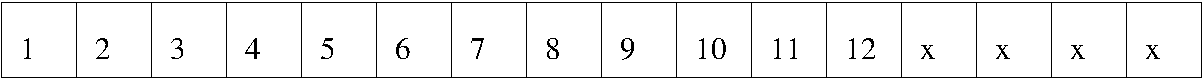
\includegraphics[width=120mm]{./images/1d_layout.pdf}
\end{center}
\caption{One dimensional layout of matrix}
\label{fig:1d_layout}
\end{figure}


\begin{figure}
\begin{center}
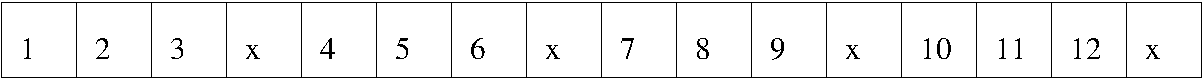
\includegraphics[width=120mm]{./images/2d_layout_row_mayor.pdf}
\end{center}
\caption{Two dimensional layout of matrix in Row Major format}
\label{fig:2d_layout_row_mayor}
\end{figure}

\begin{figure}
\begin{center}
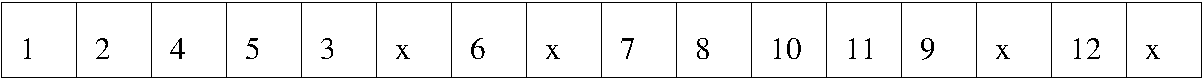
\includegraphics[width=120mm]{./images/2d_layout_fhb.pdf}
\end{center}
\caption{Two dimensional layout of matrix in FHB, Row-Major format}
\label{fig:2d_layout_fhb}
\end{figure}

Each number in the matrix takes up 4 bytes and a 16 byte alignment of
data is needed. Padding is written as \emph{x}'s.

%\begin{figure}
%\begin{center}
%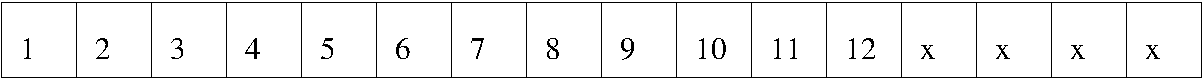
\includegraphics[width=120mm]{./images/1d_layout.pdf}
%\end{center}
%\caption{1d layout of matrix}
%\label{fig:1d_layout}
%\end{figure}


%\begin{figure}
%\begin{center}
%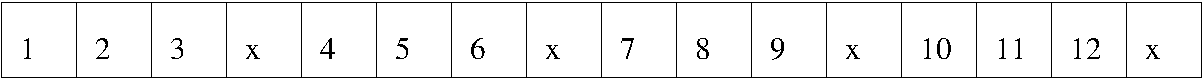
\includegraphics[width=120mm]{./images/2d_layout_row_mayor.pdf}
%\end{center}
%\caption{2d layout of matrix in Row Mayor format}
%\label{fig:2d_layout_row_mayor}
%\end{figure}

%\begin{figure}
%\begin{center}
%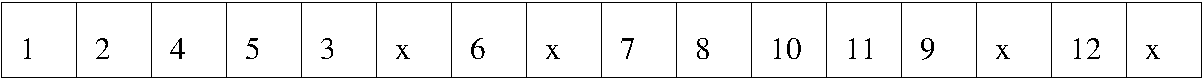
\includegraphics[width=120mm]{./images/2d_layout_fhb.pdf}
%\end{center}
%\caption{2d layout of matrix in FHB, Row-Mayor format}
%\label{fig:2d_layout_fhb}
%\end{figure}

In the layout shown in fig \ref{fig:2d_layout_fhb} a block size of 16
bytes is used for the \FHB\ layout.

When considering how an SPE would operate with these three memory layouts, let's look at each layout in turn, and describe some relevant features.

The order in which each layout is mentioned is intentional. For each new layout mentioned, it is implied that it can also be used as effectively
as the previous mentioned layouts.

\paragraph{One Dimensional Layout}
A one dimensional layout will effectively support all operations that are done element-wise.

\paragraph{Two Dimensional Layout With Row-Major}
This layout will make it possible to easily transfer separate rows to SPE's, since each row is stored aligned in the memory.
However, if a row is larger than what is accepted by a single SPE, additional computations are needed to remedy the situation.
(This can also be said for column major and in either case we might have a situation where neither a single row or a single column
fits into available space in an SPE's \texttt{LS}.)

\paragraph{Two Dimensional Layout With FHB}

The \FHB\ layout makes it possible to arrange data in a way, that
transfers are always easy to do, since each block is stored aligned in
memory and each part of a row in a single block is stored aligned in
memory. The dimensions of a single block can be chosen, so a data
block can always be made to fit in the \LS{}. Because of the structure
of the FHB format, it is also quite easy to index elements and find
which block a given element resides in. Of course, time must be spend
to convert data to the FHB format if the starting point is a
contiguous NumPy array, but when lots of computations are done on the
structure afterwards, the time spend on conversion is negligible. The
FHB format is preferred to the other two, since it allows for
non-element wise operations (like matrix multiplication), without the
need to waste processor time doing computations to locate data and
wasting memory bandwidth to transfer irrelevant data. As an example of
this problem, consider what would happen, if the one dimensional
layout were used to do matrix multiplication on the SPE's. In this
example we have to deal with the following issues:

\begin{itemize}
\item{Data alignment may not fit with the current row length.}
\item{It's somewhat harder to index elements in the array.}
\item{When doing matrix multiplications, each chunk of data on the individual SPE's may not
have an efficient structure.}
\end{itemize}

The FHB layout is described in \cite{scipy}, \cite{hp_storage_hybrid}
and \cite{blockhybridformat}. In these works, the structure is noted
for being effective for level 3 \BLAS\ routines such as matrix
multiplication, because of the blocked structure that gives better
data locality. An important aspect, is that the block size can be
chosen, so a block fits into the LS. The two
articles \cite{hp_storage_hybrid} and \cite{blockhybridformat} states
that the data locality obtained, using a blocked format, efficiently
makes use of the caching hierarchy on a regular machines. In the
context of this thesis and working with the Cell BE, the LS can be
compared to a large level 1 cache of a regular processor.

\section{The ndarray in NumPy}

The ndarray in NumPy is the single most important thing that NumPy
presents to the user. The ndarray is used to represent
multidimensional arrays and matrices. The rest of NumPy basicly
presents the user with ways of manipulating these arrays.

What is interesting, is to determine how the ndarray could be used on
the Cell BE and what modifications would be necessary to make on the
data layout and functions operating on the data layout.

It's assumed that \BLAS\ operations are extensively used in scientific applications, so they must be supported
efficiently for the ndarray on the Cell BE.

It must be decided if operations on ndarrays of more than two
dimensions should be carried out on the SPE's. Specifying element-wise
operations, the abstraction of extra dimensions is not important, but
if non-element wise operations are defined for ndarrays of more than
two dimensions, the data layout of each block in the FHB format
matters.


\subsection{Maximum Two Dimensional Array Operations on SPE's}

Several operations exist in NumPy that allows operations on arrays
larger than two dimensions. These include routines like addition,
multiplication and array-manipulation operations like view creation
and slicing. When doing operations on the SPE's, it becomes a big
issue how many dimensions there may be operated on. The general
assumption is, that NumPy is used for scientific computations. We find
it reasonable to assume that the larger part of a programs execution
time is spend on computation heavy operations involving arrays of
maximum two dimensions. This assumption is based, partly on the fact
that the arithmetic operations defined in the \BLAS\ library definition
involves no function arguments of more than two dimensions
(matrices). It's also assumed that the operations defined in the \BLAS\
definition are used extensively in typical scientific
applications. Scientific applications will therefore benefit greatly
from the possibility of running operations on no larger than
two-dimensional NumPy arrays in parallel on the SPE's. Operations like
view creation and slicing can be supported on the PPE.

Because no more than two dimensions are needed on the SPE's, a basic
requirement is that the FHB format must be used to represent vectors
and matrices. Scalars can be represented as a special case of vectors.

\section{The Data Format Selected For NumPyCBE}

The FHB layout seems like the best general choice, since it allows for
efficient non-element wise operations and can handle alignment issues.

NumPy's \emph{PyArrayObject} structure can be modified to contain meta
data to support the FHB layout. This meta data should include
pointers to all data blocks and data sizes. Furthermore, it might
prove advantageous to have additional information regarding whether a
specific block resides on a specific SPE. In this way, a DMA transfer
could be saved, if the data were found to already be located in
relevant \LS{}'s.

See section \ref{sec:extending_numpy} on
page \pageref{sec:extending_numpy} for a description of how meta data
is stored in NumPy to support the FHB format.

Data blocks in the FHB format must be squares of equal sizes.
This supports operations like level 3 \BLAS\ multiplication well.
Padding is inserted when needed to make the blocks square. 

\subsection{Storing Vectors}
\label{sec:store_vectors}

When using the FHB format to store vectors on the SPE's, it is
advantageous to make a distinction from the way matrices are
stored. If a new vector is created it makes no sense to store parts of
it using only one row of an entire block, leaving the rest of the
block empty. So instead it's chosen to use all space in the blocks to
store vectors.

\subsection{Shortcomings}

A general problem with the FHB layout is that it takes time convert
data to the format. In general, data conversions should be avoided as
much as possible.

Even though it's assumed that maximum two dimensional arrays are used
on the SPE's, there is an issue regarding performance if a matrix is
sliced from an ndarray of higher dimension. As an example, if a three
dimensional array is being sliced into a number of two dimensional
arrays and this slice is done on the "wrong" axis, a considerable
amount of clock cycles might be wasted by the PPE in order to
rearrange data. Figure \ref{fig:fhbslice} represents a bad and a good
slice. The first slice, A, makes a matrix across the third dimension, which
is clearly bad, since data must be rearranged to represent the slice in the FHB format.
The second slice, B, makes a slice, where the data
is already layed out correctly in memory.

\figscale{figures/fhb_two.pdf}{An example of a bad and good slice.}{fig:fhbslice}{0.6}


%\section{Additional rationale behind choosing FHB- REWRITE!!! and maybe move to conclusions?}

%When work began on this report, it was largely motivated by the master
%thesis \cite{scipy}. In this thesis an important conclusion
%is reached about the performance of IBM's BLAS routines optimized for
%the Cell BE. It is mentioned that IBM BLAS does not outperform an
%ATLAS implementation, even when the ATLAS routines only run on the
%PPE. We took this as a sign, that the data structure we should choose
%for porting NumPy's ndarray to Cell BE, must in itself support the
%splitting of data into easy manageable sub problems (e.g. a matrix A
%must be stored in memory, so that data can be split among SPE's
%without having to rearrange data first). Also, since IBM BLAS
%apparently did not perform well, we early on decided that we would
%have to implement our own BLAS routines, that would then perform very
%well with the FHB data layout, at least compared to the ATLAS and IBM
%BLAS results from\cite{scipy}.

%As work progressed, we learned that the results stated
%in \cite{scipy}, while being true, are not very useful. It seems that
%the test results from IBM BLAS were done without regard to the fact
%the IBM BLAS needs to run a single time first, to set up on the
%SPE's. After this single initiation, IBM BLAS has proved to be VERY
%effective. In\cite{scipy}, it is stated that IBM BLAS
%performs poorly because of this initial setup-cost. However, it seems
%that it makes no sense to make a test of IBM BLAS, were only initial
%setup-times are recorded. With the results we have seen in working
%with IBM BLAS, it performs very efficiently. So, while nothing wrong
%is stated in \cite{scipy}, it seems to us, that the results are very
%unuseful, and should not have formed the basis of our initial analysis
%for this master thesis.

%Ref til note om startup overhead: side 13 i http://www-01.ibm.com/chips/techlib/techlib.nsf/techdocs/F6DF42E93A55E57400257353006480B2/$file/BLAS_Prog_Guide_API_v3.0.0.3.pdf.

%BLAS1 and BLAS2 routines have shown to be more effective with IBM BLAS than using our FHB structure with our own BLAS implementation,
%and it is not likely that our implementation of BLAS 3 will be much better than IBM BLAS.

%We assume that IBM BLAS level 3 will use more time rearranging data, where the FHB layout makes data available without having to
%rearrange it, but the speed of the IBM BLAS routines themselves will likely be hard to beat.

%Because of this, we might have followed a different path in the report, if we had had more relevant test results. Instead of deciding early on to use FHB and
%custom made BLAS routines, we might have selected another option, like aligning and padding data in the existing ndarray and
%using IBM BLAS routines to operate on it.

%If IBM BLAS are used with non-contiguous data, an overhead must
%expected, under the assumption that the IBM BLAS implementation uses
%DMA lists instead of being able to transfer large contiguous data
%segments\cite{ibmblas_cell}. However, since BLAS 3 is computation
%heavy, this does not seem to be a big problem.

%In fact, it seems very likely that the NumPy ndarray layout should just be allocated on 128 byte boundaries and then be padded per row in
%order to be able to use IBM BLAS 3 routines effectively.
%(hele rationalet bag FHB var netop at IBM BLAS suttede til 1d layout. Dette skyldes sikkert Rasmus' resultater, som dog ikke direkte er beskrevet som
%vaernede udfoert med 1d data layout.)

%One test in \cite{scipy} page 56, shows that the FHB data layout beats IBM BLAS with a factor 32, but when the test setup that was used is taken into
%account, this test and its results are completely useless.

%\section{Multiplication with FHB}
%//illustrate how multiplication is accomplished with FHB.

%17/04/09 - This section is first attempt at a rewrite
%\section{Datastrucures for Numpy}
%With the assumption that NumPy is being used in a large variety of problem areas, the datalayout
%that is used for NumPy's NDArray must be selected carefully to generally support these areas well.
%It might be worth considering to convert betweeen different datalayouts during execution of a program,
%if this would speed up parts of the program execution time and the time to convert the data is deemed
%neglible in this context.

%Many operations used in scientific computing are done element-wise, where pairs of elements with equal indexes
%needs to be processed together, but no other dependencies exist between elements. For these kinds of operations,
%there is no obvious way to improve runningtimes by exploiting data locality (cache-tuning), so no specific demands
%can be deduced regarding an effective datalayout. In other words, it appears that many different datalayout would work
%equally well for these kinds of operations. The most important aspect seems to be, that time must not be waisted transferring
%elements to LS, if these elements not to be included in the operation at all. This places only minor demands on the datalayout.
%An example of af a datalayout that would not be very sufficient is one where lots of padding elements are included, since
%operating on these padding elements makes no sense.
%However, padding is essential for other operations to perform well.

%Other operations have a different kind of data dependency. The most obviou example of these are the
%matrix multiplication. In this operation a single element in the result matrix depends on elements
%from an entire row and collumn, respectively, from the two matrices. This means that care must taken
%selecting a datalyout that allows the data that shares the most dependencies to coexist in the LS.

%Other considerations must also be taken into account. The hardware specifications of the CELL BE puts
%some demands on the datalayout, if computations on it should be effective.

%As mentioned in [ref. to CELL afsnit], the following demands must be taken into account when analysing datalayout:

%\begin{enumerate}
%\item{Data alignment - in general, data must be 16 byte aligned for practical purposes
%(it is possible to transfer on alignments smaller than 16 bytes, but additional demands must be met in these cases).}
%\item{Data padding - padding is a means to ensure that alignment is maintained effectively.}
%\item{DMA transfers - a smaller number of large transfers are more effective than a larger number of small transfers.}
%\item{Cache lines - Cache lines are 128 bytes.}
%\end{enumerate}

%The datalayout for the NDArray should be useful in general cases. This means that no particular assumptions should be made about the input
%data. For instance, the data cannot be assumed to be aligned and in particular, it cannot be assumed that columns or rows in a
%matrix are aligned.


%A datalayout that seems interesting is the full hybrid block layout (from now on referred to as FHB).

%\subsection{FHB}

%Consider the following matrix:
%\[ \left( \begin{array}{cccc}
%1 & 2 & 3 \\
%4 & 5 & 6 \\
%7 & 8 & 9 \\
%10 & 11 & 12 \end{array} \right)\]
%To illustrate the FHB format the following three figures illustrate how this matrix could be layed out in memory.
%Figure \ref{fig:1d_layout} shows a one dimensional layout, with no padding. This layout would be sufficient for
%element-wise operations. Figure \ref{fig:2d_layout_row_mayor} illustrated a layout with padding. This layout makes
%it possible for rows or columns in a matrix to be aligned and thus enabling efficient transfers. An issue that
%must be taken into account with this layout is what to do, if a row of collumn cannot fit into the LS.
%Figure \ref{fig:2d_layout_fhb} illustrates the FHB layout. This layout can be used to split up a matrix into
%blocks that fit into the LS in a way that supports matrix multiplication.

%\subsubsection{Multiplication with FHB}

%\subsection{5-stencil with FHB}
%FHB is also useful for FHB - it might not be the best choice (Toennesen), but
%can still perform really good.

%\subsubsection{Some benchmarks using FHB from background material}
%backing up that FHB is good

%\subsubsection{Reality check - what performance can be expected from FHB with equally optimized versions using FHB and regualar 2d?}
%How should FHB be used and what could be expected?
%What could be expected when taking into account that some of Rasmus's results don't make sense.
%What is needed to use FHB as a general layout - i.e. support from venders etc.
%  - I denne forbindelse sammenskriv med opfordring fra side 207 i Anderson artikel.

%\subsubsection{Conclusion - is FHB a good choice?}
%What can be expected when using FHB and how thouls this thesis be structured because of that?

%\section{Other alternatives}
%A discussion of stuctures and what is best suited. Basicly a shorter recap of previous section.
%If a single structutre should be selected, FHB seems nice, because... even though...
%In practice there are problem: Using a custom layout... missing support...
%Other structures that makes more sense than FHB when taking vendor libraries into consideration? Can 2d layout be used easeliy with vendor libraries... Should this be
%suggested for practical settings? However - we use FHB as the general structure, but keep the points of practical usefullness in mind.. vendors must support FHB...



\chapter{SPU Programming}
\prepchapter
\label{chapter:dispatcher}
When building a complex program, such as NumPy, the program code can
usually not reside in the \LS\ of a \SPE{} in it's entirety. A key
observation is that, though the complete program is made up of several
functions, and presumably thus several megabytes of code, the
computational-intensive parts of each function only constitutes a
fraction of the complete program. These fractions can be split up
into \SPE\ programs that fit into the \SPE{}'s \LS{}.

In this chapter we will discuss and analyze the possibilities of how
to split up code, so it can be operational on
the \SPE{}'s.

\section{Uploading Programs to an SPE}

The naive and trivial way of uploading multiple \SPE\ programs, is to
develop them as separate \SPE\ programs and embed them into the \PPE\
program. In this way a new thread, for each \SPE{}, must be
created on the \PPE\ each time a new functionality is required. The \PPE\ thread
calling \function{spe\_context\_run()} is blocked until the \SPE\
program is terminated, either by failing or returning successfully.

This solution requires a lot of time creating and terminating
threads. Also, a full \SPE\ program must be transferred to each of
the \SPE{}'s \LS{}. This is not optimal. \\

A better solution is to have a static \SPE\ kernel on
all \SPE{}'s. This kernel should be the only \SPE\ program loaded by
the \PPE{}. Through this kernel, \SPE\ programs can be uploaded and
run on each \SPE\ without the need for extra thread creation.

First we will discuss the requirements for the \SPE\ programs and
lastly, we analyze the \SPE\ \ELF\ format to find a way to circumvent
the trivial way of executing \SPE\ programs. This will result in a final
specification for the \SPE\ programs and the basic means to do it.

Furthermore, on the way, we will gather information for requirements
for the kernel. How it should be developed and what features it should
have.

\subsection{Requirements for the SPE Program}

The system running behind NumPy, should be able to run the \SPE\
programs as fast as possible. This means, that transfering the program
to the \SPE{}'s, should be fast.

It might also be relevant to have a high level of control with the way
an \SPE{}'s \LS{} is partitioned. If the data layout of an \LS{} can be controlled,
it gives some flexibility regarding where to put program code and data.

Ideally, the following items are the key goals for making the system
execute the \SPE\ programs as fast as possible.

\begin{itemize}
\item{Create as few threads as possible}
\item{Transfer as little as possible}
\item{Create position independent code}
\end{itemize}

To attain the first, we need to exclude the trivial way of
executing \SPE\ programs and develop a specific kernel to do this job.

The second goal can be attained by only transferring the actual
program code that is needed, and not waste time setting up an entire
SPE context. This entails viewing program code as regular data. The
kernel should be able to have at least two buffers for \SPE\ programs,
for the ability to double buffer programs. This would hide the
latencies of transfering the programs and therefore no actual transfer
is requested when the program is needed.



To be able to run \SPE\ programs and to be as flexible as possible,
the \SPE\ program must be position independent. This means that the
program can be run from anywhere in the \LS{}. This also allows the
possibility for double buffering programs.

In his masters thesis\cite{cellcsp}, Mads Alhof Kristiansen discusses
ways of utilizing the \CBE\ to implement a framework for running CSP
programs. One of the issues he is dealing with is the fact the he
needs to be able to execute user-defined code on a \SPE{}. He
concludes that it is difficult(practically impossible), to use
position independent code, because the provided libraries from IBM are
not position independent and thus impossible to link with them. Nor is
it possible to recompile the libraries, because there is no available
source code for them.

A key difference between CellCSP and NumPy on the \CBE\ is, that
CellCSP has its user program the \SPE{}'s, while NumPy has its users
program the \PPE\ and then transparently incorporating \SPE\
functionality.

This difference entails that we know in advance, which libraries
NumPyCBE requires. Though it is impossible to link the libraries
to \SPE\ programs, the libraries can be linked to the kernel and
through function pointers, they can be available to the \SPE\
programs. Though this seems like a tedious solution, it actually
isn't. Almost all functionality on the \SPE{}'s is done with
intrinsics, see section \ref{sec:intrinsics} on
page \pageref{sec:intrinsics}. As intrinsics essentially are inline
assembly language instruction, they do not reside in a
library. Actually, the only library needed, is for a random number
generator.

\subsection{The SPE ELF Format}

When compiling an \SPE\ program using \program{spu-gcc}, an object
file is created in the \ELF\ format.

The \SPE\ \ELF\ format is composed of three sections. A data, text and
toe section. The text section contains the executable instructions of
a program\cite{elf}. This part of the \ELF\ file can be extracted by
disassembling the object file using \program{spu-objdump}.

The result of disassembling an object file, is the machine code
instructions given in plain text. Both given as assembler instructions
and as the machine code given in hexadecimal values. These hexadecimal
values can be extracted and used as functionality on the \SPE\ through
the kernel.\\

This information will serve as a starting point for development
of \SPE\ programs and the kernel.

\section{SPU Shaders}

SPU shaders are essentially functions created as described in the
previous section. The name originates from shaders in graphics, where
graphics hardware is programmed to calculate rendering effects. The
shaders gives a flexible way of programming the graphics processing
unit, instead of the fixed function pipeline seen in older graphics
hardware. Commonly, code fragments injected into a processing unit, in
this context a \SPU{} and inspired by \cite{spushaders}, is called a
shader or an SPU shader.

Likewise, the SPU shaders are meant to be a way to program
the \SPU{}'s in an easy and flexible way. In the following sections we
will analyze and discuss the potential of the SPU shaders and how they
are created.

%An example of the set of function pointers can be seen in code
%listing \ref{lst:fpointers}.

%\examplecode{code/functionpointers.c}{Example set of function pointers}{lst:fpointers}

\subsection{Creating SPU Shaders}

Only a few steps is needed to create an SPU shader. First of all,
since the SPU shader should be a flexible way of creating \SPE\
functionality, the kernel would not know anything about any function
requirements, both in the sense of arguments and return type. It is
therefore wise to specify a few function prototypes, to be able to
unify a possibly large collection of SPU shaders.

The set of prototypes should have argument lists that support all the
SPU shaders. Ideally, only one prototype should be made, but since
NumPy features a wide variety of functions, it is not likely to be so.

To keep the kernel as slim as possible(discussed in a later section),
the result of a function should be transferred directly from the SPU
shader to the \PPE{}. 

The prototypes argument lists could use the same idea as Python
does. Instead of having one prototype for functions with one argument,
one prototype for functions with two arguments and so on, an array of
arguments could be used or a structure of arguments. This forces the
SPU shader to handle the argument list by itself. This is not a
problem, since it knows which arguments it must expect.

Likewise, no return value should be used. Rather than having a static
return value, one or multiple of the arguments could be used as
references to return values.

An example of the finished prototype can be seen in
listings \ref{lst:prototype}.\\

\examplecode{code/prototype.c}{An example of a prototype for SPU shaders}{lst:prototype}

When the prototypes are designed the next step is to develop the SPU
shader. The SPU shader is developed just like any other C program,
though function calls must be handled differently.

Function calls to other functions should be inlined, because the code
should be position independent. Normal function calls are not
prohibited, but requires the called functions to be defined at a given
fixed offset, based from the calling function. This is not impossible,
but handling normal function calls requires extra work and linkage
overhead and should not be necessary.

The SPU shaders functionalities should not constitute an entire
program, but rather a single function. This prevents the size of the
function to explode and minimizes the number of function calls. Thus
typical function calls can be omitted and inlining used instead. As
indicated earlier, the \SPU{}'s functionality is obtained through
intrinsics, which are inlined assembly code and are not function
calls. And, as stated in section \ref{sec:loopunrolling} on
page \pageref{sec:loopunrolling}, inlining functions can reduce
function call overhead and again, SPU shaders should be small
functions, so the code size will not explode. \\

As it was mentioned before, the text section of the compiled code is
extracted. The text section is divided into a part for each C function
in the source file. Each of these parts can be used as an SPU shader.


The developed object file is disassembled with \program{spu-objdump}
into readable machine code instructions. The text part of the
disassembly can be transformed into code fragments or SPU shaders by
using the hexadecimal values of the machine code. The SPU shader can
then be put into the \PPE\ code as an array of unsigned integers and
then uploaded as data to the \SPE{}'s.

In listing \ref{lst:recipy} a step by step overview of the SPU shader
generation is shown. The first step compiles the code, but does not
link it, to an object file. The second step disassembles the object
files machine code instructions and the third step parses the
disassembled instructions and creates two files: one file containing
an array of hexadecimal values and one containing a binary output. See
section \ref{sec:oparser} on page \pageref{sec:oparser} for a more
detailed description of the parser script.

As an example, code listing \ref{lst:simple_shader} show a very simple
SPU shader, printing the number $123$ to the screen. Notice that an
auxiliary function is used for printing. This function is obtained using
the \variable{funcs} pointer given as input to the shader and is
explained in the section \ref{sec:disp}. The listing
in \ref{lst:simple_shader_disassmbled} shows the disassembled output
from calling \program{spu-objdump}. It shows the assembler
instructions and their corresponding hexadecimal values.

\examplecode{code/recipy.c}{Step by step overview of SPU shader creation}{lst:recipy}

\examplecode{code/simple_shader_code.c}{A simple SPU shader printing the number $123$}{lst:simple_shader}

\examplecode{code/simple_shader.o.dump}{A simple SPU shader disassembled}{lst:simple_shader_disassmbled}

\subsection{Using SPE Shaders}

Once an SPU shader is created, it must be transferred to
the \SPE{}'s. The \PPE\ must either load the code fragment from a
file, which is costly, due to disk accesses, but more flexibility can
be achieved, or it can be inserted directly in the \PPU\ code as an
array. In either way, the \PPE\ must inform the \SPE{}'s kernel, where
the SPU shader is. Once the SPU shader is in the \SPE{}'s \LS{}, the
kernel can run it through a function pointer, given the prototype as
discussed earlier.

When the SPU shader is finished, it returns to the \SPE\ kernel, where
another SPU shader can be run. Given the fact, that the SPU shader is
position independent, the kernel could have transferred another SPU
shader while executing the first. It only requires allocated memory
for both.

\subsubsection{When To Use SPU Shaders}

SPU shaders gives great flexibility. Running an application such as
Python, which includes a wide variety of functionality, it is
practically impossible to specify an \SPE\ program, that can feature
them all. With SPU shaders, one can upload arbitrary functionality
without transfering too much and without a switch of context.

But, with a restricted set of prototypes and limited access to
external libraries, it should not be regarded as a general solution
when programming SPE's. However, for porting NumPy, it seems like an effective
way of executing code on the SPE's.

\subsection{SPU Shader Considerations}

\SPU\ shaders can achieve good performance, because they do not
 require to implement a full \SPE\ program, but rather a single
 functionality. They omit the reinitialization of the \SPE\ for each
 functionality and only one \SPE\ context, the kernel, should be run
 from the \PPE{}.

But, if the SPU shaders become to large, any inlined functionality can
become problematic. If many inlined function calls are used, register
spilling can occur. See section \ref{sec:loopunrolling} on
page \pageref{sec:loopunrolling} for clarification.

Any debugging of an SPU shader is difficult. They require a suitable
testing environment, since they can not be run as is. For testing,
outputting functions can be established through a set of function
pointers. For example, a function for outputting a vector of floating
points or, as seen in code listing \ref{lst:simple_shader}, a function
to print out integers.

In scientific computing, the problem size can easily exceed the size
of the \LS{}. To handle this, the data must be transferred using
double or multiple buffers, as discussed in
section \ref{sec:doublebuffering} on
page \pageref{sec:doublebuffering}. This makes sure the data latencies
are hid. For each SPU shader run, each result needs to be flushed to
the \PPE{}, because the result is typically of the same size as the
problem.

For smaller problem sizes where all data can reside in
the \SPE{}'s \LS{}, the data latencies can, of course, not be hid,
but if the result is needed by the next operation, it can be kept in
memory on the \SPE{}'s to omit \DMA\ calls.


A fairly typical scenario, would be to have an operation taking two
arguments and producing one result, where the the result would be used
in the following operation. One of the arguments from the first
operation, might also be used in the following operation. So, when the
data can reside in \LS{}, some transfers can be omitted.

These optimization can, of course, not be applied when data is larger
than \LS{}. Though, a small optimization can limit the data latencies
by reversing the order of data blocks. That is, the order of the data
in the first operation is $data[0 \dots n-1]$ and in the second, the
order is $data[n-1 \dots 0]$. This would insure, that the last data
block in the first operation is done first in the second, to save a
block transfer. See a graphical representation of the idea in
figure \ref{fig:blockordering}.

%//A PIC OF THIS???

\figscale{figures/block_ordering.pdf}{Ideological ordering of the blocks.}{fig:blockordering}{0.6}

Any SPU shader should be created with the following in mind:

\begin{itemize}
\item{Too much inlining causes large code and risks register spilling(this can be detected with Cell simulator or by obtaining high running times).}
\item{The larger the SPU shader, the harder the debugging. Another reason to keep the shader as simple as possible }
\item{Data from small problem sizes can be passed on to the next operation}
\end{itemize}

With the SPU shader requirements in hand, it is time to define the
requirements for the kernel.

\section{The Dispatcher}
\label{sec:disp}

When the SPU shaders are implemented, the \SPE{}'s must be able to
receive them. This is the kernels job. This kernel will in this thesis
be called a dispatcher.

The dispatchers job is to get the correct SPU shader and its
corresponding arguments. Essentially, the dispatcher should establish
space in the \LS\ for the SPU shader itself, local memory for the SPU
shader and data blocks. 

Then, by demand from the \PPE\ part of the NumPy program, the
dispatcher should transfer information about the given SPU
shader. That is, the location of SPU shader and the given arguments.

When the SPU shader is transferred, the dispatcher executes the SPU
shader and waits for it to finish and then it is able to dispatch
another operation. \\

This section will contain an analysis of the dispatcher, what tasks it
should be given, how it can handle these tasks and administer the \LS{} memory.

\subsection{Tasks of the Dispatcher}

The dispatcher is the link between the \PPE\ program and the developed
SPU shaders. Because the SPU shaders are small program fragments, they
do not know anything about the layout of the \LS\ on
the \SPE{}'s. That is why, the first task for the dispatcher is to
organize the memory of the \LS{}. Next it must be able to receive an
operation\footnote{An operation is a collection containing an SPU
shader and its corresponding data and arguments} and finally,
terminate correctly.

\subsubsection{Memory Layout on the SPE}

To achieve optimal performance, the memory in \LS\ must be organized
in a manner, which suits all the developed SPU shaders, because
allocation and freeing memory can be expensive tasks when done
extensively.

Three chunks of memory, besides the memory given to the dispatcher
itself, must be allocated.

\begin{itemize}
\item{Memory to the SPU shader itself}
\item{Local memory for the SPU shader}
\item{Memory for data blocks}
\end{itemize}

These three chunks must be partitioned accordingly to the demands of
all the SPU shaders, since the memory should not be reorganized in a
later stage. It is possible to have an SPU shader with a alternative
demand of memory allocation, thus it should feature some
reorganization logics to alter the layout itself. 


%This extra logic consumes extra space and therefore less space
%for the data and extra time to reorganize the memory layout and
%therefore a bigger time overhead. 

The SPU shader can interpret the assigned memory in which ever way it
wants. The memory can be used as one big chunk of available data, not
needing to obey the guidelines provided by the dispatcher. The
assigned memory for data blocks, can be used for other things, as well
as the memory for meta data, can be used for other needs.

Figure \ref{fig:dispatcher_mem} depicts the \LS\ memory.

%\figscale{figures/dispatcher_layout.pdf}{Memory layout on the dispatcher}{fig:dispatcher_mem}{0.5}
\figscale{figures/ls_default.pdf}{Memory layout on the dispatcher}{fig:dispatcher_mem}{0.5}

The actual sizes of the chunks, must be defined by experimenting with
different layouts. Though the chunk for the dispatcher is determined
when it is fully implemented, including the local variables used and
the actual code.

The size of the memory for the data block partition depends on how
much data the \SPE{}'s needs or at least, how much it can hold at one
time. All the functions that will be implemented in this thesis,
demands at most five objects. Three arrays and two scalars. This is
seen with matrix matrix multiplication done in level three \BLAS{}.
Essentially, no subdivision for arrays and scalars should be done,
because they, in NumPy, inherit from the same object. The only
difference is the size of memory needed for data. Operating with
single precision arithmetics, only four bytes are required for
scalars, whereas much more memory is needed for arrays, depending on
their dimensions.

Using $64 \times 64$ blocks, which is the most common used size for
blocks, blocks of double precision floating point operations will
consume 32KB of memory. Using single precision, one block consumes
16KB. Partitioning the memory with double precision in mind,
capability of double buffering and needing blocks of data from three
different python objects, the memory for the data blocks uses $3 \cdot
2 \cdot 32KB = 192KB$.

The kernel should provide a pointer to each of the six blocks, though
the chunk is a contiguous memory partition and thus the SPU shader can
in theory use it to whatever it needs. This should remove any
considerations regarding letting the SPU shader reorganize the layout,
as mentioned before.

The rest of the memory is left for SPU shader memory, which is used
for internal dynamic memory used by the SPU shaders.

\subsubsection{The Memory Layout on the SPU Shader}

To let the SPU shader know how the dispatcher resolves the partitioning
of the \LS{}, the dispatcher creates a structure of pointers. 

This structure points to the parts of the \LS{}, where the SPU shader
can use memory. That is, the starting address of its own local memory,
the six pointers for the six blocks of data.

With this information, the SPU shader can make use of the \LS\ without
interfering with any of the other dynamically created data.

\subsubsection{SPE Identification}

As mentioned before, it is wise to have a standard declaration of the
prototypes for the SPU shaders. As discussed earlier, the dispatcher
does not need to know anything about the arguments for the SPU
shader. Nevertheless, as the dispatcher is the basic structure around
the SPU shaders, it is given a unique id for easy identification. This
id should also passed on to the SPU shader. The id spans from zero to
the number of \SPE{}'s used, minus one.

The unique id serves as a means to an effective parallel orchestration
of the data and it diminishes the contact to the \PPE{} while
computing in parallel. The \PPE{}'s role should be as little as
possible, as it was stated in section \ref{sec:ppe} on
page \pageref{sec:ppe}.

\subsection{Shader Control}

As discussed earlier, the dispatcher should be as slim as
possible. This is because, the less memory the dispatcher uses, the
more memory is left for computations and data. Also, the less the
dispatcher manages, the more control the SPU shaders have. When the
dispatcher have less control, the SPU shader can run in a less rigid
context. If the dispatcher should include functionality for the SPU
shaders, it should include an extensive library, which in turn left
less room for SPU shaders and actual data.

Another important feature of letting the SPU shader have all the
logic, is the developer can determine the parallel strategy. It is not
given that it should use ``bag of tasks'' or any dynamic or static
orchestration.

\section{Final Specification of the Dispatcher and SPU Shader}
\label{sec:specs}

To conclude this chapter, we will sum up some of the more important
requirements and specifications discussed and analyzed of both the
dispatcher and the SPU shader.

The dispatcher should be as slim as possible, because the most
functionality should be in the SPU shader. The following lists the
functionality specifications of the dispatcher:

\begin{itemize}
\item{Receive unique identification from \PPE\ }
\item{Initialize memory layout in \LS\ }
\item{Provide basic functionality from external libraries}
\item{Receive and run an SPU shader}
\item{Terminate the \SPE\ process when needed}
\end{itemize}

The SPU shader should implement the functionality for an
operation. Both in the sense of computing the data, but also getting
and putting data from the \PPE{}. The following lists the
functionality specifications of the SPU shader.

\begin{itemize}
\item{Initiate \DMA\ transfers}
\item{Orchestrate the data problem for parallelization}
\item{Compute the operation}
\end{itemize}



\chapter{Porting Numpy}
\prepchapter
\label{chapter:numpy}
The NumPy module is the center of attention in this master thesis. The
module and some of its more important data structures was introduced
in chapter \ref{chapter:python}.

An important motivation behind this master thesis is to open up for
the possibility of giving users of NumPy the power and flexibility of
utilizing the \CBE\ processor as seamlessly as possible. The NumPy
module has functions that can be ported to the Cell BE, and by doing
so let end-users execute Python applications without having to modify
anything in their programs in order to harness the power of the CELL
BE.

The NumPy module is implemented with sequential behavior and does not
take advantage of any kind of parallel hardware, so getting some of
NumPy's core functionality to operate in parallel in the Cell BE will
be significant achievement.


As work on this project began, the initial idea was to hook up all
Cell BE functionality in NumPy in such a way, that NumPy could be
installed just as originally intended, but also utilizing the \CBEv{'s}
SPE's. This means that the end-user would simply install NumPy on a
\PS\ or other CELL platform and not having to worry at all,
about doing Cell BE specific configurations or modifying any existing
Python applications. This would make it a completely seamless task
for an end-user to benefit from the power of the Cell BE when
executing Python applications.


A lot of work has been put into analyzing NumPy and doing a kind of
reverse engineering on NumPy, to be able to add functionality in the
right places. This proved to be a very time consuming process, because
the level of complexity of replacing certain operations in NumPy were
quite high and also because of the basic fact that NumPy takes quite a
while to install. As work progressed, it was chosen to build a
separate Python module instead, NumPyCBE. In this way the three
benchmark applications were run in versions that uses this separate
module instead of the original NumPy. This is only a minor issue,
since the functionality for running the benchmarks on the Cell BE
could easily be moved to NumPy, when a little extra work is spend on
analyzing NumPy code.


This chapter describes the work done analyzing and reverse engineering
NumPy. While it is definitely doable to extend NumPy with Cell BE
functionality directly, there was not enough time allocated in this
project to get to at point where all three benchmarks could run though
the modified original NumPy module. It was chosen, that it would be
better to run all benchmarks through a separate Python module, instead
of running some functionality through NumPy and some
functionality through a separate module.


We will discuss aspects of modifying NumPy, give small practical examples of how the modifications could
actually be done with NumPy and give hints and suggestions for future projects, where it might be considered to
extend NumPy in this way. The version of NumPy used is 1.2.1. Names of files and content may vary from version to version.



\section{Modifying NumPy}
\label{sec:extending_numpy}
NumPy consists of tens of thousands of lines of code spread across
multiple files. This section focuses on ways to port NumPy to the Cell
BE by modifying these files.

When NumPy is installed, many files are involved in the compilation
process. Some of these files are particularly interesting, because
they can be used to add and/or modify NumPy functionality. They will
be referred to later in this chapter. Here is a list introducing
them together with a short description.

\begin{itemize}
 \item{\file{ndarrayobject.h} This holds the definition of the
 \struct{PyArrayObject}. The PyArrayObject represents the ndarray. To add more
 meta data to the ndarray, this is the place to do it. Another file
 also holds structure definitions and these two files should be kept
 in correspondence. The other file is \file{numpy.pxi}.}

 \item{\textit{multiarrayodule.c} The file has many essential methods. Among
 these are methods that set up python variables
 (e.g. \function{setup\_scalartypes(...)}) and methods for manipulating
 ndarrays.}

 \item{\textit{arrayobject.c} This file holds many methods that
performs operations on ndarrays. This includes operations like
multiplication. Unary and binary functions work though Python by way
of Python's \function{PyCall\_Function} method that are called from
the functions \linebreak[5] \function{GenericBinaryFunction(...)}
and \function{GenericUnaryFunction} among others. When
\linebreak[5] \function{PyCall\_Function} is called, the control is given to Python. With the
call to Python, a parameter "op" is specified. It is assumed that
Python will use function pointers that has been registered as part of
the NumPy installation, if the "op" value specifies this. The file
also has methods for indexing ndarrays. This is used when slicing
e.g. matrices like A[1,:].}

 \item{\textit{ccompiler.py} In this file there are settings how
 compilation is done during an installation of NumPy. In this file it
 is possible to include libraries for linking etc.}

 \item{\textit{arraytypes.inc.src} and \file{scalartypes.inc.src}
 These files are written with tags that are replaced with actual
 type-information before compilation. In this way functionality is
 included for many different types.}

 \item{\textit{linalg.py} This file holds linear algebra functionality. Among
 other, this includes LU factorization (in the method "solve", which
 can be called with the same name directly from Python).}

 \item{\textit{ufuncobject.c} This file contains many math functions that
 operate on ndarrays in element wise fashion.}

 \item{\textit{genapi.py} This file contains a script that registers methods so
 that they will be callable from other parts of NumPy.}

 \item{\textit{umathmodule.inc.src} This file implements functionality for
 NumPy's Universal Functions (UFUNCS). UFUNCS are functions that
 operate on ndarrays in an element-wise fashion. Like the files
\file{arraytypes.inc.src} and \file{scalartypes.inc.src}, this file is first
 manipulated with a pre-compilation step, where a script replaces
 keywords in the file for actual types and operations in order to
 generate a set of functions for each type and operation. Functions
 defined in this file are typically called from functions defined in
 the file \file{ufuncobject.c}.}
\end{itemize}

The \struct{PyArrayObject} introduced in section \ref{sec:python-numpy}
on page \pageref{sec:python-numpy} can be extended to support
additional meta data that effectively allow the ndarray to be
processed using the SPE's. In chapter \ref{chapter:analysis} the FHB
data structure is selected as the preferred structure to be used in
this thesis. In code listing \ref{lst:pyarrayobject-numpybe} the
new \struct{PyArrayObject} can be seen. This structure has some new
fields that makes it more suitable and effective for use with the FHB
data structure and the Cell BE. The new additions are all placed in
the last part of the structure. In the following, each new addition to
the structure is listed with a short description. A few of these new
additions will be further explained later in this chapter. Some
padding is included in the structure to make it fit on exact 16-byte
boundaries. This is done because DMA transfers must be done with sizes
that are multiples of 16.

\begin{itemize}
\item{\texttt{blockData} points to an array containing pointers to the data blocks used in the FHB structure. They are layed out in row major order, not padded.}
\item{\texttt{numberOfBlocks} indicates how many data blocks the ndarray is comprised of.}
\item{\texttt{numberOfBlocksXDim} indicates how many blocks there are on the x-axis in the FHB structure.}
\item{\texttt{numberOfBlocksYDim} indicates how many blocks there are on the y-axis in the FHB structure.}
\item{\texttt{blockSize} indicates how many data elements there are in a single row within a data block.}
\item{\texttt{size\_in\_bytes} indicates the size of an element in the ndarray.}
\item{\texttt{paddingx} indicates how much padding there is included at the end of the last rows of the last block on the x-axis.}
\item{\texttt{paddingy} indicates how many rows that only include padding in the lower part of the blocks in the lowest row of blocks.}
\item{\texttt{slice\_info} points to a structure that contains information indicating where data is located, if the ndarray represents a sliced object.}
\end{itemize}

\examplecode{code/pyarrayobject_numpybe.c}{NumPy PyArrayObject}{lst:pyarrayobject-numpybe}


\section{Alignment Issues}
Since DMA transfers must be done on at least 16 byte alignments (128
bytes alignment is preferred if there is enough memory available,
because of cache line size), the objects that are created by original
NumPy code, must be copied to an aligned memory location if they
should be transferred to the \SPE{}'s. This likely applies to many of
the \struct{PyObject}s that represents ndarrays. A generic solution
would be to replace the allocation routine used be Python with one
like \texttt{malloc\_align} that can be specified to allocate space on
16- or 128 byte boundaries.

Also, be aware that any pointers that reside in the PyArrayObject must point to memory with legal alignment,
if data in this location is needed on the SPE's.

\section{Integrating NumPy With the Dispatcher}

%There is references to the dispatcher and shaders - should this section be moved, or is it ok?

Keeping the original design, where the end user should be able to
install NumPy as normal and start using the Cell BE through NumPy
straight away, the dispatcher and shader functionality, that is
developed for this thesis should be bootstrapped in NumPy.

This can be achieved by adding code to the appropriate NumPy
files. This section describes how this can be done and some of the
important and interesting things that happens (under the hood) hidden
from the user, to make NumPy effectively run on the \CBE{}.

\subsection{Starting the Dispatcher}
The dispatcher should be started once and then be available for the
entire duration of the Python program being executed. To facilitate
this, the dispatcher could be started in the
method \linebreak[5] \texttt{setup\_scalartypes(...)}, which is placed in the
file \file{multiarraymodule.c}. The functions itself has nothing to
do with the dispatcher, but starting the dispatcher here, has the
advantage that

\begin{itemize}
\item{the dispatcher is only started once and}
\item{the dispatcher is started when NumPy is imported into a Python program.}
\end{itemize}

When the dispatcher is up and running it is ready to receive signals from the PPE.

\subsection{Starting Shaders}
A function called in a program using NumPyCBE must have the same semantics,
from the users point of view, as the function call would have if NumPy was used.
In NumPyCBE the function is implemented either by code running on the \PPE\, the \SPE{}'s
or a mix. When code must be run on the \SPE{}'s, a shader is uploaded to each \SPE\ and
started.

What is interesting in the context of this chapter is how NumPy can be
extended with this functionality. Many of the function calls, that one
could imagine a program
calling passes through methods in the file \file{arrayobject.c}.
An example of this is multiplication, where the
method \linebreak[5] \function{PyArray\_multiply} is hit.

A convenient way to start shaders based on methods hit in this file, would be to remove
the call to functions like \function{GenericBinaryFunction} and \function{GenericUnaryFunction} and
instead call a custom method. This custom method could have a case-statement that takes into
account the arguments and type of operation that is needed and then upload the appropriate
shader to the \SPE{}'s.

By removing calls to the generic functions in \file{arrayobject.c},
the normal flow is stopped. This is an effect of Python not being
called using the \function{PyCall\_Function}. In the standard flow,
Python is given control over how to execute the given operation - this
is assumably done in Python by calling functions that are registered
in a Python dictionary when NumPy was installed. By stopping the flow,
Python is not given control over how to perform an operation and we
can effectively insert our own functionality that solves the problem
at hand using shaders etc.

This is just an example of where shaders could be started by hooking up the functionality in
the NumPy files. More practical examples are described later in the chapter.

\section{Deallocation}

When the reference count on a \texttt{PyObject} has reached zero, it
can safely be deallocated. Since the reference counter is placed in
the structure expanded by the macro \texttt{PyArray\_HEAD}, every
object has a reference count. For ndarrays, the
function \texttt{array\_dealloc(PyArrayObject *self)} placed in the
file \file{arrayobject.c} handles deallocation.

If the \struct{PyArrayObject} structure holds new members that
requires deallocation it must be added to avoid memory spilling.

\section{Data Conversion to FHB Format}
%//Hvor indsaettes dette i NumPy, eller hvor kan det indsaettes.
%//Der er udviklet en algoritme der omdanner data til FHB og generer noedvendig medata data baseret paa struktur ref.
%//Ref til kildekode i bilag X.

In NumPy there are some basic operations that must be supported. These operations
forms the basis of being able to use NumPy arrays effectively in applications.

An algorithm must be implemented to transform the data part of standard NumPy arrays into the full hybrid block format.
In NumPy data can exist contiguously or non-contiguously and the formats are typically C-style (row major) of
Fortran-style (column major).
If a contiguous row major layout is assumed, an FHB transformation as described in chapter \ref{sec:fhbdescription}, could easily be done.

For this thesis, transformations between one dimensional contiguous layout and FHB for ndarrays has been implemented.
FHB is used to support arrays of up to 2 dimensions. Additional dimensions are split up into multiple two dimensional FHB ndarrays.

The conversion function developed can be inserted in NumPy in function \texttt{\_array\_fromobject(...)} in file \file{multiarraymodule.c}.
This function is called every time an array is created using NumPy, and all meta data is available to be able to transform the data
into a FHB format using the new meta data on the \texttt{PyArrayObject}.

If the call to the conversion algorithm (named \texttt{numpy2FHB(...)}) is inserted in the last part of the function \texttt{\_array\_fromobject(...)},
more precisely after the \texttt{finish} tag as shown in code listing \ref{lst:numpy2fhb-insert}, the conversion takes place
right after the initial creation of the ndarray with data a contiguous one dimensional layout.

More precisely, it means that if an array is created in NumPy, like \texttt{A = array([[1,2],[3,4]])}, the array is converted
to the FHB format before being assigned to the variable A.

\examplecode{code/numpy2fhb_insert.c}{Calling numpy2fhb}{lst:numpy2fhb-insert}

%//Indsaet evt. et laekker illustration eller henvis til smaa eksempler fra data struktur afsnittet.

%When no slicing and broadcasting are done, maybe it would make sense only to transform matrices when they are needed?
%Then they could be transformed after normal NumPy operations (broadcasting etc.) and transformed back again after return.

%//Write where it makes sense to insert the transformation (in 105mult return and not where it is now... And make check for already allocated...)


%//write about FHB from nd arrays and the complications this will give (example with 3d cube.)

%//operations such as slice and broadcast (newshape?)

%//Hvor goeres det? Ekspel koert fra NumPy.

\subsection{Conversion of Multidimensional Arrays}
%//hvorfor er dette smart og hvad er ulemperne (slice paa tvaers og hvis der kommer hoejereordens (mere end 2-d) operationer, hvad hvis man foerst
%//konverterer arrays, naar det er noedvendigt - dvs. lige inden de skal bruges paa SPE'erne?).
%//Generelt vil vi gerne undgaa at kopiere data i main memory - dvs. vi vil helst oprette objekter der refererer til ekstereinde data,
%//men dette er vel hverken fortaler for at operret hele ndarray til FHB fra start, eller at gore det ad hoc...

As mentioned, code was developed to transform an entire multidimensional ndarray
into a two dimensional FHB format.

Figure \ref{fig:calletree} shows a recursive call tree. This
illustrates how a multidimensional array is transformed into one or
more two dimensional ndarrays with FHB layout. For each dimension, the
ndarray is checked to see how many dimensions of lower order exists
and recursive calls are made until the second dimension is
reached. When the second dimension is reached, the routine that
actually transforms the data are called with the appropriate indexes
to the data that exists within the given matrix.

In the figure, the contiguous one dimensional data array is
illustrated in the bottom. The syntax used is actual NumPy syntax, so
this specific array, if declared in NumPy, would result in an ndarray
with dimensions as specified. The function \variable{index} are used
to indicate the offset into the array for each call in the recursive
call tree.

\figscalerotate{figures/calltree.pdf}{Call tree}{fig:calletree}{0.55}{90}

One of the problems that could arise because
of this, is the time it would take to rearrange data, if a slice was
made on an inconvenient axis. If the ndarray was not converted from the
initial NumPy layout from the beginning, the conversion could instead
be done on-the-fly only for the specific one dimensional and two dimensional array that was
needed (remember, that max two dimensional arrays are handled on the SPE's).

Also, the one-time cost of converting data to the FHB format initially
could be saved, if data was not created in e.g.. a contiguous
row-major layout as it happens in NumPy by executing e.g. $A =
array([[1,2],[3,4]])$, but instead in FHB from the
start. If work on extending NumPy as described in this chapter is
continued, it might be interesting to locate the exact places in the
NumPy code, where the data creation is initially done.

However, as long as functions are implemented to work with the FHB layout, so it will not be necessary to do more data conversions,
the initial conversion to FHB should not be a performance issue.


%\section{A small practical example: How Numpy can be changed to implement a FHB layout}
%[todo - this subsection basicly describes how a Numpy array can be given a FHB layout, when an array is created in Python.
%This includes details about which functions to modify in Numpy.]

\section{NumPy API}
NumPy uses a specific way of handling it's internal API. A script
parses the source code files and registers methods. Therefore it is
import that the syntax be followed, if NumPy is expanded with new
methods that should be callable from other parts of NumPy. The
convention is to have the return type on it's own line and then have
the function name and parameters on the following line. The file
\file{genapi.py} contains a script that handles this. If additional files
should be searched be the script, they can be added in the file.

\section{Broadcasting}
Broadcasting is a NumPy term that expresses a functionality, by which
an ndarray is expanded on one or more dimensions so it can be part of
an operation involving another ndarray of larger size. While this is
an important aspect of using NumPy in general, it is not something
that is considered in this thesis. It is a trivial functionality and
one that can easily be avoided by writing test programs that only
operate on ndarrays, where the sizes are correct from the beginning.

\section{Porting Slicing and Indexing Routines}
Some basic routines that needs to be ported to be able to work with ndarrays are slicing and indexing.
\subsection{Slicing}
\label{subsec:slicing}
In the original NumPy module, slicing could be done on a matrix,
thereby returning a sub matrix e.g. a single row. If A is a
two-dimensional array created by executing this Python code:
\begin{center}\texttt{A=array([[1,2,3,4],[5,6,7,8]])}\end{center}
the slice \texttt{A[1,:]} will return the second row of the matrix.

When porting NumPy to the Cell BE and using FHB as the general data
structure, slicing should be handled with care, to make sure it is
still effective.

Because the general data structure is changed, slicing will also have
to be modified. To make slicing effective with the ported NumPy, it's
important that data is only moved when absolutely necessary. In
general, of course, but in particular in DMA transfers between the
SPE's and main memory. If a specific slice is needed on an SPE, it
would make sense only to transfer the slice and nothing else.

In the following we consider row-slicing
with a single full row. This is motivated by the \SOR\ test program that
is used for benchmarking. Later in this section we cast some light on issues
involved in supporting other forms of slicing.

To make slicing effective, code on the SPE should know which row to
move to its LS. It makes no sense to move an entire block of the FHB
data to an SPE, if only a small fraction of this block is actually
needed. Also, the overhead of initiating DMA transfers and calculating offsets
are better moved to the SPE's, so it's done in parallel and not to unnecessarily
burden the PPE.

The following NumPy functions in the file \file{arrayobject.c}
are involved in slicing a matrix (two dimensional ndarray) like \texttt{A[0,:]}:

\begin{itemize}
\item{\texttt{array\_subscript\_simple(...)}}
\item{\texttt{parseindex(...)}}
\item{\texttt{parse\_subindex(...)}}
\item{\texttt{getindices(...)}}
\end{itemize}

The method \texttt{array\_subscript\_simple(...)} takes a \texttt{PyArrayObject} as
input and returns a \texttt{PyArrayObject} representing the sliced part of the
input object. In the process of evaluating the body of the function,
the other mentioned functions are invoked.

What we want is, to move the slicing operation to the SPE's, since we
don't want to move a lot of data around for no reason. In the context
of this thesis it means that the shaders executing on the SPE's must
know if only a certain slice of a matrix should be fetched.

This is in perfect accordance with the way NumPy handles the slicing,
with respect to not copying data unnecessarily.

Consider the function \texttt{array\_subscript\_simple(...)} seen in code listing \ref{lst:pyarray-subscript-simple}.
\examplecode{code/pyarray_subscript_simple.c}{array\_subscript\_simple}{lst:pyarray-subscript-simple}

This function is called, when slicing the matrix \texttt{A} is done in
NumPy by executing e.g.. the statement \texttt{A[1,:]} on the
array \texttt{A=array([[1,2,3,4],[5,6,7,8]]}.
The \texttt{parse\_index(...)} function calculates the dimensions,
strides and offset of the data that should be represented in the
slice. This data will come in handy when slicing a single row using
the FHB structure with the \texttt{SOR} test program.

The information calculated in \texttt{parse\_index(...)} is used to
create a new \struct{PyArrayObject}, \texttt{other}, that has meta
data about the slice. Note that data is not copied, so the new object
points into the same data area as the parent object. A pointer to the
parent object is stored in the new object and the reference count on
the parent object is incremented by one, to make sure the data area is
not deallocated while the slice information is still being used.

When working with the FHB data structure and the SOR test program,
that specifically slices a single row out of a matrix at a time. The
slicing information we need to create on the relevant data can be
simplified somewhat. Since we don't use the original data-pointer in
the \struct{PyArrayObject}, but instead the
new \field{blockData}(array of pointers), we need to calculate where
the data needed is located in the old data format and find out which
row this corresponds to.

Since we allocate our FHB data contiguously within each block, the
strides information tell us if the slice is row or a column. The
pointer offset tells us where the initial data in the slice begins,
with regards to NumPy's original one dimensional data
structure. Because we know the size of our data blocks and each data
blocks has the same size (padding takes care of this), we can
calculate which row (or column) is needed in the slice. We can now
set meta data on the
\struct{PyArrayObject}, that the shader can read. The shader can then check if
the given \struct{PyArrayObject} actually represents a slice and the
just fetch the relevant data to work on.

In the case of the SOR test program, the only information about the
slice we need to tell the SPE's what row to use. Then each SPE can
transfer this specific row into its \LS{}. Notice, that the row is split
across as many blocks as there are blocks in the x dimension of the
FHB format. We can store meta data about a slice in a separate
\struct{SliceObject}. See code listing \ref{lst:sliceObject}. In this
\struct{SliceObject} we can tell if we are slicing a row or a column and
how many consecutive rows or columns we need. We can extend the
\struct{PyArrayObject} with this information by adding a pointer to a
\struct{SliceObject}, %as seen in code listing \ref{lst:sliceObject-insert}.
When an SPE receives a \struct{PyArrayObject}, it can now check if the
\struct{SliceObject} pointer is null, and if it is not, it only needs to fetch
the data specified in the slice.

If multiple rows were specified in the slice, the procedure is
analogues to the one for a single row, but it is a more involved
process if slicing a column, since data is stored in FHB, row major,
format.

Defining a stride to be the offset of getting from one element to the
next in a particular dimension. For a single column, there would be a
stride between each element, as large as the length of the entire
row. This would mean that more DMA transfers would be needed, where
each transfers involves less data than for the row-example. Some
overhead could be introduced to compute the index of the relevant data
within each DMA transfer. Another way of handling a large number of
column slices on a single matrix, could be to transpose the matrix
beforehand, so each column could be transferred using as few transfers
as possible. However, in order to see if the entire matrix is
actually needed, we would need to know what the python application
actually did before executing it, and this is not a very generic
solution. Another important issue to consider, when storing a
transposed version of a matrix, is memory usage. If the user has
calculated how much memory is needed for his data and NumPy suddenly
uses additional memory for copies of matrices, we could end up
swapping data to disk and thereby loose a lot of performance.

If we consider a two dimensional data layout, there is a small overhead involved
for each SPE in calculating the data to fetch, because it can be
spread across multiple blocks, but this overhead is negligible when
taking into account the time spend doing actual computations on the
data and considering applications like BLAS 3 multiplication, where
the FHB format really shines.


%//
%- Describe how subscript_simple is modified to return the same PyArrayObject as input,
%but with added SliceObject filled out.
%- Describe in what way parse_index is modified (or not modified, but how it's result is used)
%- Describe in what way the normal loop is disconnected (however that makes sense in NumPy).
%  (basicly how the inputarray is returned instead of the sliced copy! This is what is done in current custom NumPy!)
%  (if it shows that no time is saved by only adding metadata, just only hit on fact the metadata is available
%   for the SPE's).
%- YEAH YEAH, it is home no problem. Just don't create the other object, since it's not needed anyway.
%- As a sidenote, get to grips with decref/cref for the presentations and also document it in the dealloc section.
%- Check if NumPy actually copies data to other.
%  Data is NOT copied. METADATA on dimensions and strides are. Is this needed? If not it can be skipped.
%  However, what consequence does it have that this data might not be set?
%  If everything runs though "our" NumPy on CELL, is it not only decref we should be worried about?
%  So, whether we do slice on SPE or PPE, we can set the SliceObject on the SAME object? Thats a proposal at least.
%  The cool thing here is that functions that we implement where the PyArrayObject is passed, we can check if it
%  actually represents a slice :-). To make it wholly work in general, we should expand the function that prints values.
%  That is "A" instead of "A=...", so this function also only displays the slice only.
%  So for technical purposes we instead of creating a new PyArrayObject that points to slicedata we only set metadata
%  on the same PyArrayObject. Any downside? Yes, A[1,:] will be interpreted as the slice from now on!!!!!
%  So we need to return a new object, but extended with the SliceObject that is easier to interpret for our purposes.
%  Note that the original data on the new object could be used on the SPE's as well.
%  Illustrate the row/slice based on info from both sliceObject and the original data.
%  Also, if A is not used by itself, but only after a slice is indicated, the same object could be reused and
%  metadata would not have to be copied. The copy, in generel, is to make it more compatible with
%  NumPy and any future extensions that might be done.

%  So no SliceObject can come in handy to more easily tell the SPE what data should be fetched.
%  For instance, if is a single row, then the row can be signified with a single digit and a status
%  can tell the SPE that we need a single row.
%  And this SliceObject can be inserted here...

%  The SliceObject is important because we actually don;t use the regular stride and offset pointer
%  info any more!!! We don't maintain it - if we did, we could use it... But that is not part of the design.
%  
%  Maybe describe this bottom-up?

%  After that (incl illustration of fetching a single row from FHB for both origial data and SLiceObject),
%  Do the indexing section. Also, tell how a more generel slicing can be done (from old data or SliceObject - maybe just
%  SliceObject, if we prove this is also more effective for at singe row regarding computations on the SPE's).

%  INCREF/DECREF. Used internally and can be used externally. Make sure to incref new values - eg. return values.
%//

\examplecode{code/sliceObject.c}{sliceObject}{lst:sliceObject}

%\examplecode{code/sliceObject_insert.c}{sliceObject-insert}{lst:sliceObject-insert}



\subsection{Indexing}
%indexing is also an issue with FHB and the SOR testprogram.
%Check where this can be hacked (same place as with slicing?).
%The function PyArray_GetPtr in multiarraymodule.c produced a ptr that
%seems to be used for indexing into an ndarray.
%Catch it here and see if this a robust way to change this function
%to facilitate FHB :-)
%Yes, this is the way to go!

When indexing an ndarray, it can be done by executing the following
code: A[1,0]. When using FHB in row major it necessary to handle the
indexing differently, so the correct element is returned. This can be
done by changing the functionality of the
function \function{PyArray\_GetPtr} which is placed in the
file \file{multiarraymodule.c}. This function computes the index into
a contiguous array that holds the data of the ndarray, so instead of
computing the index on the basis of e.g. a contiguous one dimensional
layout, it should be changed to return the index into a specific block
and offset into that block for a FHB data layout.

This standard function for indexing can be seen in code listing \ref{lst:getptr}.

\examplecode{code/pyarray_getptr.c}{Example of original indexing}{lst:getptr}

The version that works with the FHB format chosen for this thesis can
be seen in code listing \ref{lst:index}. This version works for
ndarrays of up to two dimensions, and it takes into account whether we
are indexing into a vector or a matrix. This is a necessary check,
since vectors are layed out contiguously in the entire block. See
section \ref{sec:store_vectors} on page \pageref{sec:store_vectors}
for a description of the vector and matrix layout used in this
project.

The interesting parts of the code are the parts calculating which block and offset within the block
the indexed element is located at.

\examplecode{code/index.c}{Example of fhb indexing}{lst:index}

\section{Porting Functions}
%//Evt. en lille intro inden ufuncs og dette afsnit der beskriver forskellen paa de to kaldformer i NumPy.
%//Maaske denne lille intro skal staa inden genericbinary functions foerst naevnes? Ellers indsaet bare forud/bagud refs.
NumPy works as a kind of wrapper that can be fitted to run with a wealth of external libraries.
When porting functions to run on the Cell BE, there are two distinct ways that NumPy handles function invocations.
One of them involves calling generic functions that pass control to Python and the other involves calling
Universal Functions that are implemented in NumPy itself.

It seems the reason for using the generic calls, is so that external libraries (like a library implementing BLAS routines) can
be used by registering function pointers in Python when installing NumPy with specifications of what external
libraries to use.

In the following two sections, it is shown how both kinds of these function invocations can be ported to the Cell BE.

\subsection{GenericBinary and Unary Functions}

Some of the element wise functions that operates on ndarrays are
implemented by calling a generic function in the
file \file{arrayobject.c}. This type of function takes one or two
operands as input and an index for the operation to perform.

The generic function then calls python using invocation the function call \texttt{Py\_CallFunc(...)} to
perform the actual operation. See an example of the function \texttt{GenericBinaryFunction(...)} in code listing \ref{lst:genericbinaryfunction}.

\examplecode{code/genericbinaryfunction.c}{genericbinaryfunction}{lst:genericbinaryfunction}

As an example we consider addition. If two ndarrays are added
together, the function \texttt{array\_add(...)} placed in the
file \file{arrayobject.c} is called. The file is shown in code
listing \ref{lst:array-add}. This function calls the generic function
with a designated operation id to perform the actual operation.

To replace the existing functionality for adding ndarrays with new
functionality, it is possible to remove the call to the generic
function and instead call custom methods that performs the operation
on the SPE's instead. Both operands are available with the new meta
data added for use on the Cell BE, so this kind of extension is quite
simple.

\examplecode{code/array_add.c}{array addition}{lst:array-add}

\subsection{Universal Functions}

The standard \function{less\_equal} operation in NumPy is one of
several UFUNCS as they are designated in the NumPy manual. This
section describes the \function{less\_equal} functionality, but
other \texttt{UFUNCS} in NumPy are implemented in a similar way and
can thus be modified to run on the Cell BE using a similar procedure
as the one described in this section.

An element wise less equal operation on a vector and a
scalar\footnote{Or an array and an array} is performed internally in
NumPy by calling the function \function{ufunc\_generic\_call(...)},
from the file \file{ufuncobject.c}, with information about which
operations to perform and pointers to arguments. Next in the call
graph is the function \function{PyUFunc\_GenericFunction(...)}.

In this function an important call is made to the function \function{construct\_loop(...)}.\\
\function{contruct\_loop(...)} calls the function \function{construct\_arrays(...)}
 and returns a loop object pointer, \variable{UFuncLoopObject*} (show
struct in illustration etc.). This loop object holds pointers to
arguments, which are pointers to arrays for argument one, argument two
and the result argument. Since the second argument is a scalar, it is
represented as a \struct{PyObject} with a standard header and a value,
while the first argument and the result object are constructed as
\struct{PyArrayObject}'s.

The loop object also has a function-pointer registered, that tells
NumPy which function to call to carry out the \function{less\_equal}
operation. The pointer points to a function, that at pre-compile time
exists in the file \file{umathmodule.c.src}. When installing NumPy
this file is first preprocessed with a substitution step, where
certain keywords are replaced with actual data types etc. and then the
different versions of each function is compiled.
For \function{less\_equal}, a version using floats is created from the
"template function" named \function{@TYPE@@kind@(...)}. This function
does the actual computation in a loop that looks as seen in code
listing \ref{lst:less-equal}.

This loop shows how UFUNCS are implemented in NumPy in general by
replacing types and operations in the meta file \file{umathmodule.c}.
The loop is reused with different operations like equal, not\_equal,
greater, etc. For the \function{less\_equal} operation, the keywords
"@typ@" and "@OP@" are replaced and the resulting function is seen in
code listing \ref{lst:less-equal-actual-values}.

\examplecode{code/lessequal_loop.c}{lessequal meta loop}{lst:less-equal}
\examplecode{code/lessequal_loop_actual_values.c}{lessequal loop with actual values}{lst:less-equal-actual-values}

The name and return type of the function containing the specific loop
used for \function{less\_equal} with single precision floats is also set by
exchanging tags in \file{umathmodule.c}. The template prototype can be
seen in code listing \ref{lst:lessequal-function-name} and the actual
prototype can be seen in code
listing \ref{lst:lessequal-function-name-actual-values}.

\examplecode{code/lessequal_function_name.c}{lessequal meta function name}{lst:lessequal-function-name}
\examplecode{code/lessequal_function_name_actual_values.c}{lessequal actual function name}{lst:lessequal-function-name-actual-values}

In the loop the three operands of the less\_equal operation are used. The operand pointers are stored in the \texttt{bufPtr} pointer
returned from \texttt{contructloop(...)} call.

The key to making the less\_equal operation work on the Cell BE architecture is to create meta data the describes the data from
each of the three operands as being placed in data blocks, as corresponding to the FHB layout, and give control to the SPE's by
calling the dispatcher (see a description of the dispatcher in section \ref{sec:disp} on page \pageref{sec:disp}).


An issue that remains open, is where to make changes to the
functions \function{construct\_loop(...)}
and \function{contruct\_loop(...)} in order to return pointers to the
new \variable{blockData} array of pointers instead of the old data
pointer in the PyArrayObject (see section \ref{sec:extending_numpy}).

%intp is1=steps[0],is2=steps[1],os=steps[2], n=dimensions[0];
%  //char *i1=args[0], *i2=args[1], *op=args[2];


%\chapter{FHB - conversion and integration with Numpy}
%\prepchapter
%\label{chapter:fhb}
%\input{sections/fhb}


\chapter{Implementation}
\prepchapter
\label{chapter:implementation}
In this chapter, we will walk through the implementation of the
dispatcher and the Python module NumPyCBE. We will give a
conceptual walk through of the shader system as well.

The NumPyCBE module was implemented to be able to run our benchmark applications
through Python, using the same functionality as if the applications
were run through a modification of the original NumPy.

\section{The Dispatcher}

In this section the implementation of the dispatcher is examined. The
dispatcher has two major steps, which will be examined
chronological. First the start up phase and then when acting as a
state machine.

\subsection{Start Up Phase}

The dispatcher is started with a single argument. This argument is a
pointer to an \EA{}, where the \PPE\ places the operation
structure. The operation structure, is a structure that identifies a
NumPy operation and will be discussed later.

As it was discussed in chapter \ref{chapter:dispatcher}, the first
task for the dispatcher is to organize the \LS{}. The following list
sums up the demands for the \LS{}.

\begin{itemize}
\item{Space for the dispatcher itself}
\item{Space for shaders}
\item{Space for local memory for the dispatcher}
\item{Space for data blocks}
\end{itemize}

The space for the dispatcher can first be resolved when it is
implemented, but it should not consume more than 16KB.

The space for the data blocks was determined to be 32KB for each, that
is, 192KB in total, for six data blocks. This ensures, that exactly
six $64 \times 64$ blocks of double precision floating points can
reside in the \LS{}.

This leaves 48KB for the shaders and the local memory. The space for
the shaders are resolved by developing them. Basically, taking the
shader that requires the most space and dictate the space limits for
shaders to be that size. Of course, multiplying that with the number
of shaders required.

Due to the very sequential nature of Python and NumPy, one operation
is first executed when the previous is done. Practically, it does not
give any extra performance to double buffer the SPU shaders. The size
of the shader is typically a fraction of the data for one
operation. Though the time transferring the shaders are limited, it is
often nice to organize the shaders prior to a function. For example,
the function \function{solve} requires a handful of shaders and
setting them up inside function loops, transferring them and executing
them over and over, can give very large code sizes. We have therefore
decided, for this usage of the dispatcher, to have four buffers for
shaders.

\subsubsection{One Dispatcher, Multiple Layout Schemes}

The diverse needs for the dispatcher has led to an implementation,
accompanying them all as good as possible. Given a set of definitions,
the dispatcher can be build with an almost arbitrary layout.

This master thesis focuses on single precision computations, therefore
the data block buffers does not need to be exceptionally large and
thus the remaining memory of the \LS{}, can be used elsewhere. If
double precision was used, the dispatcher could be build to accompany
those.

It is not necessary to have buffers for four shaders, so for another
use, the dispatcher could be build for only one. The size of the
shader buffer is sized by experimentation and the actual need. This
size is fixed at 12 KB.

Figure \ref{fig:lspartition} depicts the layout of the \LS{} using one
buffer for shaders and buffers large enough for $64 \times 64$ double
precision data blocks. Figure \ref{fig:lspartitionused} shows the
layout of the \LS\ used in this master thesis. Giving enough space for
$64 \times 64$ single precision data blocks, four shader buffers and
plenty of local shader memory for array meta data.

\figscale{figures/ls_v2.pdf}{Layout of the local storage for double precision}{fig:lspartition}{0.65}

\figscale{figures/ls_v2_fourshaders.pdf}{Layout of the local storage used in this thesis}{fig:lspartitionused}{0.65}

\subsection{The State Machine}

When the layout of the \LS\ is organized, the dispatcher waits for the
\PPE\ to signal an operation. This is done by mailing an integer from
the \PPE{}. Each number mailed from the \PPE\ determines a specific
state for the dispatcher and the dispatcher transfers the operation
structure from the \PPE{}.

The structure identifies the shader for the specific operation, its
size, the operands and how many \SPEv{'s} used. The structure can be
seen in figure \ref{fig:operationt}.

\figscale{figures/operation_t2.pdf}{The operation structure}{fig:operationt}{0.65}

As it can be seen, the three objects and the two scalars are
separated, though their meta data is the same. This separation is done
to be able to distinguish between objects containing more than one
data element, i. e. arrays, and a single scalar.

The main difference is location in the \LS{}. Any array object should
be put into the designated block areas. That is, the last six fields
in figure \ref{fig:lspartition} or \ref{fig:lspartitionused}.

The number of \SPE{}'s is also given as a field in the structure. This
gives a specific \SPE\ information about how to orchestrate the data
for parallel computations. It is therefore not necessary to utilize all
the \SPE{}'s for one operation. Especially, if the number of blocks
for a given operand is less than the total number of \SPE{}'s. Though,
as argued before, Python is executing operations sequentially and
therefore any superfluous \SPE{}'s can not easily be utilized
elsewhere.

The \EA\ of the shader, in the operation structure, lets the
dispatcher transfer the actual shader to the \LS{}. When transferred,
it is run with one of two function pointers.

By examining the functionality of NumPy, two prototypes for function
pointers to shaders are needed. These two prototypes can be seen in
listings \ref{lst:prototypes}.

\examplecode{code/prototypes.c}{The two prototypes for SPU shaders used in this thesis}{lst:prototypes}

As it can be seen, one thing differs. The \variable{EA\_result} in
\function{runr()}. This prototype is used when a NumPy function
returns a single scalar value, rather than an entire array.

The need for this division is, when multiple \SPE{}'s computes their
own part of the result. In the \function{sum} shader, each \SPE\ sums
their parts, but each of the \SPE{}'s intermediate results should be
combined, not stored in the same scalar value given by the operation
structure. For these types of operations, the \PPE\ establishes space
in main memory for each of the \SPE{}'s results, and then the
\PPE\ combines the result. When a shader needs to return an array, a
pointer to this array is given as a field in the operation structure.

The \variable{EA\_result} address is mailed to the dispatcher from
the \PPE{}, before the dispatcher runs the shader, thus letting the
shader know where to put the result after calculations.

The state machine can be examined in figure \ref{fig:statemachine}. It
shows how to make the dispatcher behave and interpret the given
operation. States 0 and 100 is the most commonly used, they receives
an operation and executes it. State 200 and 400 receives an operation
and a shader, with no return value and with return value,
respectively, without executing it and state 300 and 500 executes the
shader. These two last states makes it easier to implement composite
functionality. It is possible to transfer multiple shaders without
running them and running shaders, already in the \LS{}, without having
to transfer them first. Lastly, state 999 terminates the dispatcher
process.

\figscalerotate{figures/statemachine_v4.pdf}{The SPE state machine}{fig:statemachine}{0.55}{90}

\subsection{Putting It All Together}

A diagram of the complete process can be seen in figure
\ref{fig:speppe}.

The relation between the \PPE\ and the \SPE\ is given by the initial
argument, which is a pointer to a certain part of the main
memory. When an \SPE\ receives a new state from the \PPE{}, through
mailboxes, it knows where to get the operation, because the argument
points to an address space, where a pointer to the operation is. From
the operation, the \SPE\ can get further information of the operands
and the given shader for this operation. The address of the
\variable{SPE pointer address} is given to the \SPE\ as an
argument. The value of \variable{SPE pointer address} is set by the
\PPE\ to point to an operation, from where the dispatcher can obtain
the address of the operation.

When an operation is in progress, the SPU shader transfers the
operands and transmits the final result.

\figscale{figures/speppe.pdf}{The PPE SPE relation}{fig:speppe}{0.45}

\section{SPU Shaders}

As stated in section \refthis{sec:specs}, the SPU shader has full
control over data transmissions. This implies, that the SPU shader
control double, or multi buffering, of data. Instead of letting the
dispatcher handle this, the individual SPU shader can decide which
method that fits best in a given situation.

This is also true for the orchestration of the data. This may be
static or dynamic, bag of tasks or streaming. Which ever method that
works best in the given situation, problem size or with the
computational requirements.


\subsection{Generic Functionality}
\label{sec:genericfuncs}

Much of the ndarray core functionality provided by NumPy are binary
or unary functions. All of which are element wise
computations. Typically, they are composed of one of the following:

\begin{itemize}
\item{Array - Array}
\item{Array - Scalar}
\item{Scalar - Array}
\end{itemize}

For example, array multiplication can either multiply two arrays
together, element wise, or multiply a scalar to each of the elements
in the array. That is, scaling the array by a constant factor.

In these functionalities, each \SPE\ acquires a certain number of data
blocks, given the number of total \SPE{}'s used and its given
index. Moreover, almost all of the functionalities returns their
results in an array. Given these identical specifications, a common
framework can be implemented to generalize these kinds of operations.


In code listing \ref{lst:genericshader}, in appendix
\refthisnotitle{app:gbff}, the framework for the generic binary shader
function for two arrays is shown. As it can be seen the function has a
preliminary unresolved inclusion, which, by a parser, is resolved
prior to compilation.

Also, the actual function call \function{\_compute}, has its arguments
resolved with the same parser. This parser is discussed later.



An example of the \function{\_compute} function can be seen in code
listing \ref{lst:genericadd}, in appendix
\refthisnotitle{app:g-addition}, where the element wise addition for
two arrays is shown.



This is done by a Python script, parsing a template C file. For each
of the functionalities, a header file defines the same function name,
but implements different functionality according to the NumPy
function. The header file inclusion is replaced by Python in the main
template code.

\function{Multiply}, \function{add}, \function{divide} and
\function{less\_equal} are examples of functions that can take both
arrays and scalars as arguments and returns an array as a
result. \function{Sum} is an example of a function that takes a single
array as argument and produces a single scalar as result. 

Filler functions are also examples of functions that can be
generalized. For example \function{zeros} and \function{random}, they
only take one array as argument and returns the same array filled with
the values needed. 

\subsection{The Object File Parser}
\label{sec:oparser}

The object file parser is a tool, written in Python, to parse the
object file given by compiling a C source file. It extracts the
numerical values of the dumped object file, given by
\function{spu-objdump} to form a header file, ready to be included
directly in a \CBE\ program and a binary file, that can be loaded at
run time, by a \CBE\ program. This sequence of values can be
transferred to the dispatcher as shader.

\section{NumPyCBE}

As a consequence of how long time it took to analyze and work with
NumPy, we decided, as stated in section \ref{chapter:numpy}, to
develop our own Python module with the same functionality as
NumPy. This section will give a quick overview of the implementation
of this module.

The module must allow Python applications to utilize the Cell BE. To
meet this goal, the dispatcher and shader system was used in the same
way as if it was used with a ported version of NumPy.

The module should be able to execute a Python program like the one
shown in code listing \ref{lst:mc}. Note that if infix operators were
used in this program, it would have the same syntax as one written for
the original NumPy.

\examplecode{code/mc.py}{Monte Carlo example}{lst:mc}

Since all the functionality for working with ndarrays is implemented
in C files in the NumPyCBE module, there is no need for representing
Python objects of entire ndarrays in Python. It is only necessary to
store pointers to ndarrays and actual scalars in Python. In this way
regular scalar-scalar operations can be handled directly in Python,
while the rest is handled by C code in NumPyCBE. Therefore, the only
values that are passed between Python and the module are scalars and
pointers to ndarrays.

Each function should be callable from Python must be defined in the
module.  This is done by creating a structure like the one shown in
code listing \ref{lst:pymethoddef}. In this example only one function,
\function{add}, is defined and the number of arguments to the
functions are set to be variable.

The structure
of function definitions is passed to the \function{initnumpycbe(...)} function in the module, which can be seen in code listing \ref{lst:initnumpycbe}.
This function is by convention the first function called by Python when a module named NumPyCBE is imported.

\examplecode{code/pymethoddef.py}{Python method definitions}{lst:pymethoddef}
\examplecode{code/initnumpycbe.py}{Initialization function for the NumPyCBE module}{lst:initnumpycbe}

When the \function{initnumpycbe(...)} function is called, the module is registered by name in Python.
Notice that a call to start up the dispatcher is included in the function.
In this way the dispatcher is started on each SPE when the \function{numpycbe} module is imported into a Python application.

When a function in the module is called from Python, zero, one or more
\variable{PyObject}'s are given as parameters.  These must be parsed
in the receiving function and a \variable{PyObject} must be returned
as the result of calling the function.  As mentioned, we only need
pointers and scalars in NumPyCBE. An example of how the parsing and
handling of input parameters and return value are done, can be seen in
code listing \ref{lst:add}. In this example the variables \variable{a}
and \variable{b} are used to hold pointers to
\variable{PyArrayObject}'s. The actual addition is done in the
function \function{run30(...)}(which is discussed in section
\refthis{sec:runshaders}). Notice that the return value in this case
is the address of the first operand, wrapped in a \variable{PyObject}.

\examplecode{code/add.c}{add function}{lst:add}

When all necessary functions are defined and implemented in the c-file \file{numpycbe.c},
the module can be installed be executing the following statement: \texttt{``install setup.py install --prefix=.''}.
This uses the file \texttt{setup.py}, shown in code listing \ref{lst:setup} to install the NumPyCBE module.
Note that the \texttt{libspe2} library is added for linking in the setup file, since this functionality is needed
to work with the SPE's on the Cell BE.

\examplecode{code/setup.py}{setup.py file for NumPyCBE}{lst:setup}

Notice that the \texttt{prefix} keyword is only used to install the module in a specific location.

After installation, the module can be imported as shown in the
beginning of the test program in listing \ref{lst:mc}.

\subsection{Running Shaders}
\label{sec:runshaders}

When NumPyCBE is running a shader, it requires the actual shader,
given in an array, and the size of the array in bytes. It must
differentiate between functions returning scalar values and
functions returning arrays, as discussed earlier in this chapter.

Furthermore, shaders require up to three arrays and two scalars as
arguments, for both versions. If two different shaders needs the same
number of arguments, they can be run identically. This can generalize
to a set of functions, running shaders with a different number of
arguments. As it was seen in listing \ref{lst:add}, three arrays were
needed and zero scalars. Thus calling the function
\function{run30()}. If a shader needs to arrays and one scalar, the
function \function{run21()}, should be called. 

The shaders returning scalars, have an almost identical counterpart,
named \function{runrxx()}, where the x's are substituted with the
number of arrays and the number of scalars in the argument list. The
``r'' identifies, that the function returns a scalar value.

\subsubsection{Dynamic SPE Handling}

The functionality, mentioned before, also handles the data
orchestration indirectly. This means, that it determines how many
\SPE{}'s are going to be used. Primarily based on how much data is
present in the given ndarrays. Some NumPy functions require even less
work, even though much data is present. Multiplying a sliced ndarray,
could be an example. When special circumstances are required, the
NumPyCBE function itself handles the \SPE\ contact.

%\subsection{FHB Tool}

%Several functions are needed to work with \FHBv{ing}, especially when
%creating an array using the layout. Therefore, a library was developed
%to ease the tasks when working with \FHB{}. 

%This library contains functionality creating arrays in different ways,
%both as vectors and matrices: Creating arrays with one default value
%for all elements, creating arrays within a specific range, with a
%%given step size, creating arrays with no default value, that is only
%initialize the memory, filling arrays with certain values, extracting
%columns from matrices and much more.

\subsection{Handling FHB}

To handle \FHB\ ndarrays on the \PPE{}, a library was created. This
library takes care of creating and destroying the ndarrays, as well as
convenience functionality, such as extracting a column from a matrix,
calculating block offset and indexes, and printing ndarrays.

\subsection{Allocation/deallocation}
Currently, NumPyCBE does not make use of Python's object deallocation mechanism.
Therefore allocation and deallocation of arrays and scalars must be done explicitly
in the Python application.

\section{Limitations}

In our implementation, we use the fact that only 256MB(actually an
average of 150MB) of RAM is available, thus giving us a problem size
of two matrices of maximum $4096 \times 4096$ single precision
elements. Therefore, a maximum of 4096 pointers needs to be used in
the field \variable{blockData} in the data structure. This requires
16KB of storage for each matrix used and is easily managed into the
\LS{}.

For arbitrarily large matrices, this fact can not be used, because the
size of the meta data would exceed the \LS{}. A solution to this,
could be to transfer parts of the \variable{blockData} array as
needed. This would not require much restructuring of the shaders, but
would require extra logic and possible extra data transfers of the
meta data.


\chapter{Test Programs}
\prepchapter
\label{chapter:testprograms}

For this master thesis we have selected three different tests:
\textit{Monte Carlo $\pi$}, \textit{linear equation
  solver}(solve) and \SOR{}. These three tests should explore the
  possibilities of the
\CBE\ as best as possible and give the opportunity for utilizing the
programming techniques described in \REFSEC{sec:considerations}.

%section \ref{sec:considerations} on page \pageref{sec:considerations}.

They will also show tests of NumPy parts using both simple and
composite functionality, from \REFSEC{sec:performanceoncell}.

The shaders developed for these tests are all using a static
orchestration of their problem. This particular segregation is primarily
because we know how many \SPEv{'s} are available, but also because
the test programs will operate on data for easy static orchestration.

Furthermore, the individual shaders utilizes at least double buffering
and \SIMD\ operations. Where possible, dual issue is used and excess
transfers are removed.


\section{Monte Carlo}

Monte Carlo is a method that relies on repeated random sampling. It is
a type of computational algorithm and can be used to estimate $\pi$.

Having a circle with radius $1$ inclosed in a square, the area of the
circle is $\pi$ and the area of the square would be $4$. The circle
fills up $\frac{\pi}{4}$ of the square, that is the ratio of the
circle to the square. The area of the circle can be calculated by
multiplying the ratio with the area of the square, that is
$\frac{\pi}{4} \cdot 4 = \pi$. 


%See figure \ref{fig:circle}.


%\figscale{figures/circle_in_square.pdf}{A unit circle inclosed in a unit square}{fig:circle}{0.4}
%// PIC OF THIS

The area of the circle can be approximated using Monte Carlo
$\pi$. Imagine shooting randomly at the square, the probability of
hitting the circle, is exactly $\frac{\pi}{4}$. So, shooting $n$ times
at the square, $\frac{\pi}{4} \cdot n$ of them will hit the circle. If
$i$ shots hit the the circle, the ratio would be $\frac{i}{n}$, which
is the circles area, $\pi$.

\subsection{Implementation}

The Monte Carlo $\pi$ test program was based on Brian Vinters
implementation. Only a slight adjustment was made to it, since NumPy
natively uses double precision. This should ensure that the precision
in the test programs were identical.




When implementing the Monte Carlo $\pi$ a set of points, (x, y), must
be generated. Because most random number generators produce numbers in
the range $[0, 1[$, the problem can be reduced to the positive
    quadrant of the unit square and circle. This implies, that
    the generated point (x, y) must satisfy $x^2 + y^2 \le 1$.

Given this, five shaders must be implemented:

\begin{itemize}
\item{Array Random Filling}
\item{Array Multiplication(or Array Square)}
\item{Array Addition}
\item{Array Less Equal}
\item{Array Summation}
\end{itemize}

The result from the summation can trivially be multiplied by $4$ and
divided by $n$ by Python, wherefore no further shader functionality is
needed.

%In section \refthis{sec:mc_code}, the Monte Carlo test program can be
%reviewed. Both the original and the slightly adjusted NumPyCBE
%version.

%\subsection{Cell Blade Center and Cell Clusters}
%
%This test should be applicable to a Cell Blade Center and even
%clusters of these. The key thing to notice is, that the data is
%generated on each \SPE{}, local to its own \PPE{}. While processing
%the operations, no data is needed to be transferred between the Cell
%processors, only when the final result is joined.


\section{Solving Systems of Linear Equations}

Solving systems of linear equations of the form,

\[
Ax = B
\]

\noindent with $n$ equations and $n$ unknowns and where $A$ is the coefficient matrix, $x$ is a vector of
unknowns and $B$ is the right hand side, it can be solved with
Gaussian elimination.

This requires $O(n^3)$ operations for each set of right hand sides. If
the same coefficient matrix should be used to solve several other
linear equations, LU factorizations should be used. An LU
factorization also takes $O(n^3)$ time and solving it only takes
$O(n^2)$, but the LU factorization is only computed once.

The \LAPACK\ routine \function{xGESV} does exactly this. It takes two
matrices as input, the coefficient matrix $A$ and the set of right
hand sides, matrix $B$. $B$ contains the columns of results for each
of the equations. At the end of the routine, each column of $B$ will
contain the values of the unknowns for each set of right hand sides.

First the theory behind the solver is examined and then it is
explained how it was implemented.

\subsubsection{Blocked LU Factorization Algorithm}

The \LAPACK\ routine \function{xGESV} solves the equation $Ax = B$,
with an LU factorization with partial pivoting and row interchanges,
of the form,

\[
Ax = B \quad \Rightarrow \quad PLUx = B
\]

\noindent where $P$ is a permutation matrix, $L$ is a lower triangular
matrix with a unit diagonal and $U$ is and upper triangular matrix
with a non-unit diagonal. $L$ and $U$ are of the form,

\[
\mathbf{L} = \left[
\begin{array}{ccccc}
1       & 0     & \cdots &   \cdots  & 0 \\
M_{21}  & 1      &        &          &\vdots \\
M_{31}  & M_{32} & \ddots &          &  \vdots \\
\vdots & \vdots & \ddots &  1       & 0 \\
M_{m1}  & M_{m2} & \cdots  & M_{mm-1} &  1 \\
\end{array}
\right]
\quad
\mathbf{U} = \left[
\begin{array}{ccccc}
M_{11}  & M_{12} & M_{13} &  \cdots  & M_{1m} \\
0       & M_{22} & M_{23}  & \cdots  & M_{2m} \\
\vdots  &        & \ddots &  \ddots &  \vdots \\
\vdots  &        &        &  M_{m-1m-1} & M_{m-1m} \\
0       & \cdots & \cdots  & 0      &  M_{mm} \\
\end{array}
\right]
\]

The first thing to do is to factorize $A$. This is done by the
\LAPACK\ routine \function{xSGETRF}. This function uses a blocked
algorithm to compute the LU factorization, for a block size of $r$ on
a matrix of size $M \times N$. The overall idea is illustrated in
figure \ref{fig:blockedlu}. It should be noted, that A(0,0), for
example, is a sub matrix.

%// Show an illustration of this
\figscale{figures/a-lxu.pdf}{Block LU factorization, where A is an $r \times r$ sub matrix, A(0,1) is $r \times N-r$, A(1,0) is $M-r \times r$ and A(1,1) is $M-r \times N-r$}{fig:blockedlu}{0.5}

The idea is to compute the block columns of $L$ and block rows of $U$
iteratively. From \cite{LU_blocked_algorithm} we have,

\begin{align}
L(0,0)U(0,0) &= A(0,0) \label{lu1} \\
L(1,0)U(0,0) &= A(1,0) \label{lu2} \\
L(0,0)U(0,1) &= A(0,1) \label{lu3} \\
L(1,0)U(0,1) + L(1,1)U(1,1) &= A(1,1) \label{lu4}
\end{align}

\noindent Where equation \ref{lu1} and equation \ref{lu2} performs the
LU factorization of the first column block, $A(0,0)$ and
$A(1,0)$. With these results $U(0,1)$ can be calculated.

Equation \ref{lu4} can be rearranged to 

\[
A'(1,1) = A(1,1) - L(1,0)U(0,1) = L(1,1)U(1,1)
\]

Finding $L(1,1)$ and $U(1,1)$ can iteratively be reduced to finding
the LU factorization of $A'(1,1)$ in $K$ steps, where $K = min(\lceil
M / r \rceil, \lceil N / r \rceil)$. After $k$ of $K$ steps, the first
$k \cdot r$ column of L and rows of U have been evaluated. The matrix
A have been updated as shown in figure \ref{fig:updatelu}. The sub
matrix B is $M - kr \times r$ and C is $r \times N - (k-1)r$. The
following steps proceeds as follows:

\begin{enumerate}
\item{Factorize B to form the next sub matrix of L. This evaluates sub matrices L0 and L1}
\item{Solve the triangular system $L0 \cdot U1 = C$ to get the next sub matrix of U}
\item{Update the trailing sub matrix E, replacing it with $E' = E - L1 \cdot U1$ }
\end{enumerate}

\figscale{figures/LU.pdf}{Reducing LU factorization to finding A}{fig:updatelu}{0.7}



When the LU factorization is found, the system can be solved. This is
done by forward substitution on the lower triangular matrix and back
substitution on the upper triangular matrix\cite{mathworld-lu}.

%The substition for the lower triangular matrix looks like,
%
%\[
%x_i = b_i - 
%\]

\subsection{Implementation}

Using the blocked algorithm, a series of \BLAS\ routines are
required. Namely, \function{xSCAL}, \function{xSWAP},
\function{IxAMAX}, \function{xGER}, \function{xTRSM} and
\function{xGEMM}. Also, the \LAPACK\ routine {xLASWP} is used. A quick note on the functions, can be seen in \refthisnosection{chapter:acronyms}.

The implementation of the equation solver is directly based on the
\LAPACK\ routine, though we use row major \FHB\ matrices and \LAPACK\ uses
column major. Since the \LAPACK\ implementation is sequential and not
vectorized, the algorithm had to be reworked to fully use the
potential of the \CBE{}.

Some of the \BLAS\ sub routines are not implemented to work with the
\SPE{}'s, because they suffer from the Transfer / Workload problem
mentioned in section \ref{sec:transferworkload} on page
\pageref{sec:transferworkload}, but also because the are called with
extremely small vectors, i. e. a row or a column of a sub matrix. The
time joining the results from each \SPE\ takes too much time, compared
to the time calculating the actual result.

Though the SPU shader, \function{xGER}, has been implemented it
suffers from the same problem as above. Using multiple \SPE{}'s takes
longer time than one. Later benchmarking reveals, that our
implementation of \function{xGER} actually performs quite well on
larger problem sizes.

%The SPU shader for \function{xTRSM}, used to update $L$, is also
%called with only one \SPE{}, because of interdependent columns.

\subsubsection{Solving The Equation}

When the matrix is LU factorized, the actual equations can be
solved. First the same row interchanges from the LU factorization is
performed on the right hand side matrix, $B$,
with \function{xLASWP}. Then the lower and upper triangular matrices
are solved with two calls to the \BLAS\ routine
\function{xSTRSM} respectively.

%Since the implementation for the upper triangular matrix solution is
%rather non-trivial, compared to the standard \BLAS\ implementation, we
%will give a brief walk through of the developed algorithm. It is more
%complex than the implementation of the lower matrix solution, because
%it have additional row dependencies when parallelizing it on the
%\SPE{}'s.

Our implementation is based on Netlibs reference
code\cite{netlib_blas} and the conversion of the routines are
non-trivial.

The Netlib code is written in Fortran, with a column major,
sequential, unblocked approach, whereas our implementation is an \FHB\
based row major, distributed, vectorized, blocked approach.


%In section \refthis{sec:solve_code}, the solve test program can be
%reviewed. 

%Both the original and the slightly adjusted NumPyCBE version.

\subsection{Integration With Python/NumPy}

By default NumPy uses the \LAPACK\ function \function{xGESV} for
solving a set of linear equations. This function, and its dependent
\LAPACK\ and \BLAS\ routines, only utilizes the \PPE{}. It could
therefore be interesting to let the \LAPACK\ routines use the IBM
tuned \BLAS\ library, but in the current version of NumPy, this is not
possible. NumPy requires \ATLAS\ to compile, therefore, running NumPy
on the \CBE\ could not utilize IBM's \BLAS\ library.

If wanting to implement the developed solver into NumPy, it can simply
be done from the \file{linalg.py} file, where the function wrapper solve is
implemented.

%\subsection{Cell Blade Center and Cell Clusters}
%
%EN LILLE NOTE OMKRING DETTE....


\section{Successive Over Relaxation}

\SOR\ is an iterative algorithm for solving the same problem as the previous, that is,

\[
Ax = B
\]

It is done by extrapolating the Gauss-Seidel
method\cite{mathworld-sor}, which is another method of solving
equations iteratively. The program can be seen at:

http://lurbano-5.memphis.edu/GeoMod/index.php/Matrix\_solvers.

A key difference is, that $B$ is only a single set of right hand
sides, whereas \function{xGESV} could handle multiple sets of right
hand sides.

The idea of implementing another algorithm for solving systems of
linear equations is, that it utilizes core functionality of NumPy to a
much higher degree. Where \function{solve} is a single NumPy
operation, \SOR\ is series of NumPy operations. Since there is a lot
of NumPy core functionality involved, \SOR\ should give us an
impression of how efficient NumPyCBE really is. 

Contrary to Monte Carlo, \SOR\ primarily operates on sub vectors of a
matrix. This could pose as a problem, because even with a large
matrix, only a small subset is operated on at a time.
This means that each \SPE{} might only have a small amount of data to work with.
Since operations are element wise, this means that two important factors
is not optimal for \SPE{} utilization:

\begin{itemize}
\item{Data transfers might be done on smaller amounts of data
(giving more congestion on the bus)}, and
\item{the problem is memory bound.}
\end{itemize}

\subsection{Theory}

The extrapolation of Gauss-Seidel takes form of a weighted average,
between the previous iteration and the computed Gauss-Seidel
iteration, successively for each equation\cite{mathworld-sor},

\[
x_{i}^k = \omega \overline{x}_i^k + (1-\omega)x_i^{k-1}
\]

\noindent where $\overline{x}$ denotes the Gauss-Seidel iteration and $\omega$ is the extrapolation factor. It can be expressed in terms of matrices,

\[
x^k = (D-\omega L)^{-1}[\omega U  + (1-\omega)D]x^{k-1}+\omega(D-\omega L)^{-1} b
\]

\noindent where $x$ is a vector of unknowns and $b$ is the vector of right hand sides. A is decomposed to $L$, $U$ and $D$. Such that,



\[
\mathbf{L} = \left[
\begin{array}{ccccc}
0       & 0     & \cdots &   \cdots  & 0 \\
a_{21}  & 0      &        &          &\vdots \\
a_{31}  & a_{32} & \ddots &          &  \vdots \\
\vdots & \vdots & \ddots &  0       & 0 \\
a_{m1}  & a_{m2} & \cdots  & a_{mn-1} &  0 \\
\end{array}
\right]
\quad
\mathbf{U} = \left[
\begin{array}{ccccc}
0       & a_{12} & a_{13} &  \cdots  & a_{1n} \\
0       & 0      & a_{23}  & \cdots  & a_{2n} \\
\vdots  &        & \ddots &  \ddots &  \vdots \\
\vdots  &        &        &  0      & a_{m-1n} \\
0       & \cdots & \cdots  & 0      &  0 \\
\end{array}
\right]
\]

and

\[
\mathbf{D} = \left[
\begin{array}{ccccc}
a_{11}       & 0      & 0       &  \cdots & 0 \\
0       & a_{22}      & 0  & \cdots  & 0 \\
\vdots  &        & \ddots &  \ddots &  \vdots \\
\vdots  &        &        &  a_{m-1n-1}      & 0 \\
0       & \cdots & \cdots  & 0      &  a_{mn} \\
\end{array}
\right]
\]

where $L$ is a strictly lower triangular matrix, $U$ is a strictly
upper triangular matrix and $D$ is diagonal matrix. Moreover,

\[
A = L+ U +D
\]

$\omega$ must be adjusted to give the best convergence and
\cite{mathworld-sor} briefly mentions a heuristic estimate, based on mesh spacing and discretization of the underlying physical domain. But, since this thesis is not about fast convergence, it is only essential, that both NumPy and NumPyCBE uses the same $\omega$ value.

\subsection{Implementation}

All functionality for running the SOR algorithm is implemented in NumPyCBE.
The shaders used are basicly the same as the ones used for the Monte Carlo application.

We had to modify the algorithm slightly. Because infinity is
represented as zero on the \SPE{}'s, we had to explicitly set the
variable \variable{DMax} to 1 for the first iteration.

The slicing of the input matrix in the inner loop of the SOR algorithm
is handled by storing meta data about the slice on the ndarray. The
multiplication shader that takes the slice as input then checks this
meta data and only fetches the actual row needed from the input matrix.
In this way only relevant data are transferred to the \SPE{}'s. This
is in accordance with the slicing operation described in
section \ref{subsec:slicing}.

%\subsection{Cell Blade Center and Cell Clusters}


\chapter{Testing, Performance and Results}
\prepchapter
\label{chapter:performance}
%\section{Testing}
%
%\subsection{Validating Correctness}
%
%\subsection{Limitations}
%
%\subsection{Conclusion of Testing}
%
%\section{Performance and Benchmarking}

In this chapter, the three test programs from
chapter \refthis{chapter:testprograms} will be tested and
benchmarked. We will perform tests on various problem sizes, argument
for the implementations correctness and compare NumPyCBE against NumPy
on three different architectures:

\begin{itemize}
\item{The \PPE{}}
\item{The dual core}
\item{The quad core}
\end{itemize}

The installation of NumPy on these three architectures will be done as
``out-of-the-box'' installations. Furthermore, the NumPyCBE \BLAS\
implementations will be compared to:

\begin{itemize}
\item{IBM \BLAS{}}
\item{ATLAS on the \PPE{}}
\item{ATLAS on the dual core}
\item{ATLAS on the quad core}
\end{itemize}

For each of the test programs, we will micro benchmark the individual
relevant functions, comparing them to their equivalent NumPy or \BLAS\
routine.

Even though our implementation supports all possible block sizes(must
be divisible by four), we have chosen to use a block size of 64,
that is $64 \times 64$ elements in a block. The graph in
figure \ref{fig:blocksizes} shows array multiplication run with
different block sizes. As it can be seen $64 \times 64$ is the optimal
setting.

Another reason why this particular block size is good, is because it
then supports larger memory sizes for object meta data. A $94 \times
94$ block, uses almost 35KB and having to support three blocks with
double buffering requires more than 200KB for single precision
numbers. This leaves almost nothing to shaders and dispatcher.

\figscale{graphs/graphdata/blocksize.pdf}{Array multiplication run with different block sizes}{fig:blocksizes}{1}

\section{Monte Carlo}

As it can be seen in the graph in figure \ref{fig:mc}, the total time
for running the test in NumPyCBE outperformed the standard NumPy
implementation on all architectures. The closest architecture was the
quad core, which was almost six times as slow with the largest problem
size($4096 \times 4096$). NumPyCBE compared to NumPy on the \PPE{},
gives a speed up of almost 24 times. This comparison is with $3072
\times 3072$, because NumPy had to swap to the disk with larger
problem sizes. This effect can be seen in the graph with the problem
size of $4096 \times 4096$ for the \PPE{}, where the running time was
almost nine seconds.

\figscale{graphs/graphdata/mc.pdf}{Benchmark of Monte Carlo $\pi$}{fig:mc}{1.15}

The following graph, in figure \ref{fig:mc_speedup}, shows the speed
up of all the implemented shaders, relative to the number of used
\SPE{'s}. As it can be seen, the less work per element to be done, the less speed
up is achieved. Both array multiplication and array addition are
computed fast and must therefore wait for the \EIB{}. This specific
problem was described in section \ref{sec:transferworkload} on page
\pageref{sec:transferworkload}. Running these two shaders, without the
overhead of Python, reveals that they utilize the bandwidth to its
maximum of 25.6GB/s. In section \ref{sec:cellperformance} on page
\pageref{sec:cellperformance}, the theoretical peak performance of the
main memory is discussed and thus no more than 25.6GB/s can be
transferred from or to the main memory. Consequently, their actual
speed up is thus closer to three.

The array summation can achieve a speed up of almost four, from one to
six \SPE{}'s, because only one array is used and only a scalar value
is returned from each \SPE{}, which does not incur the same amount of
traffic as for multiply and add.

Both filling an array with random values and doing array comparisons
can achieve linear speed ups, because they take longer time to compute
per element. 

%So, while not waiting for data to be transfered, the
%shaders was expected to achieve better speed ups.

\figscale{graphs/graphdata/mc_speedup.pdf}{Speed Up Graph of Monte Carlo $\pi$}{fig:mc_speedup}{1.15}

The following four
graphs, \ref{fig:random}, \ref{fig:mult}, \ref{fig:le}
and \ref{fig:sum}, shows the performance of NumPyCBE implementations
of filling an array with random values, array multiplication,
computing less or equal and array addition compared to the NumPy
implementations on the other testing architectures. It can be seen,
that the quad core performs quite well. This is because the quad core
has large level one and level two caches.

Array addition is left out, because it performs close to array
multiplication. Both requires two arrays as operands and one array as
result, and both requires one assembler instruction for calculations.

The most interesting benchmark is the array summation. As it can be
difficult to see the exact times, table \ref{tbl:sum} shows them,
including their individual calculated speed ups. What is particularly
interesting is that NumPyCBE achieves a speed up of over 200, compared
to NumPy running on the \PPE{}. 

First of all, calculating the data vectorized achieves a four times
speed up. Doing this on six \SPE{}'s, give additional six times speed
up. Which totals in 24 times. Assuming the actual clock frequency on
the \PPE{}, is half the \SPE{}'s, \REFSECNOTITLE{sec:ppe}, the total
speed up is doubled, giving a total theoretical speed up of 48. Though
this does not entirely account for 200. If NumPy does the slightest
extra work per element, the performance will drop. That be boundary
checks and such. NumPyCBE does only check for boundaries once and thus
only transfers data besides summing the elements.

Another contributor to its performance, comparing it to the other
operations, is the fact, that it is a unary function. That is, only
one array is to be transferred per element. Additionally, it only
returns one scalar value per \SPE\ used. This gives a less
occupied \EIB\ and thus less congestion. Even with the overhead of
calling Python, a bandwidth utilization of almost 20GB/s is achieved.

\begin{table}
\begin{tabular}{|c|c|c|c|c|c|c|c|}
\hline
Size & NumPyCBE & PPE & Speed Up & Quad Core & Speed Up & Duo Core  & Speed Up \\
\hline
$1024^2$ & 0.992         & 52.578         & \bf{53}       & 13.814         & \bf{13.925}   & 28.293               & \bf{28.52}  \\
$2048^2$ & 1.085         & 208.311        & \bf{191.992}  & 55.203	   & \bf{50.878}   & 101.96               & \bf{93.972}  \\
$3072^2$ & 2.102         & 468.113        & \bf{222.699}  & 124.173        & \bf{59.074}   & 237.04               & \bf{112.769} \\
$4096^2$ & 3.527         & 832.314        & \bf{235.983}  & 218.875        & \bf{62.056}   & 408.149              & \bf{115.721} \\
\hline
\end{tabular}
\caption[Speed up table for array summation]{Speed up table for array summation. Comparing NumPy on different architectures. Times given in milliseconds.\label{tbl:sum}}
\end{table}

\figscale{graphs/graphdata/arrayrandom.pdf}{Benchmark of Array Random Filling}{fig:random}{1.15}

\figscale{graphs/graphdata/arraymultiply.pdf}{Benchmark of Array Multiplication}{fig:mult}{1.15}

\figscale{graphs/graphdata/arrayle.pdf}{Benchmark of Array Less Equal}{fig:le}{1.15}

\figscale{graphs/graphdata/arraysum.pdf}{Benchmark of Array Summation}{fig:sum}{1.15}


\subsection{Correctness}

Since the program should approximate $\pi$, it is easy to validate its
correctness. Given $\pi \approx 3.14159265$, the result from the Monte
Carlo simulation should resemble that. And, because it does that, the
correctness is validated.

\subsection{Discussion}

Given the results of the implementation of Monte Carlo $\pi$, it can
be said, that the \CBE\ performs very well. Using NumPyCBE for general
element wise arithmetics makes good sense and can outperform other
contemporary architectures.

The traditional architectures operate scalar by scalar, where NumPyCBE
operates on vectors, thus doing four operations at a time, see section
\ref{sec:simdization} on page \pageref{sec:simdization} for
clarification. Furthermore, it utilizes all six \SPE{}'s to distribute the
workload to. NumPy only utilizes one core on the other architectures.

If NumPy did utilize multiple cores, it probably wouldn't achieve any
significant speed up, because the operations used in Monte Carlo are
memory-bandwidth bound, see section \REFSEC{sec:transferworkload}, and
the \EIB\ is much more wide than the other architectures busses.


\section{Solving Systems of Linear Equations}

We will divide the performance results into two parts. One for the
complete routine and one for micro benchmarks.

The micro benchmarks will show the performance of the shaders
separately. Thus giving a possibility to see how well they do compared
to the other libraries, \ATLAS\ and IBM \BLAS\ for \CBE{}.



\subsection{Solve}

In figure \ref{fig:solve} the graphs shows the total running times for
solve with various problem size. It can be seen that NumPyCBE
outperforms all the other architectures with around a factor five to
its nearest competitors. Again, NumPy needs to swap to the disk when
working with large matrices. This could, among other things, be
because NumPy transposes its data prior to solving the equations.

As stated in \REFCHAPNOTITLE{chapter:testprograms}
only \function{SGEMM}, \function{STRSM} and \function{SGER} was
implemented utilizing \SPE{}'s. It was also determined, that the level
1 BLAS routines would not achieve any speed up running in parallel
rather than sequential. In the micro benchmark section, these level 2
and 3 BLAS routines will be tested separately and
figure \ref{fig:solve-speedup} shows their speed up graphs. As
expected, the \function{SGEMM} and \function{STRSM} achieves linear
speed ups, whereas \function{SGER} nearly achieves a 4.5 speed up.

\figscale{graphs/graphdata/solve.pdf}{Running times for solve}{fig:solve}{1.15}

\figscale{graphs/graphdata/solve_speedup.pdf}{Speedups per SPE for solve}{fig:solve-speedup}{1.15}

\newpage
\subsection{Micro Benchmarks}
\label{lbl:micro_benchmarks}

Since the shaders developed for this test is based of the \LAPACK\ and
\BLAS\ routines, they can be compared directly. In the following micro
benchmarks five different libraries have been used:

\begin{enumerate}
\item{NumPyCBE(shaders)}
\item{IBM \BLAS\ for \CBE{}}
\item{\ATLAS\ for the \PPE{}}
\item{\ATLAS\ for the dual core}
\item{\ATLAS\ for the quad core}
\end{enumerate}

Two level 3 BLAS routines were developed in this project for
calculating and solving an LU factorization, using the FHB data layout
and the \SPE{}'s. The implementation uses double-buffering and
vectorized operations. Speedups of roughly 50\% were observed using
loop unrolling. Furthermore, a single level 2 BLAS routine, using FHB
and \SPE{}'s was developed.

Auxiliary level 1 BLAS routines were also implemented using FHB,
though not utilizing the \SPE{}'s.

The first micro benchmark done is \function{SGEMM},
then \function{STRSM} and lastly \function{SGER}. \function{STRSM} is
called twice when solving the system of linear equations, as mentioned
before. Since the number of operations and the running time is equally
the same, only the solving of the lower triangular matrix is
benchmarked.


%Stating that the number of operations performed by
%each of the implementations are equal, further analysis of the
%NumPyCBE implementation is done.

%Running the function in the CELL simulator reveals a lot of branch misses. Actually, 



\subsubsection{SGEMM}


The implementation is compared to the \function{SGEMM} routine for the
four other instances mentioned in section \ref{lbl:micro_benchmarks}
on page \pageref{lbl:micro_benchmarks}.

The SPE utilization of the shader can be seen on
graph \ref{fig:solve-speedup}. As seen here, the speedup is linear in
the number of SPE's used. This is to be expected, since there is a
large number of operations performed for each block transfer.

The running times observed with our NumPyCBE shader and the external
BLAS libraries are seen in graph
\ref{fig:sgemm}. The most interesting observation is the fact that NumPyCBE is clearly faster than
the \ATLAS\ versions running on the PPE, dual core and quad
core, respectively, for all data sizes. This is the most important
result, because the idea is that NumPyCBE should compete with
standard out-of-the-box NumPy installations running on typical
hardware.

The comparisons with IBM BLAS are also interesting. For problem sizes
of $1024 \times 1024$ and $2048 \times 2048$, IBM BLAS is faster by a
factor of approx. 1.8 and 3.8, respectively. But when reaching a
problem size of $3072 \times 3072$, IBM BLAS is slower by a factor of
two. When increasing the problem size to $4096 \times 4096$
IBM \BLAS\ is slower by a factor of at least 8.

It's to be expected, that IBM BLAS is faster, since this is a library
developed by IBM to run on the \CBE{}, taking advantage of the
SPE's. It's assumed that it will take more time to implement a version
of a the level 3 BLAS multiplication algorithm, that could beat IBM
BLAS, than was available in the time span of this thesis. Even though
FHB is an effective layout for matrix multiplication, it seems likely
that IBM BLAS would use DMA lists to a high level of efficiency when
fetching data in a non-FHB layout. It is therefore a surprising fact,
that IBM BLAS \function{SGEMM} routine is seen to be slow for large
problem sizes!

The reason for the higher running times are memory swapping to
disk. When running with a problem size of $1024 \times 1024$, no
swapping takes place and approx. 54MB out of 182MB available RAM is
used. When running on a problem size of 4094x4096 swapping takes place
and approx. 129MB of data is swapped at the peak of swap-space
usage. At this peak, 171 MB of RAM were being used solely by
the \function{SGEMM} routine. Our BLAS 3 implementation does not swap
at these problem sizes, and as result it is much faster than IBM
BLAS. This swapping is a big problem, since users running scientific
applications often calculate their problem sizes based on the amount
of memory available, and assume that the standard libraries they use
will perform in-place operations as much as possible. In fact
six \SPE{}'s running IBM \function{SGEMM} are as slow as the dual core
running \ATLAS{}.

Another interesting things is, that the \PPE\ is much faster than the
quad core, but because the \CBE\ has such a fast \EIB{}, the data is
processed very fast and thus performs better than the quad core. It is
also possible, that the \ATLAS\ library on the \PPE\ uses vectorized
instructions.

It was tested to see if running times for IBM BLAS would be better, if
the data was placed in an F-style\footnote{Column major} layout. This
was not the case. The time for IBM BLAS running with a problem size of
$4096 \times 4096$ is 103 seconds - notice that the graph only shows
times up to and including 60 seconds. Also, the times that are
included in the graphs for IBM BLAS are actually the best ones
observed. The running times for large problem sizes varied quite a
bit, and for a problem size of $4096 \times 4096$ the worst time
observed for IBM BLAS was approx. 3,5 minutes for SGEMM.

%///////////////////////////////////////////////////
%Maybe use some of this?  Sakset fra conclusion
%///////////////////////////////////////////////////
%With regards to the results in [Toennesens], the problem instance used on his test were of a size,
%where IBM \BLAS\ would not be needing to swap memory to disk, if the test performed was only a single call to eg. \function{sgemm}.
%However, the performance meassurements of sgemm in [Toennesens], was taken out of a larger context. This larger
%context involved an LU factorization. Therefore it is not possible to compare the performance measseaurements gained in
%his sgemm test and the sgemm test done in this project directly. We cannot be sure that memory was not swapped in [Toennesnes] test.
%In his report, [Toennenses] is puzzled over the fact IBM \BLAS\ performs so poorly and speculates that this might be
%due to the fact the IBM \BLAS\ needs som time initially to set up the SPE's. We have not seen anything that suggests that
%the initial setup time for IBM \BLAS\ should be of a magnitude that could explain the poor performance shown in [Toennensens] project.
%In fact, we have observed this initial setup time to be around 20ms and that it is not dependent on the size of the problem instance.

\subsubsection{Notes on SGEMM}

This thesis is based on work done by Rasmus T{\o}nnesens in his master
thesis on SciPy\cite{scipy}. In this master thesis, running times are
observed that shows that IBM BLAS is 32 times slower for
multiplication than the implementation of multiplication used in an LU
factorization benchmark. We can not recognize these numbers when we
observe running times of IBM BLAS.

With regards to the results in \cite{scipy}, the problem instance used
in his test were of a size, where IBM \BLAS\ would not be needing to
swap memory to disk, if the test performed was only a single call to
eg. \function{SGEMM}. However, the performance measurements
of \function{SGEMM}, was taken out of a larger context. This larger
context involved an LU factorization. Therefore it is not possible to
compare the performance measurements gained in his \function{SGEMM}
test and the \function{SGEMM} test done in this thesis directly. We
cannot be sure that memory was not swapped in his test. In his
report, he is puzzled over the fact IBM \BLAS\ performs so poorly and
speculates that this might be due to the fact that IBM \BLAS\
initially needs to setup the SPE's. We have not seen anything that
suggests that the initial setup time for IBM \BLAS\ should be of a
magnitude that could explain the poor performance shown in his
thesis. In fact, we have observed this initial setup time to be
around 20ms and that it is not dependent on the size of the problem
instance.



%With the problem size used in T{\o}nnenese's
%thesis, IBM BLAS should not be swapping memory to disk if used to
%multiply two square matrices as in the above tests. Since the test
%T{\o}nnesen performs involves an entire LU factorization and solving,
%we cannot conclude that no memory was swapped to disk in the test, but
%a factor of 32 times faster than IBM BLAS seems optimistic
%nonetheless. We observe a factor of approx. 8 times faster in the best
%case (with respect to IBM BLAS) when running with a problem size of
%$4096 \times 4096$ blocks of sizes $4096 \times 4096$ floats with
%SGEMM.  Based on these results we cannot conclude that BLAS 3
%multiplication done using a FHB layout can outperform IBM BLAS with a
%factor of 32 as stated in T{\o}nnensen's thesis. In his thesis,
%T{\o}nnesen also seems puzzled over the times observed for IBM BLAS,
%however his guess that this might be caused by overhead setting up
%code etc.  on the SPE's seems unlikely. It seems reasonably that the
%time used by IBM BLAS for initializing the SPE's should not be
%dependent on the problem size, but instead on a constant
%factor. During the course of this project, we have observed this setup
%time to be around 20ms.


\figscale{graphs/graphdata/sgemm.pdf}{Benchmark of SGEMM}{fig:sgemm}{1.15}


\subsubsection{STRSM}

In figure \ref{fig:strsmllnu}, it can be seen that the IBM
implementation performs quite well compared to the NumPyCBE
implementation. The main reason for this, revealed by using the IBM
Cell Simulator, is because of lots of branch misses. The output of the
simulator can be seen in appendix \ref{app:strsm}. Another reason
could be to dependency stalls in the main loop. This was located by
the SPU timing tool provided by IBM. The output can be seen in
appendix \ref{app:strsmtime}.

Again, as with \function{SGEMM}, IBM BLAS swaps a lot when the problem
size is too large, causing its running time to rise
dramatically. \function{SGEMM} and \function{STRSM} both have $O(n^3)$
operations and therefore roughly have to use the same amount of data,
the same conclusions can be applied to each other.


\figscale{graphs/graphdata/strsm_llnu.pdf}{Benchmark of STRSM}{fig:strsmllnu}{1.15}

\subsubsection{SGER}

In figure \ref{fig:sger}, the implementations of the level 2 BLAS
routine \function{SGER} is compared. As it can be seen, NumPyCBE is
actually faster than IBM BLAS, and outperforms the \ATLAS\
implementation on all the other architectures by more than 15 times.

\figscale{graphs/graphdata/sger.pdf}{Benchmark of SGER}{fig:sger}{1.15}

\subsection{Correctness}

For validating the correctness of \function{solve}, it is quite simple
to compare the results from NumPy. The correctness can also be
validated by going over the numbers, ensuring the unknowns add up to the
right hand side.


Furthermore, every sub routine used, like \function{SGEMM}
and \function{STRSM}, has been tested thoroughly
against \ATLAS{}. \function{solve} works, though we had some
experiences with rounding errors with very high precision numbers,
like numbers with up to 25 decimals. We experienced some differences
of roughly $10^{-6}$ from NumPyCBE and \ATLAS{}. See
section \refthis{sec:spufloat} for clarification.

\subsection{Discussion}

As tested by T{\o}nnesen, IBM BLAS did have some difficulties, but
only with large problem sizes, which he did not test with. By
reviewing his implementation of ``\function{SGEMM}'', it could be seen
that it was not a full implementation. It would only work for blocked
LU factorization. The IBM implementation works in the general case and
maybe this could cause some of the performance differences.\\

It could have been interesting to test a row major implementation of
the BLAS routines with the same \CBE\ tuning as ours. This could have
given a fair comparison between ordinary contiguous data layout
and \FHB{}. Because data is ready to be transferred in \FHB{}, our bet
would have been, that \FHB\ would have been faster.

This test could have been done, by implementing the exact same
operations and \CBE\ tune ops as we did, for a row major version and
compare the running times.



\section{Successive Over Relaxation}

%Since it is quite difficult to identify large coefficient matrices,
%that converges towards a correct result within a reasonable time
%frame, 

We have benchmarked \SOR\ by letting it run within a certain
number of iterations. Executing the same number of iterations, we
measured the benchmark in seconds per iteration. The results of the
benchmarks can be seen in the graph in figure \ref{fig:sor}. As it can
be seen, NumPyCBE performs quite well, even though only a small amount
of \SPE{}'s are used.

\figscale{graphs/graphdata/sor.pdf}{Successive Over Relaxation, running times per iteration}{fig:sor}{1}

It can also be seen, that the \PPE\ outperforms the dual and quad
core, contrary to Monte Carlo, where the \PPE\ was the slowest. It
could be, that because \SOR\ operates on rows of the matrix,
sequentially, an entire row can be in the cache at one time. Thus not
needing to exchange data as often, as in Monte Carlo.

Speed up graphs for the individual shaders are not provided, because
it does not make sense. Even though the total problem size is large,
the individual iterations in the main loop of \SOR{}, operates on
single rows. These single rows does not constitute a big enough
problem for multiple \SPE{}'s to gain any significant speed up.

The key problem is, that slicing one row from a $4096 \times 4096$
matrix, will only form one block containing 4096 elements(with a block
size $64 \times 64$). They way the subsequent shaders, in the program,
is implemented, this only constitutes work for one \SPE{}. To remedy
this, the shaders could be reworked to extract data at block row
level. e.g. four \SPE{}'s, will calculate 16 rows from a block.

\subsection{Correctness}

As with \function{solve}, in the previous test program, the
correctness can be validated by comparing results from the original
test program running on NumPy.

\subsection{Discussion}

As it was foreseen, \SOR\ did no achieve the same improvement over the
other architectures, as observed with the two first test
programs. Though it actually did outperform them all, with a factor of
2.5 to the \PPE{}, 4 to quad core and 6 to the dual core.

A key observation is, that even for extremely small problem sizes,
the \CBE\ can achieve good results.


%\chapter{Tools}
%\prepchapter
%\label{chapter:tools}
%



This library is 



\chapter{Conclusion}
\prepchapter
\label{chapter:conclusion}
The purpose of this master thesis was to realize an implementation of
NumPy on the \CBE{}. This would benefit NumPy programmers to utilize
the powers of the \CBE\ without having to know anything about its
composition. 

A general framework to execute code on the SPE's was designed and implemented.
In the following text this framework is also referred to the Dispatcher and Shader system.
This framework was used effectively to port NumPy functionality to the Cell BE.
However, the framework can be reused in other contexts, and is not specific to NumPy.

Our Dispatcher and Shader system worked very well. It was used to port
NumPy functionality to the Cell BE and performance comparisons was
made against a standard NumPy installation running on the PPE, a quad
core and a duo core. In these tests the NumPy functionality
performance was improved with an order of magnitude of 20 on
average compared to the \PPE{}.

Tests were also done to compare our implementation with
IBM \BLAS{}. This test does not indicate whether or not it makes sense
to port NumPy to the Cell BE of course, but it was interesting to see
the results nonetheless. They are described in this chapter in
section \ref{sec:IBMBLAS}.

All the functionality needed for executing the three benchmark
applications was implemented for the Cell BE using our framework, and
most of this functionality was integrated in NumPy. However, because
it was very time consuming work to analyze and modify NumPy, we chose
to run the final performance tests solely through a separate Python
module. This does not give any significant performance differences to
running the tests through NumPy, since this is essentially also the
way NumPy is implemented.

We ended up having only a few unresolved issues with NumPy in order to
be able to run all three test programs using it. These were
more specifically pointer-issues related to UFUNCS (NumPy's Universal
Functions), where we needed to pass pointers to our new data structure
instead of the old one. This is in itself not an interesting problem
to solve and we could without a doubt have solved it, but because we
had already spend a lot of time hooking up other functionalities in
NumPy and because NumPy itself takes a long time to install and
thereby work with, we decided to create our own Python module for the
final tests. The dispatcher and shader system was used for this new
module in exactly the same way it was used with NumPy. The
same \texttt{PyArrayObject} data structure from NumPy was also used in
the new module. \\

In the following sections, we will discuss the overall conclusions
achieved in this thesis. Finally, we will discuss the future works
based on our thesis.

\section{Cost Benefits With Cell BE}

With the performance results given in the last chapter, it can safely
be concluded, that the \CBE\ is an outstanding processor. Even for
small computations seen in the \SOR\ test program, the \CBE\
outperformed the other architectures. Though, the \CBE\ would not
perform better with this particular test program with a Blade center
or a cluster of PlayStations, the performance were very good with the
other two.

When the \PS\ came out(2006-2007), it was sold for around 4.000 dkk,
it can now be bought for less than 3.000 dkk. The retail price for the
quad core was at the time of purchase(2007) 7.000 dkk, which is of
course dropped in price since. Nevertheless, for the price of one quad
core, roughly two \PS{}'s can be bought. This fact gives much more
reason to use the \CBE\ for scientific computations.

\section{Contiguous Memory Layout vs. FHB}

The layout of \FHB\ can give great performance when working on the
\CBE{}. Having data layed out in blocks, ready to transfer, makes it a
lot easier to enable double buffering and facilitates easy reusage of
data.

While having great benefits, it also haves some disadvantageous. The
\LAPACK\ routines uses a great deal of sub matrices and sub vectors
from matrices. This can cause a lot of extra logic to the shader,
because it must allow for misaligned data accesses.

In solving a system of linear equations, the advantage is, that the LU
factorization utilizes a blocked algorithm, which easily could be
translated into the FHB layout. At one point, a column vector is used
in the algorithm, in this instance extracting the vector into a new
row major vector on the \PPE{}, gave better performance than having
the \SPEv{'s} handle misaligned data accesses.

\section{IBM BLAS}
\label{sec:IBMBLAS}

One of the motivations behind this thesis were the results stated in
T{\o}nnensens thesis\cite{scipy}. In this report an implementation of
level 3 \BLAS\ multiplication routine is implemented, showing a
performance 32 times better than a similar test done using the
IBM \BLAS\ library.

In our project, we did not see these kinds of performance
differences. In fact, IBM \BLAS\ proved to be quite effective. Tests
with IBM \BLAS\ should be fair so the library was tested with aligned
data (this implies a two dimensional data layout, where each row is
padded at the end to make each row aligned). In the tests we proved
IBM \BLAS\ to be faster than our own optimized level 3 \BLAS\ routines
with a factor of around 2,5 on average for smaller problem
instances. However, our implementations worked in-place to a higher
degree than IBM \BLAS{}, so on larger problem instances our
implementations performed better than IBM \BLAS\ with a factor of at
least 8. This large factor of difference was caused by the need for
swapping memory to disk, when running the IBM \BLAS\ routines. It is a
problem for IBM \BLAS\ that so much memory is needed. Scientists, and
other people using the library, might have calculated the maximum
sizes of the problem instances they can keep in memory, without
knowing that the library they use does in fact need much more memory.

An interesting fact is also, that for some of the worst running times we observed for IBM \BLAS\ for large problem instances,
the library was in fact slower than even an ATLAS implementation running only on a single core.

If an implementation of \BLAS\ routines using the FHB data structure
should be tested fairly against the IBM \BLAS\ implementation using a
two dimensional data structure (to make the test fair, as stated
above), we would expect to see that the FHB structure is in fact more
effective. We assume, of course, that the problem size is chosen so
it does not cause IBM \BLAS\ to swap memory to disk. However, the two
implementations would, theoretically, have to be tuned to the same
level of efficiency. Otherwise, the test could just end up showing
results that were based on how well the given implementation was tuned
and not which data structure was used. We assume that the reason that
IBM \BLAS\ is a little faster than our implementations on smaller
problem instances, is caused by the fact, that IBM has had more man
hours and expertise tuning their algorithms than we have.

\section{Single Precision, Double Precision and Complex Numbers}

NumPy implements functionality for a wide variety of types. NumPyCBE
only implements single precision at the time of writing. Extending
NumPyCBE to double precision could be done trivially. When creating an
array, twice the amount of memory should be allocated. The shaders
uses the \CBE\ intrinsics, which also allows for double precision
calculations.

Our current version of of NumPyCBE utilizes the fact, that only single
precision data is used, but altering the memory layout in the \LS{},
done by the dispatcher, can easily be done to fit $64 \times 64$
blocks.

Contrary to double precision, complex numbers requires a lot more
effort, due to their mathematical nature. Implementing them would
require time and even more analysis, but it would be feasible. As
floating points both have single precision and a double precision
counterpart, complex numbers also have both. When the single
precision complex number functionality is implemented, the double
precision is implemented as easily as from single precision floating
points to double precision floating points.

With complex numbers a memory specific problem arises. With 16KB
blocks it is possible to have $64 \times 64$ single precision numbers,
$45 \times 45$ double precision numbers or single complex numbers, but
only $32 \times 32$ double precision complex numbers. Though it seems,
that it would create a huge problem, it actually doesn't. Even though
double precision complex numbers uses 16 bytes of memory, it is
composed of two double precision floating point numbers and hence
doubles the amount of computations relative to the double precision
floating point numbers.

\section{Working With NumPy}

NumPy is a really great module, but the size and complexity of its implementation
is quite high. Hunting down specific functions from several thousands lines of code scattered
around in numerous files, can be a very tedious and time consuming
job. 

NumPy comes with a great manual for end users, but nearly nothing
exists on how the implementation is done. If we had known how much
time it would take to analyze and modify NumPy before we started the
project, we would probably have implemented our own separate Python module
to begin with or maybe contacted Travis Oliphant\footnote{The maintainer of
  NumPy} for some assistance.

Because we decided to develop our own Python module, we had to change
the syntax in our test programs a little. The semantics remain the
same, but we have not implemented infix-operators and overloaded
functions in our module, so the function calls look a little
different. This is a minor issue and is only related to syntax.

NumPy offers a possibility to utilize external libraries for various
uses. Especially, it uses \BLAS\ and \LAPACK\ for its linear algebraic
functionality. Incorporating IBM \BLAS\ seemed like a good idea, but
the current version of NumPy requires a full installation of
\ATLAS{}. Having IBM taking care of the \BLAS\ requirements for NumPy
could have been a great comparison against NumPyCBE for linear
arithmetic applications. However, tests were instead done calling IBM \BLAS\
from C-code.

If IBM \BLAS\ could have been used, another problem would arise. Since
it loads a kernel into the \SPE{}'s, it makes it impossible for any
other \CBE\ program to utilize the \SPE{}'s, without having to
reload the kernel and other \SPU\ programs every time it is
needed. This is not optimal and therefore, actually not a good idea,
because NumPy is a lot more than \BLAS{}.

\section{The Dispatcher}

The final version of the dispatcher works very well, because it only
implements basic functionality and haves the SPU shaders do nearly all
the work. The first version of the dispatcher implemented data
retrieval with double buffering. This provided a link between the
dispatcher and the SPU shader, for which the SPU shaders did not have
to transfer data itself, but rather the dispatcher. Though the idea
seemed fine, the extra logic required to implement this link caused a
significant slowdown in performance, thus the version was dismissed.

Only having the dispatcher provide links to external libraries,
information of the layout of the \LS{} and the given task, makes the
dispatcher a fast and flexible foundation for executing SPU shaders.

Given the fact, that SPU shaders are compiled as \PIC{}, an
arbitrarily number of SPU shaders(though limited by the \LS{}) can be
buffered by the dispatcher. Nevertheless, only a couple of buffers
should be needed for double buffering code.

The layout of the \LS\ can be altered arbitrarily given the
programming needs. For our master thesis, we used single precision
numbers, three blocks of data with two buffers each, giving us a lot
of memory to our SPU shaders to use.

\section{Simple Functionality and Composite Functionality}

Given the results from the tests, it clearly states, that the
functionality of NumPy can take advantage of the \CBE{}. Even with the
simple functionality of multiply, add, sum and so on, achieves
impressive speed ups. Some more than others. The simple functionality
is simple and is rather simple to implement, whereas the composite
functionality is hard to implement and are more difficult to harness
the \CBE{}'s powers.

Most of NumPy's core is simple functionality, which should be easy to
implement, if a full NumPyCBE is wanted. 

\section{Future Work}

The work we have done in this master thesis can be used similar to
NumPy. Although, it did not end up inside NumPy, it would be possible
to incorporate the dispatcher and shader into NumPy.

Though many functionalities have been implemented, more could be
implemented into NumPyCBE to make it even useful. Many of the trivial
functionalities have not been implemented, because they were not
needed for our tests. 

\subsection{BLAS and LAPACK}

We have demonstrated that it is possible to develop competitive
versions of some of the \BLAS\ and \LAPACK\ routines using the FHB
layout. Especially, some of the level 1 and level 2 \BLAS\ routines
can easily compete with IBM \BLAS{}. It is therefore feasible to
complete at least a \BLAS\ library based on FHB.

While the level 3 \BLAS\ routines, for example \function{SGEMM} and
\function{STRSM}, needs a lot more work to achieve very good results,
because they are far more complex. Though, based on the results we
have made with our implementations, it is possible to achieve at least
as good results as IBM.

\subsection{Dispatcher and Shader}

The results and experiences with our dispatcher and shader system
works so well, that it could be used in other contexts. The shader
ideology is also adopted by the game developing company Insomniac
Games for their physics engine.

So, combined they are a powerful tool when programming the \CBE\ and
can easily be used elsewhere.

\subsection{Cell Blade Server}

Based on the performance measurements seen in this report, it would
be worth trying to run NumPyCBE on more than one \CBE\ to solve problems faster.
It is expected that a good performance increase would be gained by
utilizing a Cell Blade server.

The straight forward way of accomplishing this would simply be to
view the Cell Blade server as a single \CBE{}, but with 16 \SPE{}'s instead
of 8. A more interesting way to do it, would be to take the memory bandwidth
between the two separate \CBE{}'s into account and redesign the algorithms in
a way that utilizes each of the two \CBE{}'s more efficiently. This would include
making sure that no unnecessary traffic occurs between the two EIB's.
This in turn would likely require data to be transferred between \SPE{}'s and main
on the shortest possible paths in the Cell Blade architecture.

It would be interesting work to optimize the three benchmark applications for the
Cell Blade server.


\newpage
% Bibliography
\renewcommand{\thepage}{\arabic{page}} % % page numbers in arabic
\addcontentsline{toc}{chapter}{References} % add the bibliography to contents
%\bibliographystyle{apalike} % style of reference in text
\bibliographystyle{abbrv}
%\bibliographystyle{acm}
\bibliography{mybib}

\newpage
\appendix
\addcontentsline{toc}{chapter}{Appendix}
\prepchapter
%\startAppendix

\chapter{Guides}

\section{Dispatcher Guide}

This is a brief guide of how the Dispatcher works.

\subsection{Start Up}

The dispatcher must be loaded into the \SPE{}'s \LS{}. This could be
done with:

\examplecode{code/dispatcherload.c}{Loads an SPE ELF into LS}{lst:dispatcherload}

Each \SPE\ must be assigned a unique identification, starting at zero
and counting upwards. Furthermore, each \SPE\ must be given a seed to
initialize its random generator. This could be done by retrieving the
number of seconds by the function \function{time()}.

Given some defines in the file \function{common\_spu.h}, the sizes of the
memory layout in the \LS\ can be changed. Their default values gives
16KB memory per data block, 88KB for the shader and 12KB per actual
shader.

\examplecode{code/ls_layout.c}{The default values for the LS layout}{lst:lslayout}

\subsection{Operations}

Operations for the dispatcher, is given by the operation structure
\struct{Operation\_t}, see code listing \ref{lst:operation_t}.

\examplecode{code/operation_t.c}{The Operation\_t structure}{lst:operation_t}

\subsection{States}

The dispatcher, when successfully initialized, becomes a state
machine. It implements several types of states, whereas they can be
divided into two subgroups:

\begin{itemize}
\item{Functionality with an actual return values}
\item{Functionality with no return value}
\end{itemize}

Functionality with no returns values, do indeed return something, just
not something that involves the dispatcher, but only the given
shader. An actual return value could be something the \PPE\ should
complete. For example \function{sum}, each \SPE\ sums a specific part
of the array and returns their intermediate results to the \PPE{},
whom combines the results into one.

The main difference is, that the \PPE\ program informs each of the
dispatchers where their private intermediate result should be put in
main memory. Otherwise, they look alike.

In table \ref{tbl:states}, the various states can be seen. 

\begin{table}
\begin{tabular}{|c|c|c|c|c|c|}
\hline
State         & Operation ID  & Upload shader & Run shader & Specific return value & Signals \\
\hline
$0 \to 99$    & $0 \to 99$    & Yes           & Yes       & No                     & Yes \\
$100 \to 199$ & $0 \to 99$    & Yes           & Yes       & Yes                    & Yes \\
$200 \to 299$ & $0 \to 99$    & Yes           & No        & No                     & Yes \\
$300 \to 399$ & $0 \to 99$    & No            & Yes       & No                     & No  \\
$400 \to 499$ & $0 \to 99$    & Yes           & No        & Yes                    & Yes \\
$500 \to 599$ & $0 \to 99$    & No            & Yes       & Yes                    & No  \\
\hline
$1000$        & $\varnothing$ & No            & No        & No                     & Yes \\
\hline
\end{tabular}
\caption{Types of states for dispatcher\label{tbl:states}}
\end{table}

\section{Shader Guide}

\section{NumPyCBE}

\subsection{Installation}

NumPyCBE is installed as easily as NumPy, though currently the
installation must be done in \textit{/home/user/numpycbe}. And the
actual install command is thus, in that specific directory,
\texttt{``python setup.py install --prefix=.''}.  If the special
NumPyCBE 64 block optimized version is wanted, the command
\texttt{``python setup64.py install --prefix=.''}, should be used
instead.

To ensure that NumPyCBE can be loaded into any python script
everywhere, the following addition to the \file{.bashrc} file
required:

\examplecode{code/bashrc}{.bashrc file}{lst:bashrc}


\subsection{Functions}

The functionality implemented in NumPyCBE is identical to
NumPy. However, some of the syntax is a little different. This applies
to general operator overloading. For example the index operator and
plus operator.

Table \ref{tbl:overload}, shows the corresponding NumPyCBE syntax.

\begin{table}
\begin{tabular}{|c|c|c|c|c|}
\hline
Side  & Function   & NumPy Syntax & NumPyCBE syntax   & Notes \\
\hline
%Left & Assignment & var[x]       & setIndex(a,x,r,c) & a is the array, x is the value and r\newline and c are the row and column in the array \\
Left  & Assignment & var[i] = x   & setIndex(a,x,r,c) & \mpage{5}{a is the array, x is the value and r and c are the row and column in the array} \\
\hline
Left  & Assignment & var[i] = x   & SetIndex(a,x,i,j) & \mpage{5}{a is the array, x is the value and i and j are the column and row in the array} \\
\hline
Right & Indexing   & x = var[i]   & index(a,x,r,c)    & \mpage{5}{a is the array, x is the value and r and c are the row and column in the array} \\
\hline
Right & Indexing   & x = var[i]   & Index(a,x,i,j)    & \mpage{5}{a is the array, x is the value and i and j are the column and row in the array} \\
\hline
Right & Infix      & a op b       & op(a,b)          & \mpage{5}{a and b are ndarrays or one of them is a scalar, and op is for example +, /, or +=} \\
\hline
\end{tabular}
\caption{Operator overloading conversion\label{tbl:overload}}
\end{table}

In table \ref{tbl:numpycbefuncs} specific NumPyCBE functionalities are listed.


\begin{table}
\begin{tabular}{|c|c|}
\hline
Function        & Notes \\
\hline
SetBlockSize(x) & Sets the currently used block size for FHB\\
\hline
Print(a)        & Prints the ndarray\\
\hline
PrintS(a)       & Prints the ndarray with scientific notation\\
\hline
Create(x,y,v)   & Creates an ndarray with dimensions $y \times x$, with default value v\\
\hline
\end{tabular}
\caption{NumPyCBE specific functionality\label{tbl:numpycbefuncs}}
\end{table}

The following lists the implemented NumPy functionality,

\begin{itemize}
\item{add}
\item{arange}
\item{array}
\item{divide}
\item{len}
\item{lessequal}
\item{multiply}
\item{random}
\item{shape}
\item{subtract}
\item{sum}
\item{solve}
\item{zeros}
\end{itemize}

Though it should be noted, that not all arguments are valid. For
example, only multiply supports slicing.

%\chapter{Test Programs}
%\prepchapter
%\label{chapter:code}

%\section{Monte Carlo Python Code}
%\label{sec:mc_code}

%\subsection{NumPy}
%\examplecode{../code/numpycbe/testprograms/MonteCarlo_org.py}{setup.py file for NumPyCBE}{lst:setup}

%\subsection{NumPyCBE}

%\section{SOR Python Code}
%\label{sec:sor_code}

%\subsection{NumPy}
%\subsection{NumPyCBE}

%\section{Solve Python Code}
%\label{sec:solve_code}

%\subsection{NumPy}
%\subsection{NumPyCBE}









\chapter{Code Listings}
\prepchapter
\label{app:listings}

\section{Shader Code}

\subsection{Generic Binary Function Framework}
\label{app:gbff}
\examplecode{code/genericbinaryshader.c}{Framework for the generic binary shader functionality}{lst:genericshader}


\subsection{Generic Binary Addition}
\label{app:g-addition}
\examplecode{code/genericadd.c}{The \function{\_compute} function for array addition}{lst:genericadd}









\chapter{Output}
\prepchapter
\section{Cell Simulator}

\subsection{STRSM}
\label{app:strsm}

\scriptsize
\begin{verbatim}
SPU DD3.0
***
Total Cycle count               780925257
Total Instruction count         1717159134
Total CPI                       0.45
***
Performance Cycle count         773376904
Performance Instruction count   107390610 (103513232)
Performance CPI                 7.20 (7.47)

Branch instructions             26385717
Branch taken                    26336887
Branch not taken                48830

Hint instructions               59175
Pipeline flushes                25628344
SP operations (MADDs=2)         91394472
DP operations (MADDs=2)         0

Contention at LS between Load/Store and Prefetch 78004

Single cycle                                          97227408 ( 12.6%)
Dual cycle                                             3142912 (  0.4%)
Nop cycle                                              2255568 (  0.3%)
Stall due to branch miss                             435706971 ( 56.3%)
Stall due to prefetch miss                                   0 (  0.0%)
Stall due to dependency                              234491926 ( 30.3%)
Stall due to fp resource conflict                            0 (  0.0%)
Stall due to waiting for hint target                     24478 (  0.0%)
Issue stalls due to pipe hazards                             0 (  0.0%)
Channel stall cycle                                     527641 (  0.1%)
SPU Initialization cycle                                     0 (  0.0%)
-----------------------------------------------------------------------
Total cycle                                          773376904 (100.0%)

Stall cycles due to dependency on each instruction class
 FX2        88885 (  0.0% of all dependency stalls)
 SHUF       37431 (  0.0% of all dependency stalls)
 FX3        73876 (  0.0% of all dependency stalls)
 LS         53587157 ( 22.9% of all dependency stalls)
 BR         0 (  0.0% of all dependency stalls)
 SPR        127843215 ( 54.5% of all dependency stalls)
 LNOP       0 (  0.0% of all dependency stalls)
 NOP        0 (  0.0% of all dependency stalls)
 FXB        0 (  0.0% of all dependency stalls)
 FP6        52837423 ( 22.5% of all dependency stalls)
 FP7        23939 (  0.0% of all dependency stalls)
 FPD        0 (  0.0% of all dependency stalls)

The number of used registers are 89, the used ratio is 69.53

Instruction Class                               Insts Issued     Insts Exec    Exec Cycles    Cycles/Inst
---------------------------------------------   ------------   ------------   ------------   ------------
FX2 (EVEN): Logical and integer arithmetic          29042358      3168514       56405820          17.80
SHUF (ODD): Shuffle, quad rotate/shift, mask         1840959      1677592        6855428           4.09
FX3 (EVEN): Element rotate/shift                      118505        95014         334314           3.52
LS   (ODD): Load/store, hint                        62281693     36581870      246346904           6.73
BR   (ODD): Branch                                  51976694     26385717      156769436           5.94
SPR  (ODD): Channel and SPR moves                  102314174     25606786      383649561          14.98
LNOP (ODD): NOP                                       280979       165982              0           0.00
NOP (EVEN): NOP                                      2200455      2177039              0           0.00
FXB (EVEN): Special byte ops                               0            0              0           0.00
FP6 (EVEN): SP floating point                       11424309     11424309       68545854           6.00
FP7 (EVEN): Integer mult, float conversion            108336       107787         345142           3.20
FPD (EVEN): DP floating point                              0            0              0           0.00

dumped pipeline stats
\end{verbatim}


\section{SPU Timing Tool}

\subsection{STRSM}
\label{app:strsmtime}

\scriptsize
\begin{verbatim}
                                                               _compute:
0D                                       89                    	clgti	$2,$4,63
1D                                       8901                  	shlqbyi	$9,$4,0
0D                                        90                   	ori	$21,$6,0
1D                                        9                    	hbrp	# 1
0d                                         0                   	nop	127
1d                                         -1234               	binz	$2,$lr
0D                                           2345              	shli	$10,$4,6
1D 0123456                                   23456789          	hbrr	.L46,.L43
0                                             34               	andi	$6,$5,63
0                                              4567            	shli	$4,$4,8
0                                               56             	sfi	$23,$9,64
0                                                67            	a	$5,$6,$10
0                                                 78           	ai	$38,$21,16
0  01                                              89          	shli	$3,$5,2
0D 0                                                9          	a	$20,$7,$4
1D                                                  9          	hbrp	# 2
0  01                                                          	ai	$37,$21,32
0   12                                                         	ai	$36,$21,48
0    23                                                        	a	$22,$8,$3
0     34                                                       	ai	$35,$21,64
0      45                                                      	ai	$34,$21,80
0       56                                                     	ai	$33,$21,96
0        67                                                    	ai	$32,$21,112
0         78                                                   	ai	$31,$21,128
0          89                                                  	ai	$30,$21,144
0           90                                                 	ai	$29,$21,160
0            01                                                	ai	$28,$21,176
0             12                                               	ai	$27,$21,192
0              23                                              	ai	$26,$21,208
0               34                                             	ai	$25,$21,224
0                45                                            	ai	$24,$21,240
0                 56                                           	ila	$39,66051
                                                               .L43:
0D                 67                                          	ai	$23,$23,-1
1D                 678901                                      	lqd	$78,0($22)
1                   789012                                     	lqd	$75,0($21)
1                    8                                         	hbrp	# 1
1                     901234                                   	lqd	$76,0($20)
1                      012345                                  	lqd	$73,16($20)
1                       123456                                 	lqd	$70,32($20)
1                        234567                                	lqd	$67,48($20)
0D                        3                                    	nop	127
1D                        3456                                 	rotqby	$77,$78,$22
0D                         45                                  	ai	$22,$22,256
1D                         456789                              	lqd	$64,64($20)
1                           567890                             	lqd	$61,80($20)
1                            678901                            	lqd	$58,96($20)
1                             7890                             	shufb	$40,$77,$77,$39
1                              8                               	hbrp	# 2
1                               901234                         	lqd	$55,112($20)
1                                012345                        	lqd	$52,128($20)
0D                                1                            	nop	127
1D                                123456                       	lqd	$49,144($20)
0D                                 234567                      	fnms	$74,$75,$40,$76
1D                                 234567                      	lqd	$46,160($20)
1                                   345678                     	lqd	$43,176($20)
1                                    456789                    	lqd	$16,192($20)
1                                     567890                   	lqd	$17,208($20)
1                                      678901                  	lqd	$18,224($20)
1                                       789012                 	lqd	$19,240($20)
1                                        890123                	stqd	$74,0($20)
1                                         901234               	lqd	$72,0($38)
0  0                                       -----56789          	fnms	$71,$72,$40,$73
1  -123456                                       ----          	stqd	$71,16($20)
1    234567                                                    	lqd	$69,0($37)
0d    -----890123                                              	fnms	$68,$69,$40,$70
1d         ------456789                                        	stqd	$68,32($20)
1                 567890                                       	lqd	$66,0($36)
0                  -----123456                                 	fnms	$65,$66,$40,$67
1                        -----789012                           	stqd	$65,48($20)
1                              890123                          	lqd	$63,0($35)
0d                              -----456789                    	fnms	$62,$63,$40,$64
1d                                   ------012345              	stqd	$62,64($20)
1                                           123456             	lqd	$60,0($34)
0  012                                       -----789          	fnms	$59,$60,$40,$61
1  ---345678                                       --          	stqd	$59,80($20)
1      456789                                                  	lqd	$57,0($33)
0d      -----012345                                            	fnms	$56,$57,$40,$58
1d           ------678901                                      	stqd	$56,96($20)
1                   789012                                     	lqd	$54,0($32)
0                    -----345678                               	fnms	$53,$54,$40,$55
1                          -----901234                         	stqd	$53,112($20)
1                                012345                        	lqd	$51,0($31)
0d                                -----678901                  	fnms	$50,$51,$40,$52
1d                                     ------234567            	stqd	$50,128($20)
1                                             345678           	lqd	$48,0($30)
0  01234                                       -----9          	fnms	$47,$48,$40,$49
1  -----567890                                                 	stqd	$47,144($20)
1        678901                                                	lqd	$45,0($29)
0d        -----234567                                          	fnms	$44,$45,$40,$46
1d             ------890123                                    	stqd	$44,160($20)
1                     901234                                   	lqd	$42,0($28)
0                      -----567890                             	fnms	$41,$42,$40,$43
1                            -----123456                       	stqd	$41,176($20)
1                                  234567                      	lqd	$15,0($27)
0d                                  -----890123                	fnms	$14,$15,$40,$16
1d                                       ------456789          	stqd	$14,192($20)
1  0                                            56789          	lqd	$13,0($26)
0  -123456                                       ----          	fnms	$12,$13,$40,$17
1    -----789012                                               	stqd	$12,208($20)
1          890123                                              	lqd	$11,0($25)
0d          -----456789                                        	fnms	$9,$11,$40,$18
1d               ------012345                                  	stqd	$9,224($20)
1                       123456                                 	lqd	$8,0($24)
0                        -----789012                           	fnms	$7,$8,$40,$19
0d                             8                               	nop	127
1d                             -----345678                     	stqd	$7,240($20)
0D                                   45                        	ai	$20,$20,256
                                                               .L46:
1D                                   4567                      	brnz	$23,.L43
1                                     5678                     	bi	$lr
\end{verbatim}





\end{document}




